\section{Installationsprozess}\label{sec:installationsprozess}

\subsection{Infrastruktur}

Die ViSIT-Applikationen basieren auf der Server-Client-Architektur. Damit diese Applikationen installiert werden können, wird ein hausinternes Netzwerk (Intranet) und ein damit verbundener Server - lokaler Applikations-Server (kurz LAS) - benötigt. Die ViSIT-Applikationen sind in diesem Zusammenhang die Clients, welche über das Netzwerk mit dem lokalen Applikations-Server verbunden sind. Auf dem LAS ist das ViSIT-System installiert, welches über das Internet Zugang zum globalen ViSIT-Netzwerk hat.
Das ViSIT-System ist eine Ansammlung von mehreren kleinen Applikationen, welche parallel auf dem LAS laufen können. Jeder Client, auf welchem eine der ViSIT-Applikationen läuft, hat eigene Server-Software, welche auf dem LAS installiert ist und für die serverseitigen Berechnungen zuständig ist.\\

Die Applikationen wurden mit der IT-Technologie “Docker” erstellt. Mit Docker hat man die Möglichkeit, Anwendungen in sogenannten Containern auszuführen und diese Container können aufeinander aufbauen und miteinander kommunizieren. Im Gegensatz zu einer virtuellen Maschine, ist eine Docker-basierte Anwendung nur ein Prozess, der auf dem System ausgeführt wird. Es ist somit kein Gastbetriebssystem erforderlich, wie dies bei Virtuellen Maschinen der Falls ist. Container sind einfach konfigurierbare, abgeschlossene Einheiten, in welchen die Anwendung ausgeführt werden.\\

Mit Docker können Linux-Container erstellt und verwendet werden können. Die erstellten Container sind eine Virtualisierung auf der Ebene des Betriebssystems. Durch das Erstellen von Containern, werden isolierte Linux-Systeme auf dem gleichen Host erzeugt. Diese Container können flexibel erstellt, bereitgestellt, kopiert und zwischen Umgebungen verschoben werden. Zweck dieser Container ist die Unabhängigkeit und die Fähigkeit, mehrere Prozesse und Applikationen getrennt voneinander betreiben zu können.\\

Die Vorteile von Docker-Containern sind unter anderem Modularität und Versionsverwaltung. Modularität ermöglicht es, bei zum Beispiel einer Reparatur oder Aktualisierung einer Applikation, nur einen Teil dieser Applikation außer Betrieb zu nehmen, ohne die gesamte Applikation außer Betrieb nehmen zu müssen. Docker bietet eine eingebaute Versionsverwaltung, welche es erlaubt, den aktuellen Stand eines Containers in ein sogenanntes Image zu sichern. Somit ist es möglich, die unterschiedlichen Zustände eines Images in einer Historie nachzuverfolgen. Ein Image ist ein Speicherabbild eines Containers und es besteht aus mehreren Layern, welche schreibgeschützt sind und somit nicht verändert werden können. Ein Layer ist wiederum ein Teil eines Images und enthält einen Befehl oder eine Datei, welche dem Image hinzugefügt wurde. Aufgrund dieser Layer kann die ganze Historie eines Images nachvollzogen werden.

\subsection{Projekt auf dem LAS installieren}

Als erster Schritt muss die Datenbank für die Applikation angelegt werden. Wie oben erklärt, wurde für das ViSIT-Projekt Docker verwendet. Damit gespeicherte Daten auch außerhalb eines Containers abgelegt oder in einem anderen Container eingebunden werden können, werden sogenannte Volumes erstellt. Volumes haben viele Vorteile, vor allem aber sind sie einfacher zu sichern oder zu migrieren. Volumes funktionieren sowohl auf Linux- als auch auf Windows-Containern.
Im ersten Schritt wird ein Volume mit der Datenbank auf dem lokalen Rechner im Terminal mit dem Kommando

\begin{lstlisting}[style=MyBashStyle,caption={Docker Volume erstellen}]
docker volume create visit-database
\end{lstlisting} erstellt. Einen eigenen Volume benötigt man deshalb, weil die dort abgelegten Daten permanent gespeichert werden müssen - würde z.B.: der Container gelöscht oder beendet werden - dann wären die nur im Docker Container gespeicherten Daten ebenfalls gelöscht werden. Damit dies nicht passieren kann, werden die Daten parallel lokal auf dem Rechner gespeichert.
Damit Dateien zwischen Geräten in einem lokalen Netzwerk oder zwischen entfernten Geräten über das Internet synchronisiert werden können, wird eine Datensynchronisation mit Peer-to-Peer-Übertragung benötigt. Dies wird im ViSIT-Projekt mit Syncthing realisiert und auch dafür muss ein eigener Volume lokal auf dem Rechner erstellt werden. Dies geschieht mit \begin{lstlisting}[style=MyBashStyle,caption={Docker Syncthing Volume erstellen}]
docker volume create visit-syncthing
\end{lstlisting}-Befehl, welcher ebenfalls im Terminal ausgeführt wird.
Als nächster Schritt wird das gesamte ViSIT-Projekt von GitHub mittels

\begin{lstlisting}[style=MyBashStyle,caption={Klonen des gesamten ViSIT-Projekts von GitHub}]
docker run -d --name visit -p 80:80 -p 22000:22000 -p 21027:21027
-v visit-syncthing:/var/syncthing
-v s:/p2p/visit:/var/p2p
-v visit-database:/var/lib/mysql
--restart unless-stopped visitapp/maincontainer \end{lstlisting}

geklont. Beim erstmaligen Starten benötigt der Vorgang länger, da das Projekt aus dem Git Repository sowie das Appbundle (https://github.com/ViSIT-Dev/appbundle) heruntergeladen werden.\\

Erklärung der einzelnen Befehle:\\
\begin{lstlisting}[style=MyBashStyle,caption={Docker run-Befehl}]
docker run -d --name visit -p 80:80 -p 22000:22000 -p 21027:21027 
\end{lstlisting}

\begin{lstlisting}[style=MyBashStyle,caption={docker run}]
docker run 
\end{lstlisting}
 startet den Container und mit den mit den Parametern \begin{lstlisting}[style=MyBashStyle,caption={-d}]
-d 
\end{lstlisting} gibt man an, dass der Container im Hintergrund dauerhaft laufen soll (Daemonmode). Weiters wird mit \begin{lstlisting}[style=MyBashStyle,caption={--name visit}]
--name visit
\end{lstlisting} der Name des Containers festgelegt, in diesem Fall heißt der Container visit. Der Container kann im weiteren Verlauf auch über diesen Namen angesprochen werden.
Mit dem Parameter
\begin{lstlisting}[style=MyBashStyle,caption={-p}]
-p 80:80
\end{lstlisting} werden die Ports vom Host an den Container gebunden. Hier wird der lokale Hostport 80 auf den Containerport 80 gemappt. Die weiteren Ports 
\begin{lstlisting}[style=MyBashStyle,caption={-p}]
-p 22000:22000 -p 21027:21027 
\end{lstlisting} werden für das Syncthing und für das Peer to Peer-Netzwerk benötigt.
Als nächstes folgt der Befehl 
\begin{lstlisting}[style=MyBashStyle,caption={-v visit-syncthing}]]
-v visit-syncthing:/var/syncthing
\end{lstlisting}
Mit dem Parameter \begin{lstlisting}[style=MyBashStyle,caption={-v} ]
-v
\end{lstlisting}
 wird ein Verzeichnis (Volume) auf dem Hostrechner zu einem Verzeichnis innerhalb des Containers verbunden, auf diese Weise werden die Daten persistent gespeichert, das heißt, dass ein Ordner auf dem Hostsystem auf einen Ordner im Container gemappt wird. Das bedeutet, dass die Daten in beiden Ordnern immer inhaltsgleich sind. Ohne dem Mapping zu einen Ordner auf dem Hostsystem, wären alle Daten aus dem Docker Container, wenn dieser Container gelöscht wird, ebenfalls gelöscht. Um die Daten persistent, also dauerhaft zu speichern, wird immer ein Ordner im Hostsystem mit dem entsprechenden Ordner im Docker Container gemappt.
Zuerst wird das Verzeichnis auf dem Hostrechner angegeben, hier \begin{lstlisting}[style=MyBashStyle, caption={visit-syncthing}]
visit-syncthing
\end{lstlisting}
und nach dem Doppelpunkt steht das Verzeichnis innerhalb des Containers, hier \begin{lstlisting}[style=MyBashStyle, caption={Angabe des Verzeichnisses innerhalb des Containers}]
/var/syncthing
\end{lstlisting}

Im nächsten Teil des Befehls \begin{lstlisting}[style=MyBashStyle, caption={Angabe des Verzeichnisses auf dem Hostrechner}]
-v s:/p2p/visit:/var/p2p
\end{lstlisting}

 wird ebenfalls zuerst das Verzeichnis auf dem Hostrechner angegeben, 
 
 \begin{lstlisting}[style=MyBashStyle, caption={Angabe des Verzeichnisses innerhalb des Hostrechners}]
s:/p2p/visit
\end{lstlisting} und dann das Verzeichnis innerhalb des Containers 

\begin{lstlisting}[style=MyBashStyle, caption={Angabe des Verzeichnisses innerhalb des Containers}]
/var/p2p
\end{lstlisting}

Im nächsten Befehl \begin{lstlisting}[style=MyBashStyle, caption={Verbindung zur Datenbank}]
-v visit-database:/var/lib/mysql
\end{lstlisting} geht es um die Verbindung zur Datenbank. Hier wird ebenfalls zuerst das Verzeichnis auf dem Hostrechner angegeben 

\begin{lstlisting}[style=MyBashStyle, caption={Angabe des Verzeichnisses auf dem Hostrechner}]
visit-database
\end{lstlisting} und nach dem Doppelpunkt steht das Verzeichnis innerhalb des Containers 

\begin{lstlisting}[style=MyBashStyle, caption={Angabe des Verzeichnisses innerhalb des Containers}]
/var/lib/mysql
\end{lstlisting}
Zuletzt wird mittels 

\begin{lstlisting}[style=MyBashStyle, caption={Automatisches Starten des Docker Containers}]
--restart unless-stopped visitapp/maincontainer
\end{lstlisting} dem System mitgeteilt, dass der Docker Container 

\begin{lstlisting}[style=MyBashStyle, caption={Angabe des Docker Containers}]
visitapp/maincontainer
\end{lstlisting} automatisch gestartet werden soll außer, wenn er manuell oder anderweitig gestoppt wird.

Wenn der Vorgang abgeschlossen ist, kann über Lokalhost im Browser unter \textbf{localhost:80/typo3/} das Backend aufgegerufen werden (siehe Abbildung \ref{img:typo_3_login}). Das erstmalige einloggen in das Backend (TYPO3) erfolgt mit dem \textbf{Benutzername: admin} und \textbf{Passwort: YoGrZOy1og}.

\begin{figure}[ht!]
\centering
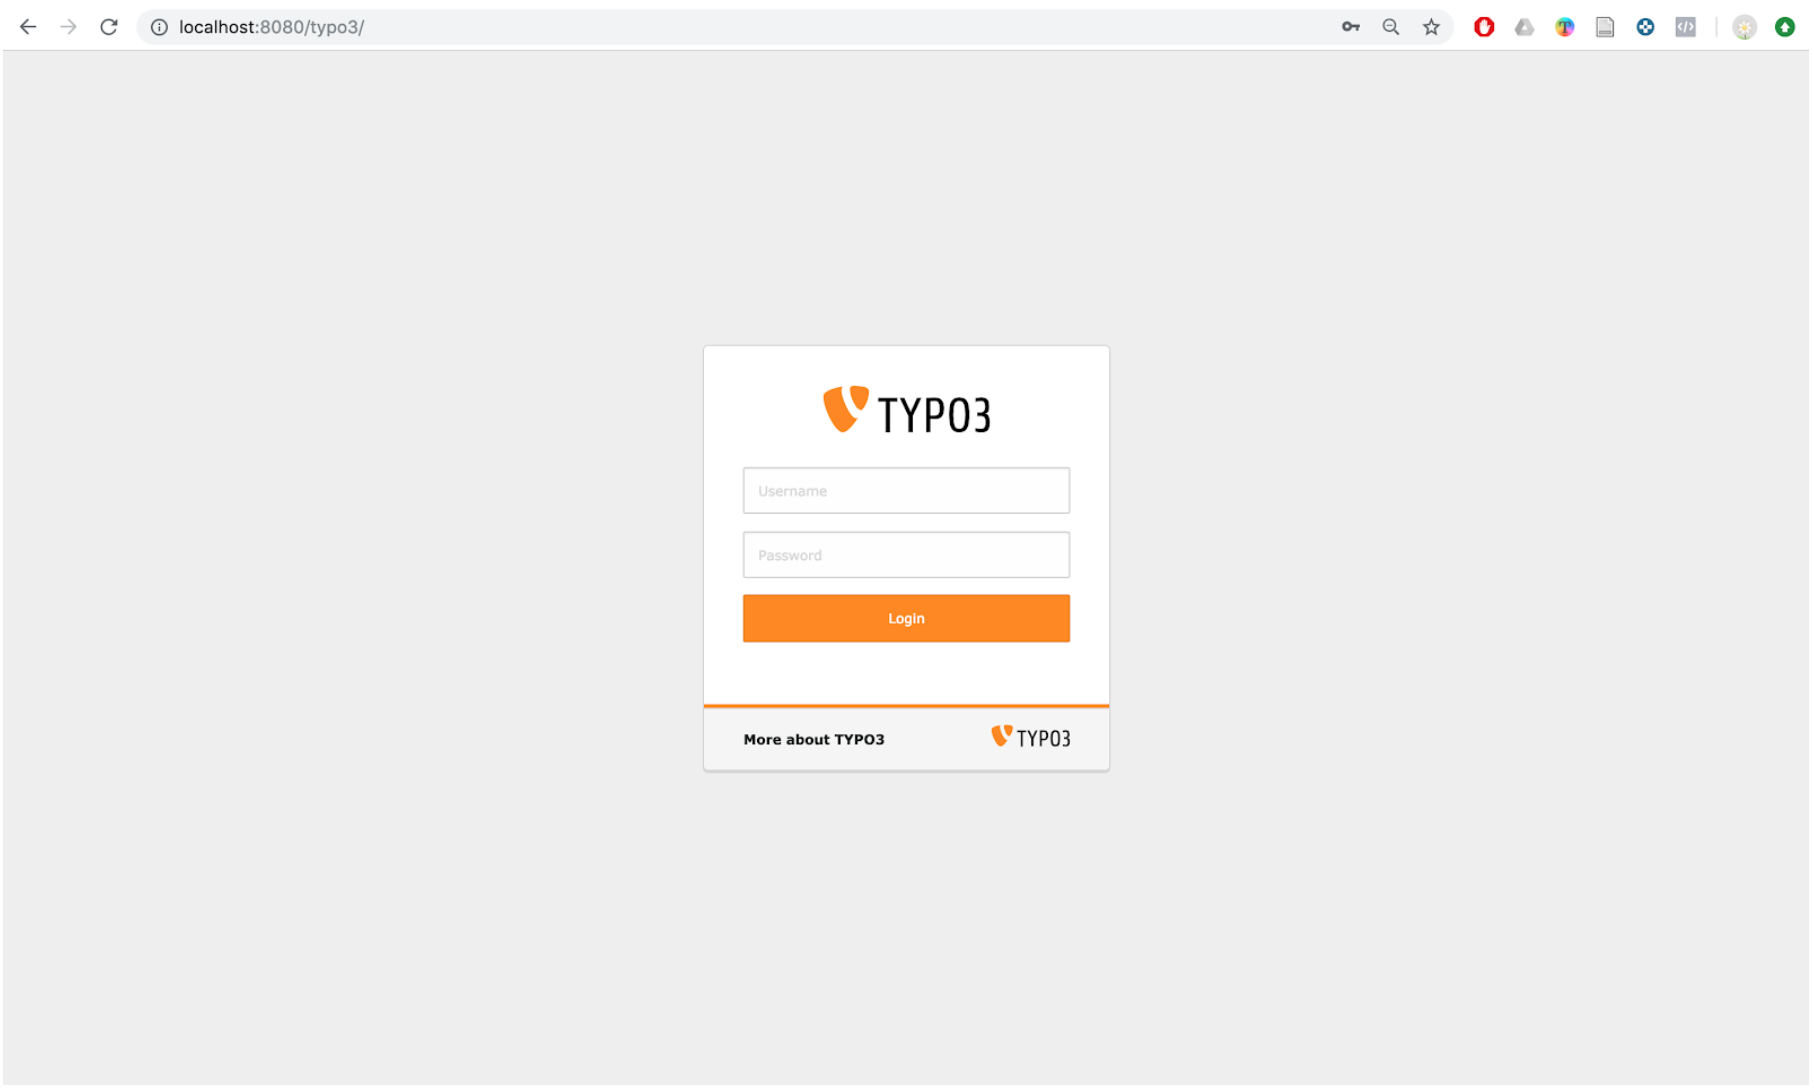
\includegraphics[width=12cm]{Figures/paula/typo3/typo_3_login.png}
\caption{Das Login-Fenster für TYPO3 im Browser}
\label{img:typo_3_login}
\end{figure}


\cleardoublepage

\section{TYPO3}
\subsection{Allgemein}

TYPO3 ist ein freies Content-Management-System für Webseiten, es wird in Frontend und Backend getrennt. Als Frontend wird die Präsentationsebene bezeichnet, das ist der Teil einer Applikation, den der Betrachter sehen kann. Als Backend hingegen, bezeichnet man die Datenzugriffsebene, das ist der Teil einer Applikation, welcher nicht für den Besucher sichtbar ist. Das Backend ist der Verwaltungsbereich einer Webseite. TYPO3 wird auf einem Webserver installiert und über den Webbrowser benutzt.

Das Backend beinhaltet die Programmierung einer Applikation und den Administrationsbereich. Im Gegensatz dazu das Frontend, das ist die tatsächliche Webseite, die der Endbenutzer im Browser sieht, also die Benutzeroberfläche.

\subsection{Login}

Damit niemand unbefugter im Frontend sowie Backend etwas verändern kann, muss man sich zuerst ins Backend einloggen. Dies geschieht über den Aufruf der Domain \textbf{localhost:80/typo3/} im Webbrowser (siehe Abbildung \ref{img:typo_3_login}).

\begin{figure}[ht!]
\centering
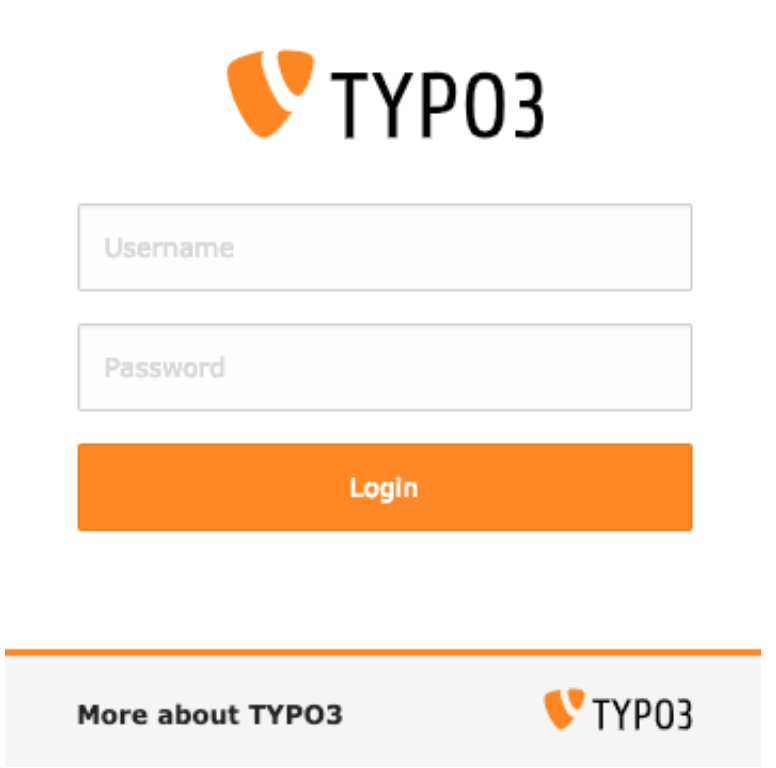
\includegraphics[width=8cm]{Figures/paula/typo3/login_TYPO3.png}
\caption{Das Login-Fenster für TYPO3}
\label{img:typo_3_logIn}
\end{figure}

Im Login-Fenster kann der Benutzername sowie das Passwort eingetragen werden (siehe Abbildung \ref{img:typo_3_logIn}). Beim ersten Login ist der \textbf{Benutzername: admin} und das \textbf{Passwort: visit-admin}, dieser muss in weiterer Folge geändert werden. Mehr dazu siehe Absatz zur Anpassung.
Nach einem erfolgreichen Login wird das Backend mit den dazugehörigen Modulen im Browser geladen.

\begin{figure}[ht!]
\centering
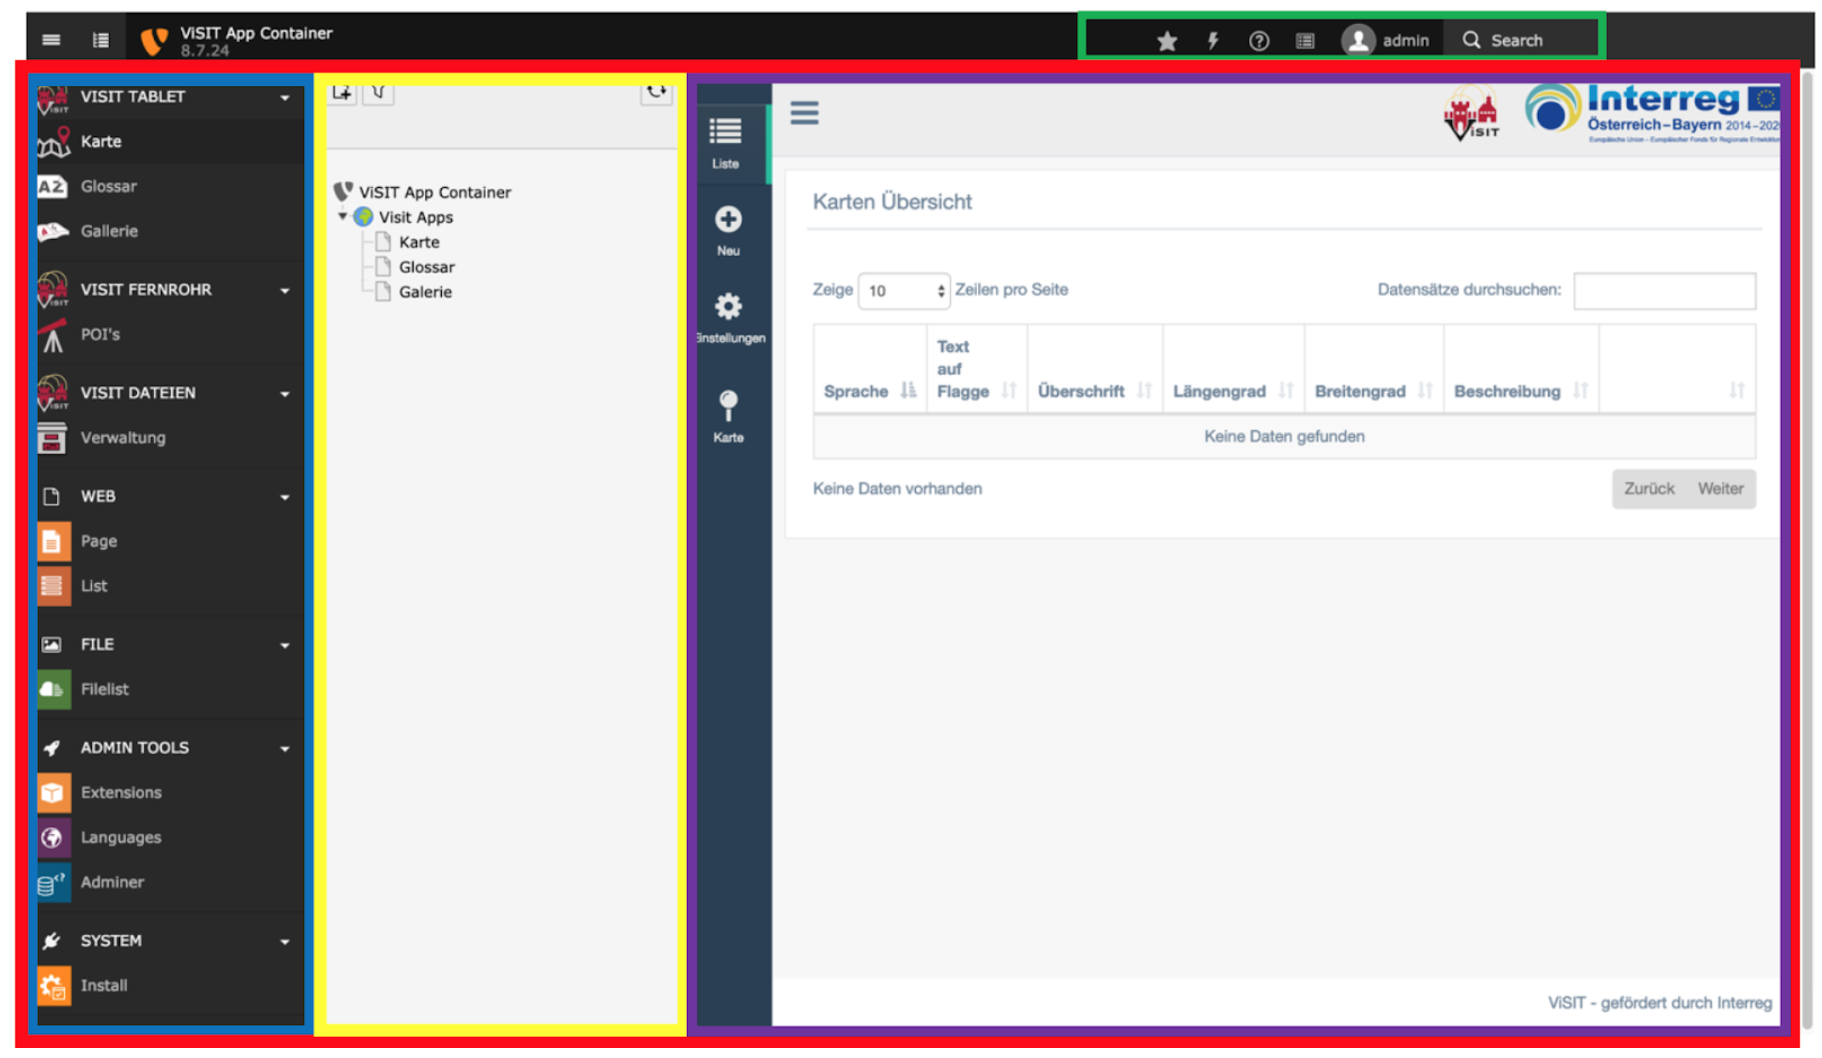
\includegraphics[width=12cm]{Figures/paula/typo3/aufbau_TYPO3.png}
\caption{Aufbau des TYPO3-Backends}
\label{img:typo_3_backend}
\end{figure}

\subsection{Aufbau von TYPO3}

Das TYPO3-Backend besteht aus einem Kopfbereich (grün eingerahmt) und einem Hauptbereich (rot eingerahmt), welcher aus drei Spalten besteht (siehe Abbildung \ref{img:typo_3_backend}). Im Kopfbereich kann der Administrator seine TYPO3-Benutzereinstellungen konfigurieren. Im Hauptbereich werden Webdokumente bearbeitet. Das TYPO3-Backend wird von links nach rechts abgearbeitet.

\subsubsection{Kopfleiste}

Die Kopfleiste bietet die Möglichkeit, die im TYPO3 Backend gespeicherten Lesezeichen aufzurufen (Stern-Symbol), den TYPO3 Cache der gesamten Webseite zu leeren (Blitz-Symbol) sowie Hilfe und Dokumentationen (Fragezeichen) zu TYPO3 aufzurufen. Das vierte Symbol zeigt die wichtigsten Systeminformationen an. Mit einem Klick auf den Benutzernamen, in der Grafik “admin”, öffnet sich ein Kontext-Menü mit der Möglichkeit Einstellungen an seinem Benutzer vorzunehmen oder sich aus dem TYPO3 Backend auszuloggen. Rechts neben dem Benutzer befindet sich das Suchfeld, mit dem sich das gesamte TYPO3 Backend durchsuchen lässt.

\subsubsection{Die Spalten des Hauptbereichs}

\textbf{Linke Spalte:} \textit{Modulleiste} (blau eingerahmt), hier kann das Modul ausgewählt werden, welches bearbeitet werden soll (siehe Abbildung \ref{img:typo_3_backend}).\\

\textbf{Mittlere Spalte:} \textit{Seitenbaum} (gelb eingerahmt), hier wird die zu bearbeitende TYPO3-Seite ausgewählt. Der Seitenbaum ist das zentrale Element, wenn es darum geht sich durch die Webseite zu navigieren. Hier wird der Aufbau und die Seitenhierarchie der Webseite in einer Struktur abgebildet, die der Ordnerstruktur ähnlich ist. Einzelne Seiten können Unterseiten enthalten, die im Seitenbaum eingerückt dargestellt werden (siehe Abbildung \ref{img:typo_3_backend}).\\

\textbf{Rechte Spalte:} \textit{Arbeitsbereich} (violett eingerahmt), hier wird am ausgewählten TYPO3-Objekt gearbeitet (siehe Abbildung \ref{img:typo_3_backend}).

\subsection{Konfiguration des Backends mit TYPO3}

Die für die Applikationen benötigten TYPO3 Extensions werden automatisch installiert, sollte eine weitere Extension benötigt werden, befindet sich eine Anleitung für die Installation in diesem Abschnitt. Extensions sind optionale Software-Komponenten, also Zusatzmodule, die eine bestehende Software erweitern.\\

Installation von TYPO3 Extensions: Dazu wird in der linken Spalte zuerst das Modul “Extensions” ausgewählt. Dann erscheinen im Hauptfenster verschiedene Extensions, welche alphabetisch gelistet sind. Bei der Erstinstallation werden folgende Extensions (unten ist der Key angegeben, welcher sich in der mittleren Spalte befindet) automatisch installiert (siehe Abbildung \ref{img:typo3_extensions}):

\begin{itemize}
    \item visit\_tablets
    \item scheduler
    \item tstemplate
    \item fluid\_styled\_content
    \item setup
\end{itemize}

\begin{figure}[ht!]
\centering
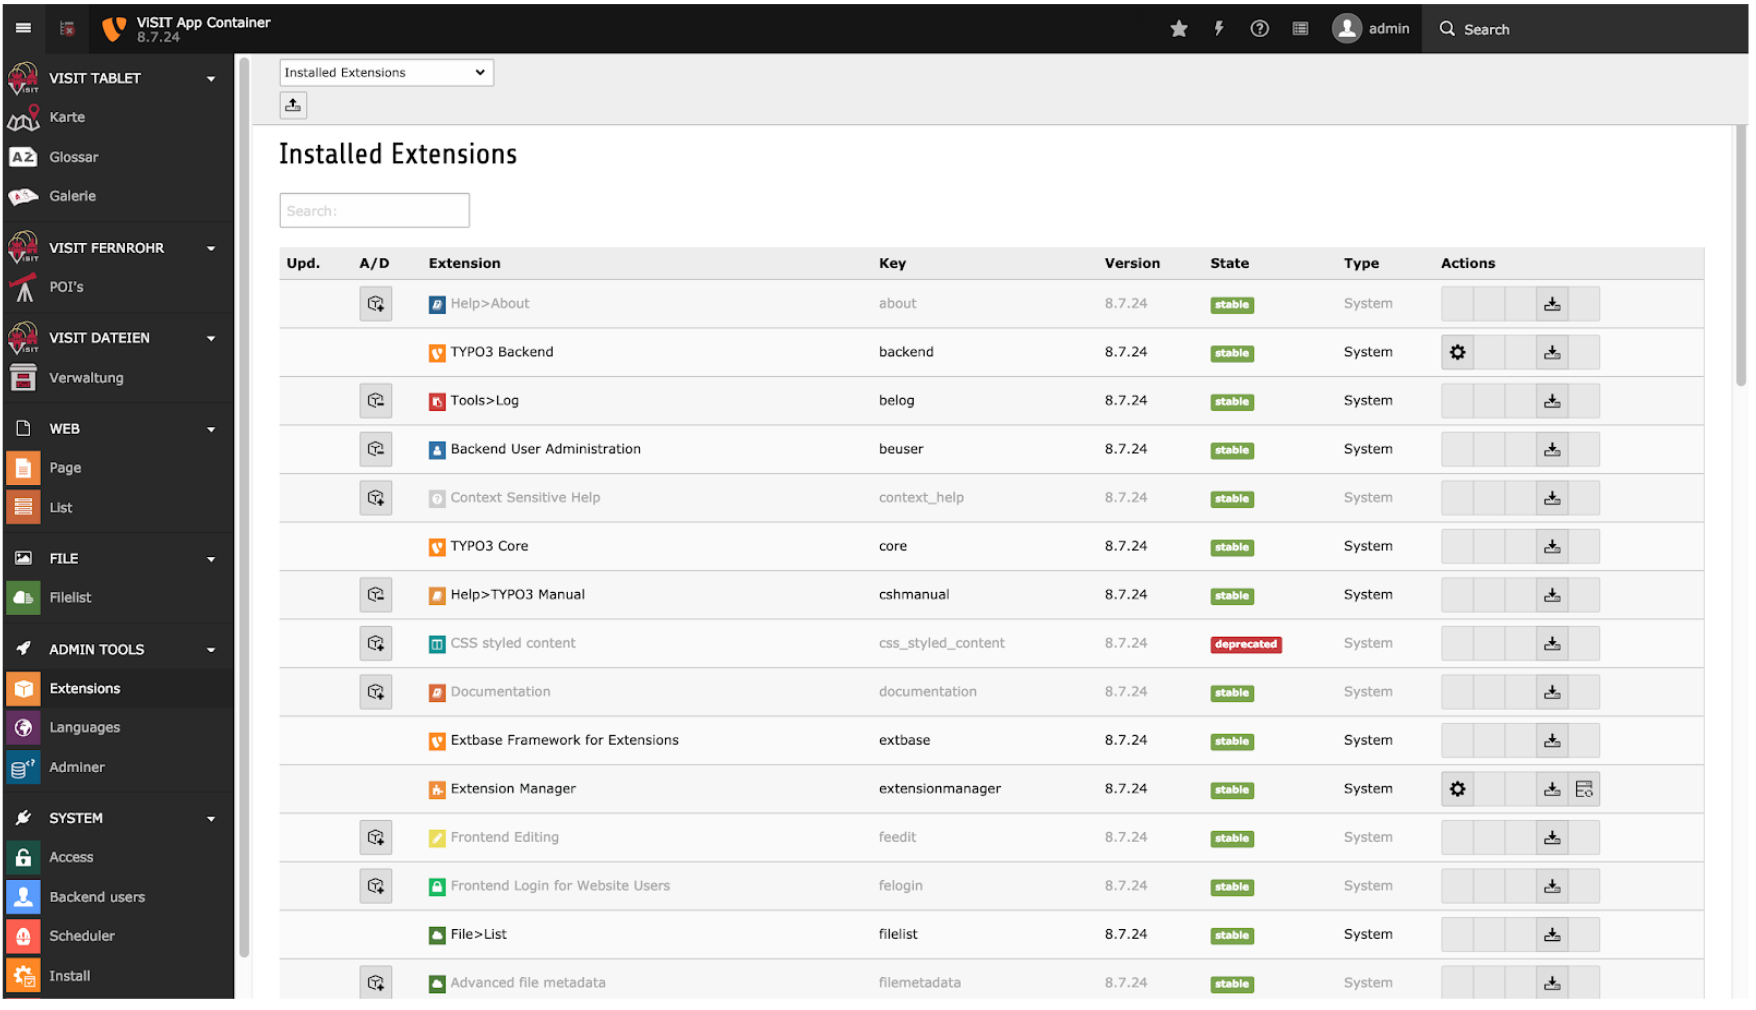
\includegraphics[width=12cm]{Figures/paula/typo3/typo3_extensions.png}
\caption{Installation der Extensions}
\label{img:typo3_extensions}
\end{figure}

Mittels einem Klick auf das Würfelsymbol mit einem Plus werden die oben angegebenen Extensions der Reihe nach aktiviert (siehe Abbildung \ref{img:typo3_extensions}). Die aktivierten Extensions erscheinen dann als auswählbare Module in der linken Spalte.
Optional kann im nächsten Schritt die Sprache Deutsch installiert werden, sonst ist die Hauptsprache Englisch. Um die Sprache zu installieren, wird in der linken Spalte unter den ADMIN TOOLS \glqq Languages\grqq{} ausgewählt (siehe Abbildung \ref{img:sprache_aendern}).

\begin{figure}[ht!]
\centering
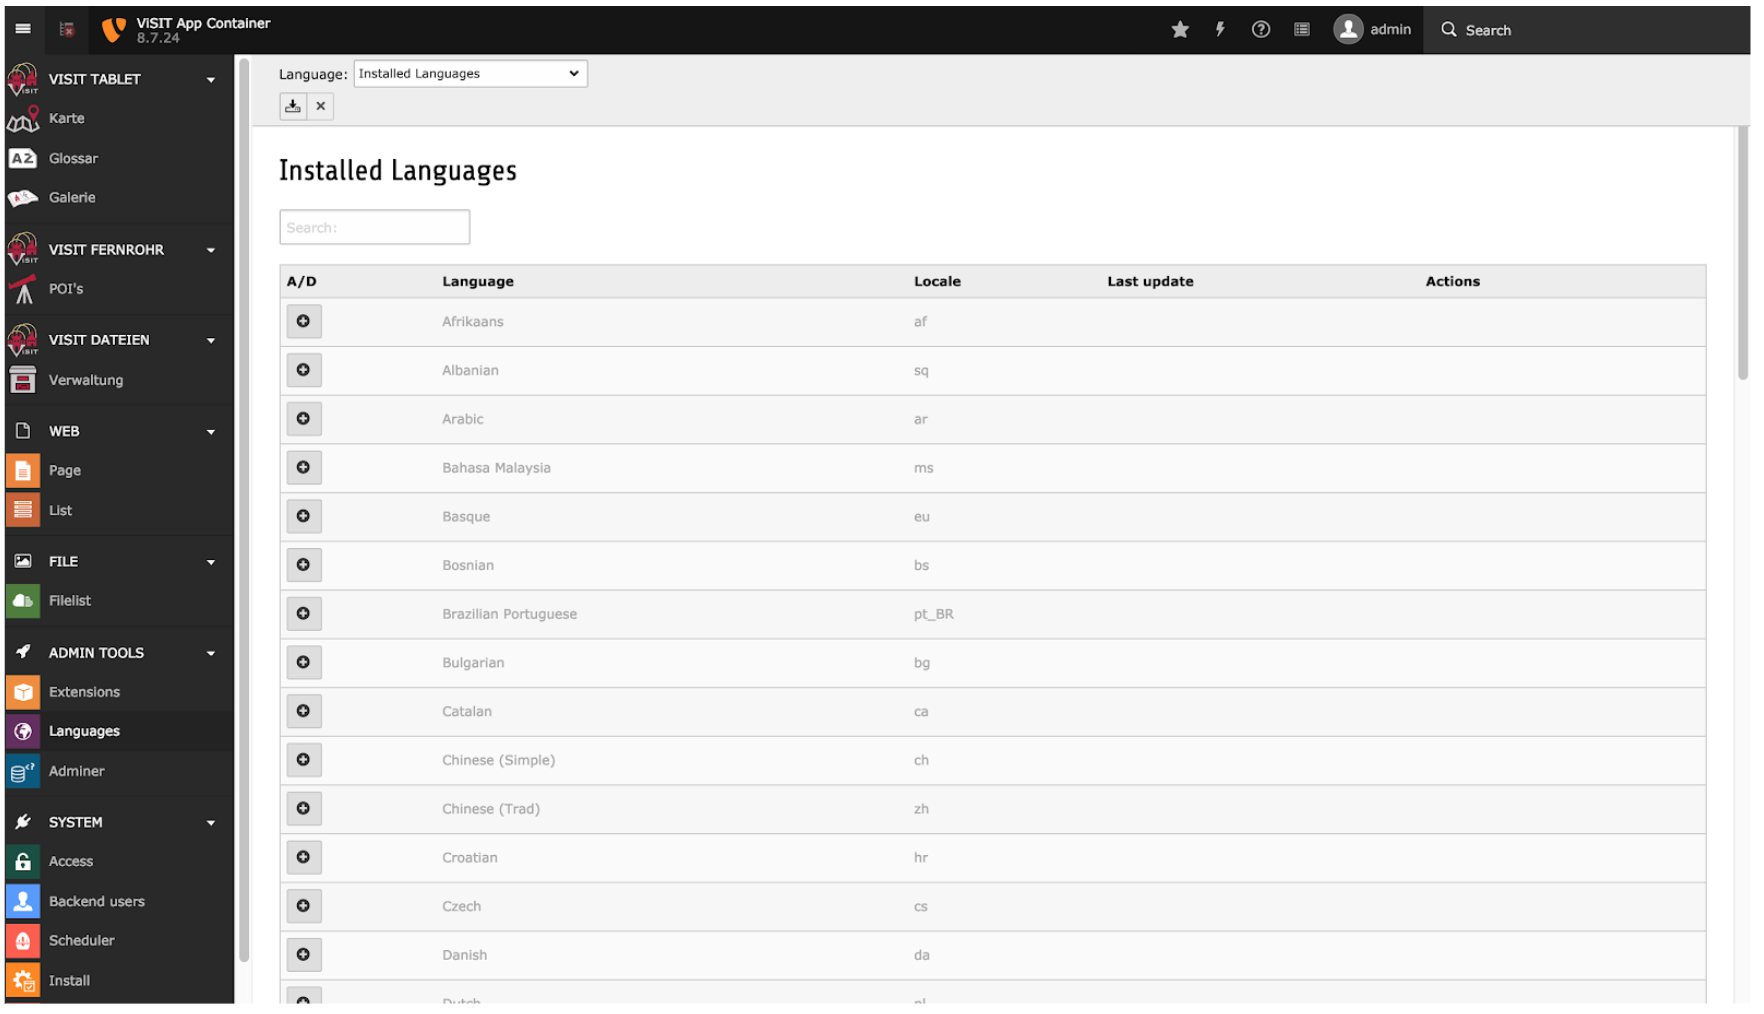
\includegraphics[width=12cm]{Figures/paula/typo3/sprache_aendern.png}
\caption{Änderung der Sprache}
\label{img:sprache_aendern}
\end{figure}

Im Hauptfenster erscheinen nach dem Klick die unterstützten Sprachen, hier \glqq German\grqq{} suchen und zuerst mittels einem Klick auf das Plus-Symbol links von der Sprache die Sprache aktivieren, dabei erscheint oben rechts eine grüne Meldung mit \glqq Success, language was successfully activated.\grqq{}. Als nächstes muss die aktivierte Sprache mittels Klick auf das Download-Symbol rechts von der Sprache heruntergeladen werden. War der Download erfolgreich, so erscheint oben rechts eine grüne Meldung mit \glqq Success. The translation update has been successfully completed.\grqq{}.

\subsection{Anpassung}

Im Kopfbereich können die TYPO3-Benutzereinstellungen konfiguriert werden. Dazu wird im Kopfbereich oben rechts zuerst der Benutzer ausgewählt. Bei der Erstinstallation ist es der \glqq admin\grqq{}, dabei wird ein Menü aufgeklappt, aus welchem die \glqq User settings\grqq{} ausgewählt werden (siehe Abbildung \ref{img:benutzereinstellungen}).

\begin{figure}[ht!]
\centering
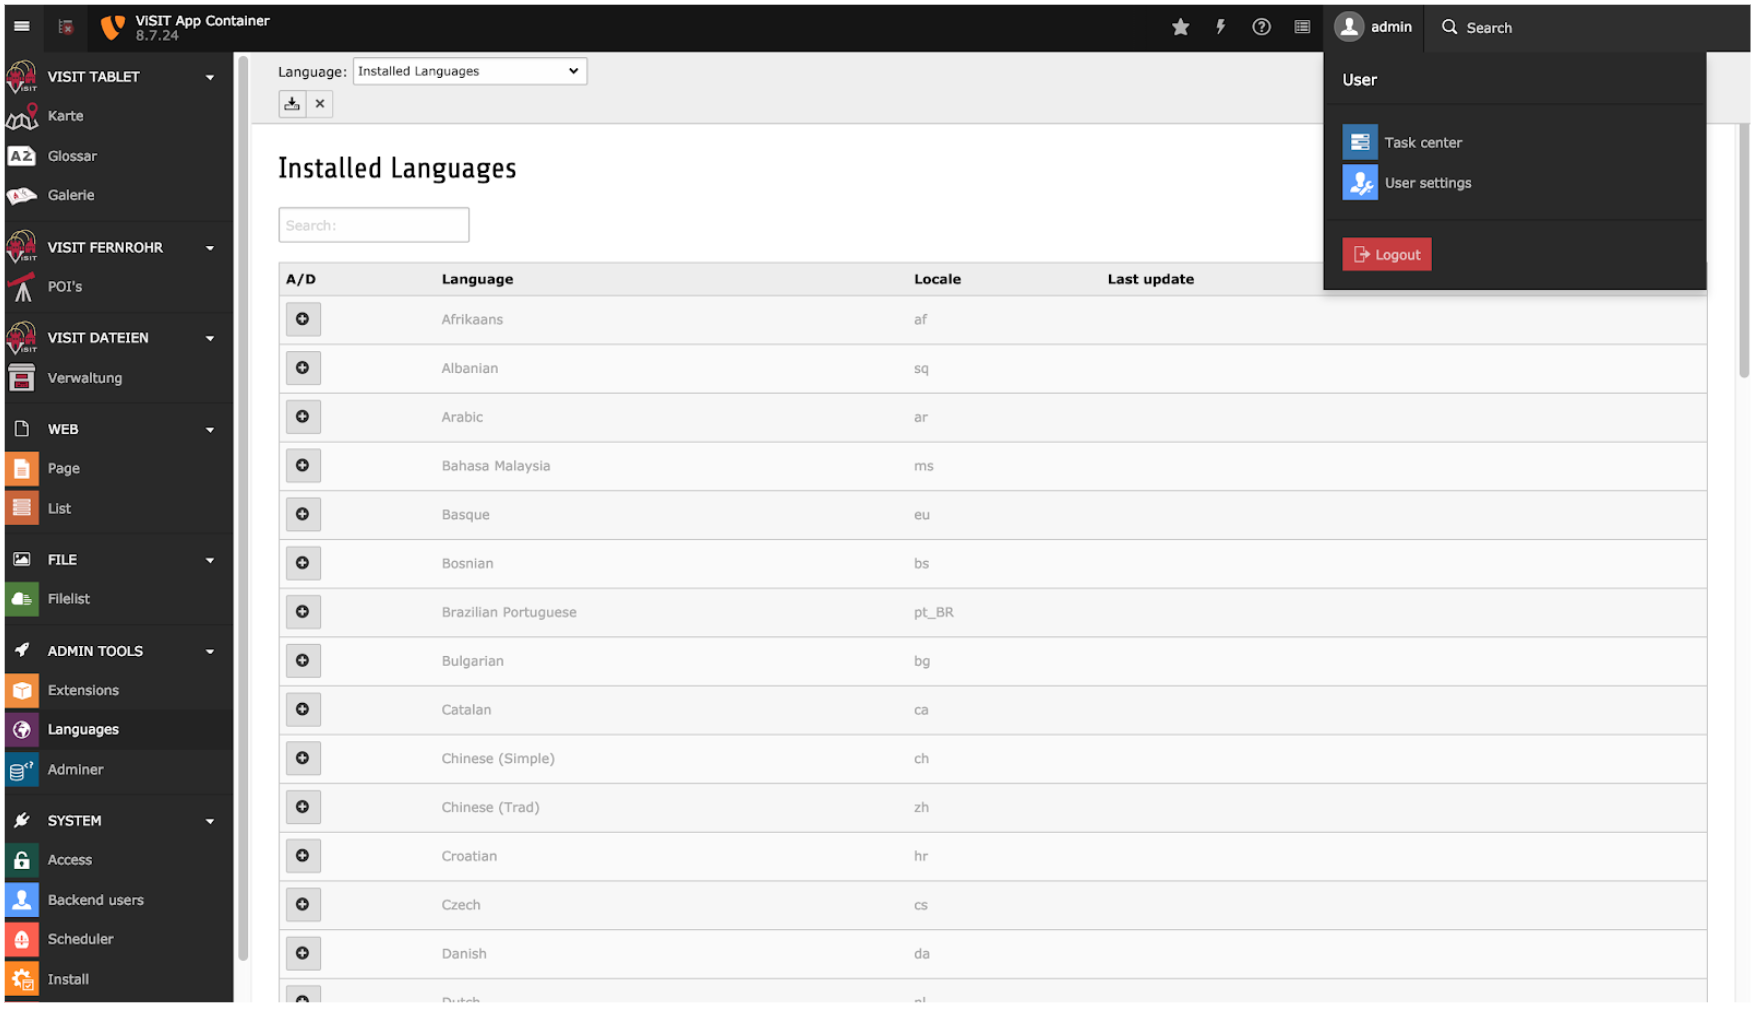
\includegraphics[width=12cm]{Figures/paula/typo3/benutzereinstellungen.png}
\caption{Konfiguration der Benutzereinstellungen}
\label{img:benutzereinstellungen}
\end{figure}

Jetzt erscheinen im Hauptbereich die User Settings, welche in dieser Maske konfiguriert werden können. Jetzt kann zuerst die Sprache umgestellt werden. Dies kann gleich im ersten Raster \glqq Personal data\grqq{}, im unteren Bereich unter Languages geändert werden (siehe Abbildung \ref{img:benutzereinstellungen_sprache}). Hier kann die heruntergeladene Sprache mittels Dropdown ausgewählt werden. Damit die Auswahl auch gespeichert und angewendet wird, muss auf das Speicher-Symbol (Diskette) ganz oben links im Hauptfenster geklickt werden. Nur durch diesen Klick werden die User Settings upgedated und die Sprache auch angewendet. Jetzt erscheinen oben im Hauptfenster drei Meldungen. Die grüne Meldung besagt, dass die Settings upgedated wurden. Die blaue Meldung sagt, dass die Seite (localhost:80/typo3/) neu geladen werden muss, um die Veränderungen zu aktivieren. Die rote Meldung sagt, dass das neue Passwort nicht upgedated wurde, da es nicht zweimal eingegeben wurde.\\

\begin{figure}[ht!]
\centering
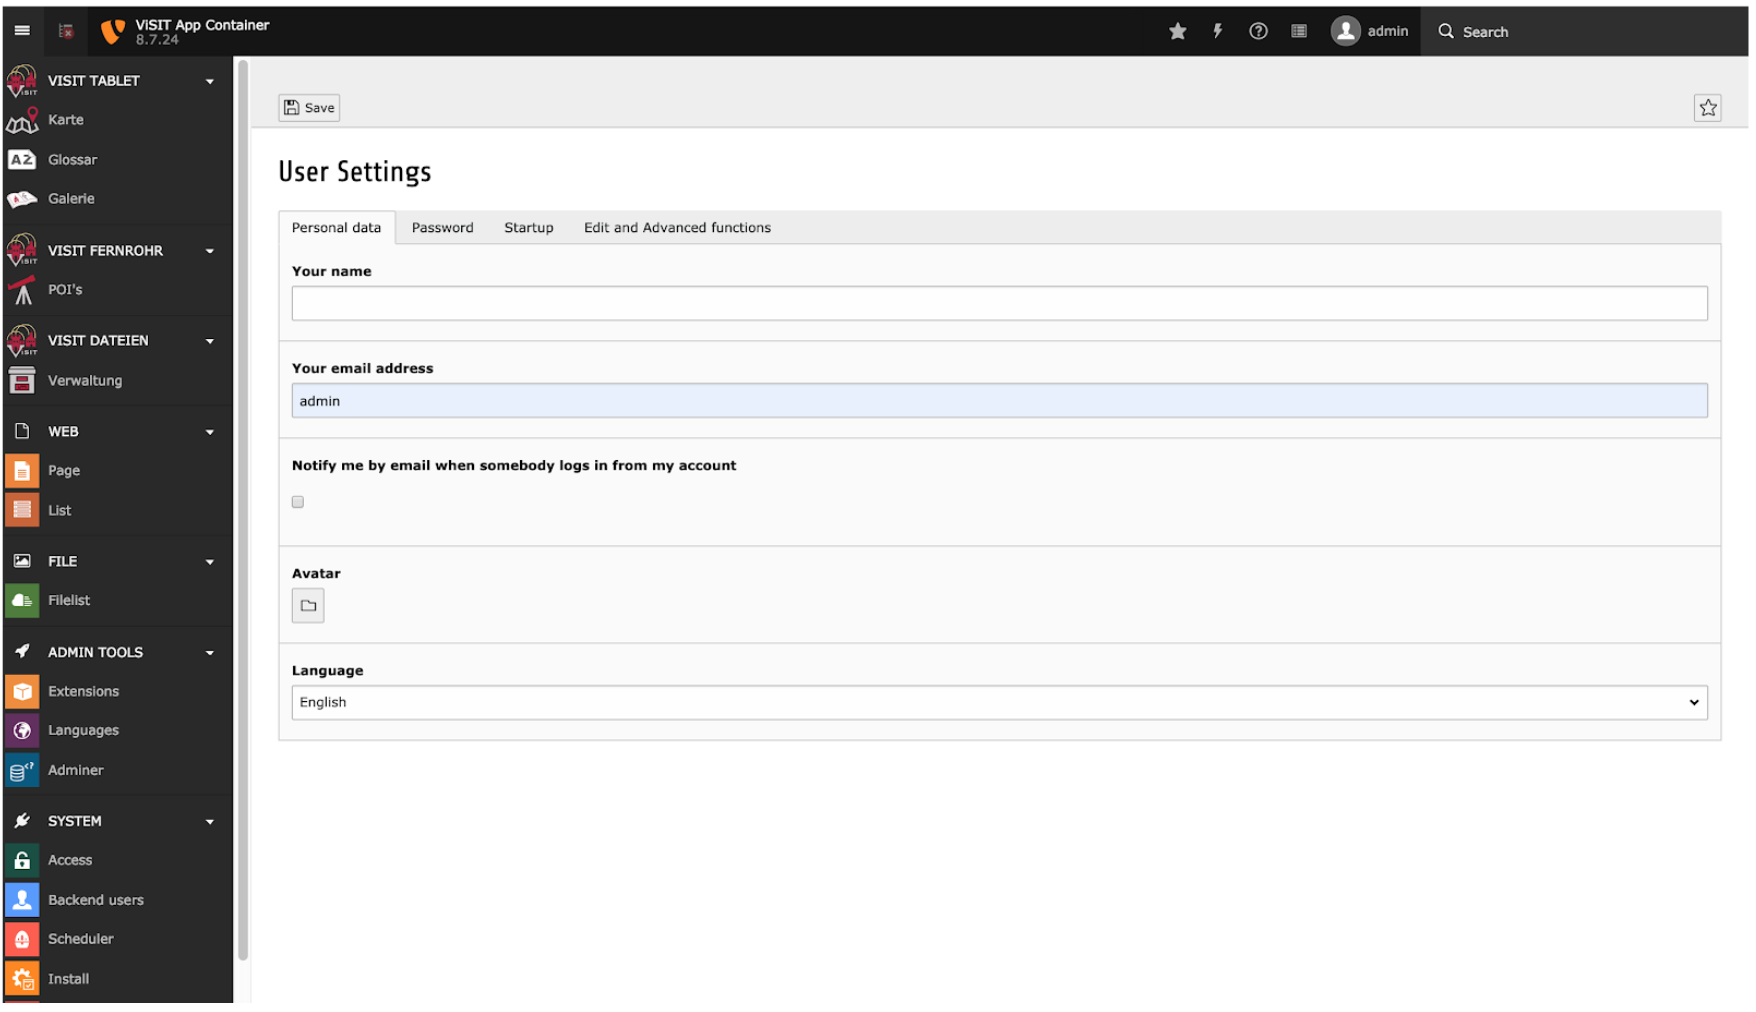
\includegraphics[width=12cm]{Figures/paula/typo3/benutzereinstellungen_sprache.png}
\caption{Änderung der Benutzereinstellungen und der Sprache}
\label{img:benutzereinstellungen_sprache}
\end{figure}

Als nächstes wird das Passwort geändert. Dazu wird die Registerkarte \glqq Password\grqq{} ausgewählt (siehe Abbildung \ref{img:aenderung_passwort}). Jetzt erscheint das zuvor eingegebene Passwort \glqq visit-admin\grqq{} als eine Punkte-Kette in der ersten Zeile, hier kann das Passwort mit einem neuen Passwort überschrieben werden. Gleiches Passwort wird in der darunter liegenden Zeile nochmals eingegeben. Damit die Änderungen gespeichert werden, wird wieder oben links das Speichern-Symbol geklickt. Ab jetzt werden auch die Änderungen der Sprache angewendet und alles wird auf Deutsch angezeigt. Mit diesem Schritt ist das Backend fertig vorbereitet.

\begin{figure}[ht!]
\centering
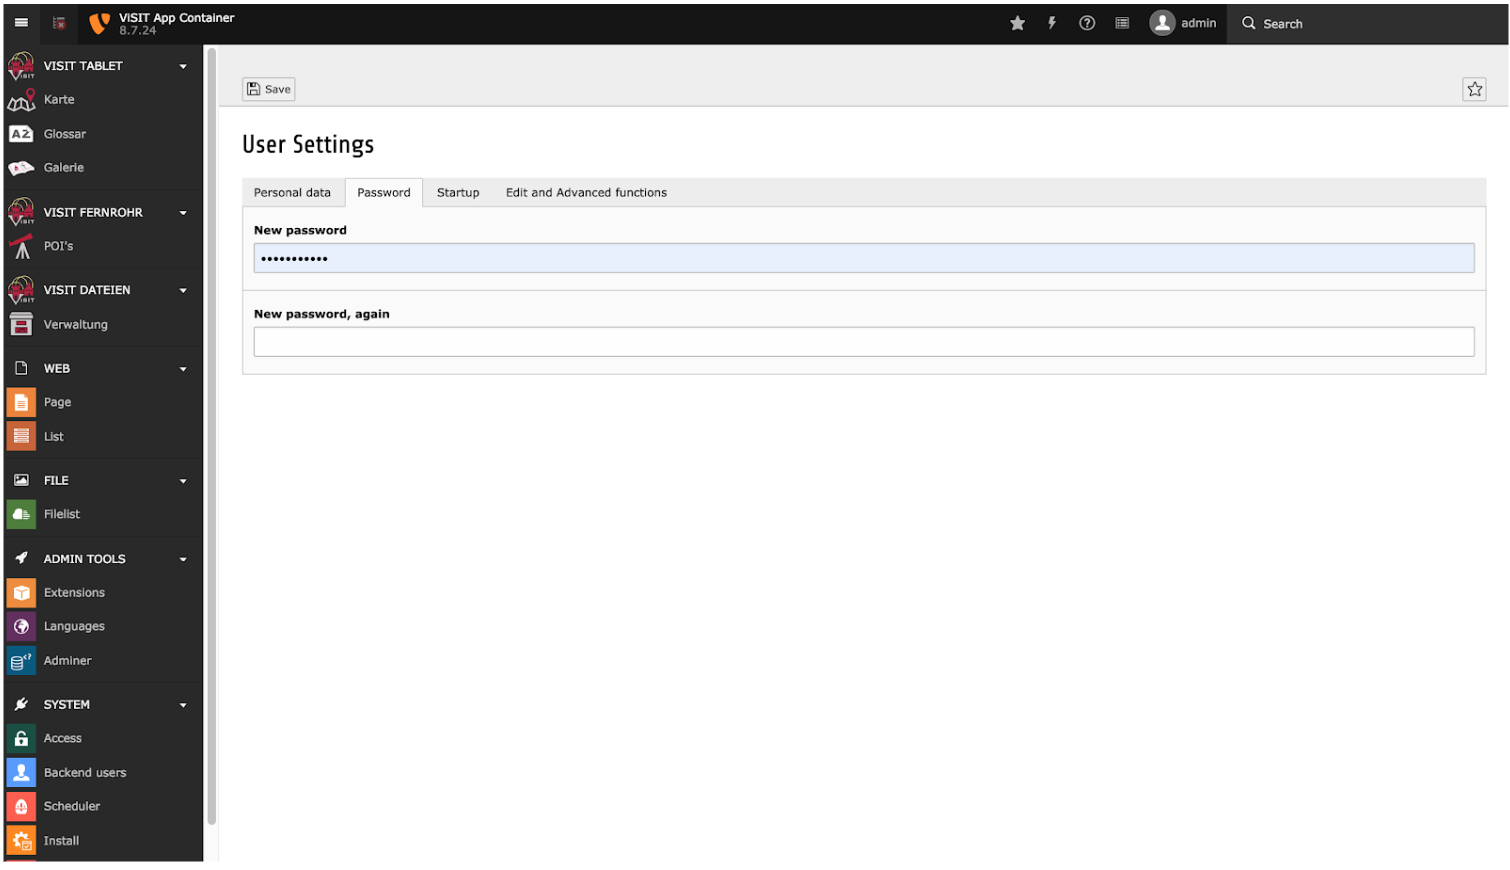
\includegraphics[width=12cm]{Figures/paula/typo3/aenderung_passwort.png}
\caption{Änderung des Passworts}
\label{img:aenderung_passwort}
\end{figure}

\subsection{Hinzufügen einer Applikation aus dem App-Bundle}

Dazu wird in der linken Spalte \glqq Seite\grqq{} ausgewählt. Jetzt kann dem ViSIT App Container eine Seite hinzugefügt werden. Zuerst muss auf das oben ganz links befindlichen Seiten-Symbol geklickt werden, dann erscheint eine Auswahl an möglichen Aktionen. Hier das erste leere Seite-Symbol anklicken und auf den darunter befindlichen ViSIT App Container ziehen und darüber loslassen, anschließend kann der Seite ein Name gegeben werden (siehe Abbildung \ref{img:neue_seite_hinzufuegen}).

\begin{figure}[ht!]
\centering
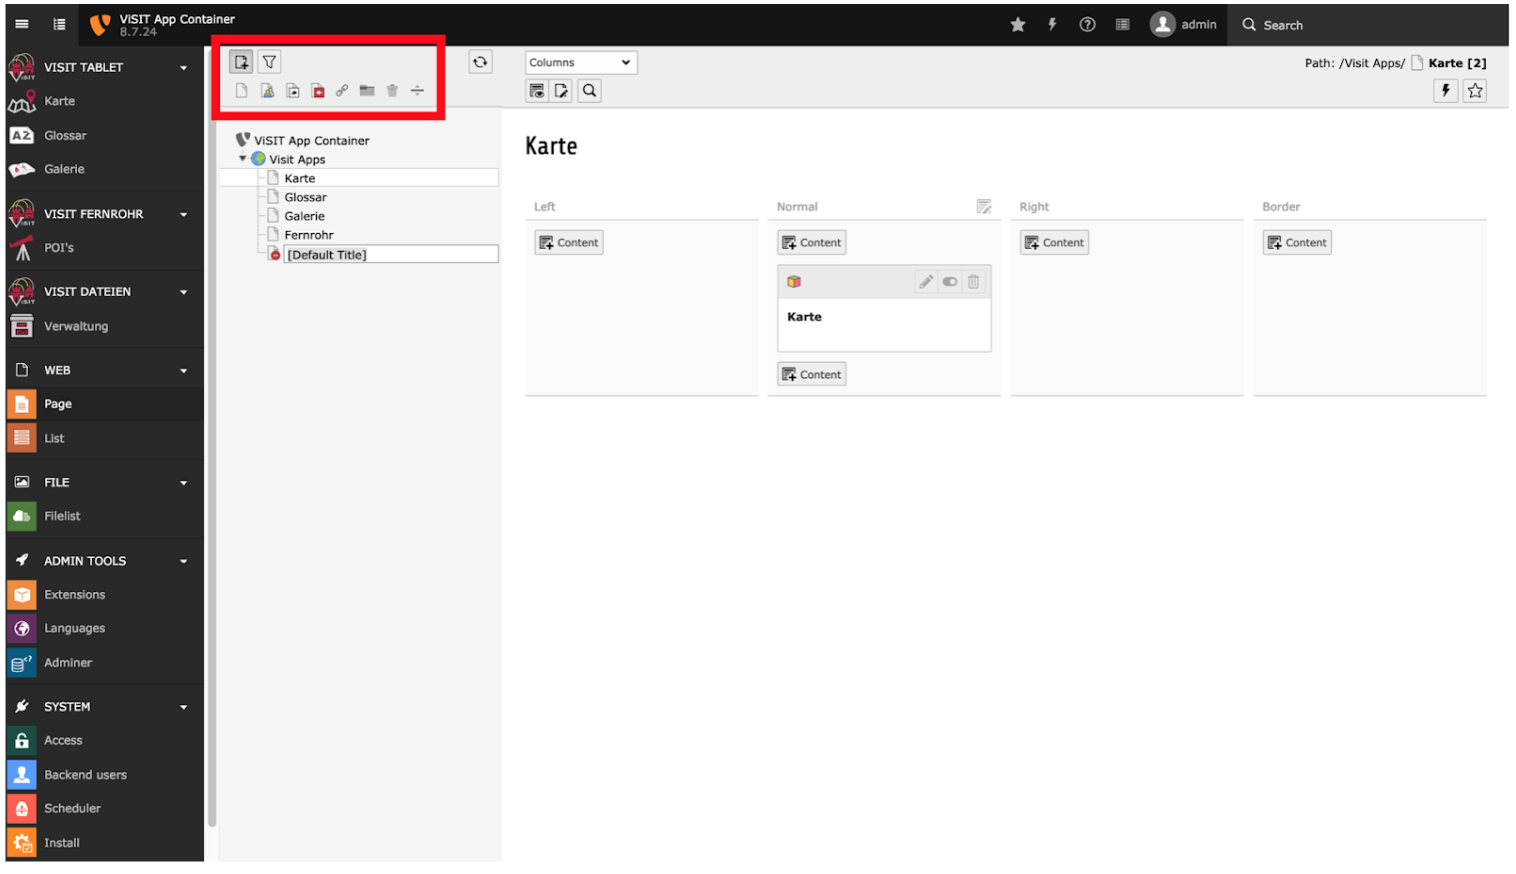
\includegraphics[width=12cm]{Figures/paula/typo3/neue_seite_hinzufuegen.png}
\caption{Hinzufügen einer neuen Seite}
\label{img:neue_seite_hinzufuegen}
\end{figure}

Mittels Rechtsklick auf die soeben erstellte Seite erscheint unter der Seite ein weiteres Menü, aus diesem dann \glqq Bearbeiten\grqq{} auswählen. Danach kann rechts die Seite konfiguriert werden.\\

Im nächsten Schritt muss das Verhalten der Seite konfiguriert werden. Dazu den Raster \glqq Verhalten\grqq{} anklicken und unter \glqq Sonstige\grqq{} \glqq Als Anfang der Website benutzen\grqq{} aktivieren.
Dann den Raster \glqq Zugriff\grqq{} auswählen und unter \glqq Sichtbarkeit\grqq{} \glqq Seite\grqq{} deaktivieren.
Nachdem die Änderungen durchgeführt wurden, müssen diese gespeichert werden. Dazu muss auf das Speicher-Symbol oben auf der Hauptseite geklickt werden. Danach erscheint ein Weltkugel-Symbol neben der soeben erzeugten Seite im linken Teil des Hauptfensters.

\subsection{Erzeugung des Layouts}

Um das Layout der Seite zu definieren, muss auf die soeben erzeugte Seite geklickt werden (siehe Abbildung \ref{img:layout_erzeugung}).

\begin{figure}[ht!]
\centering
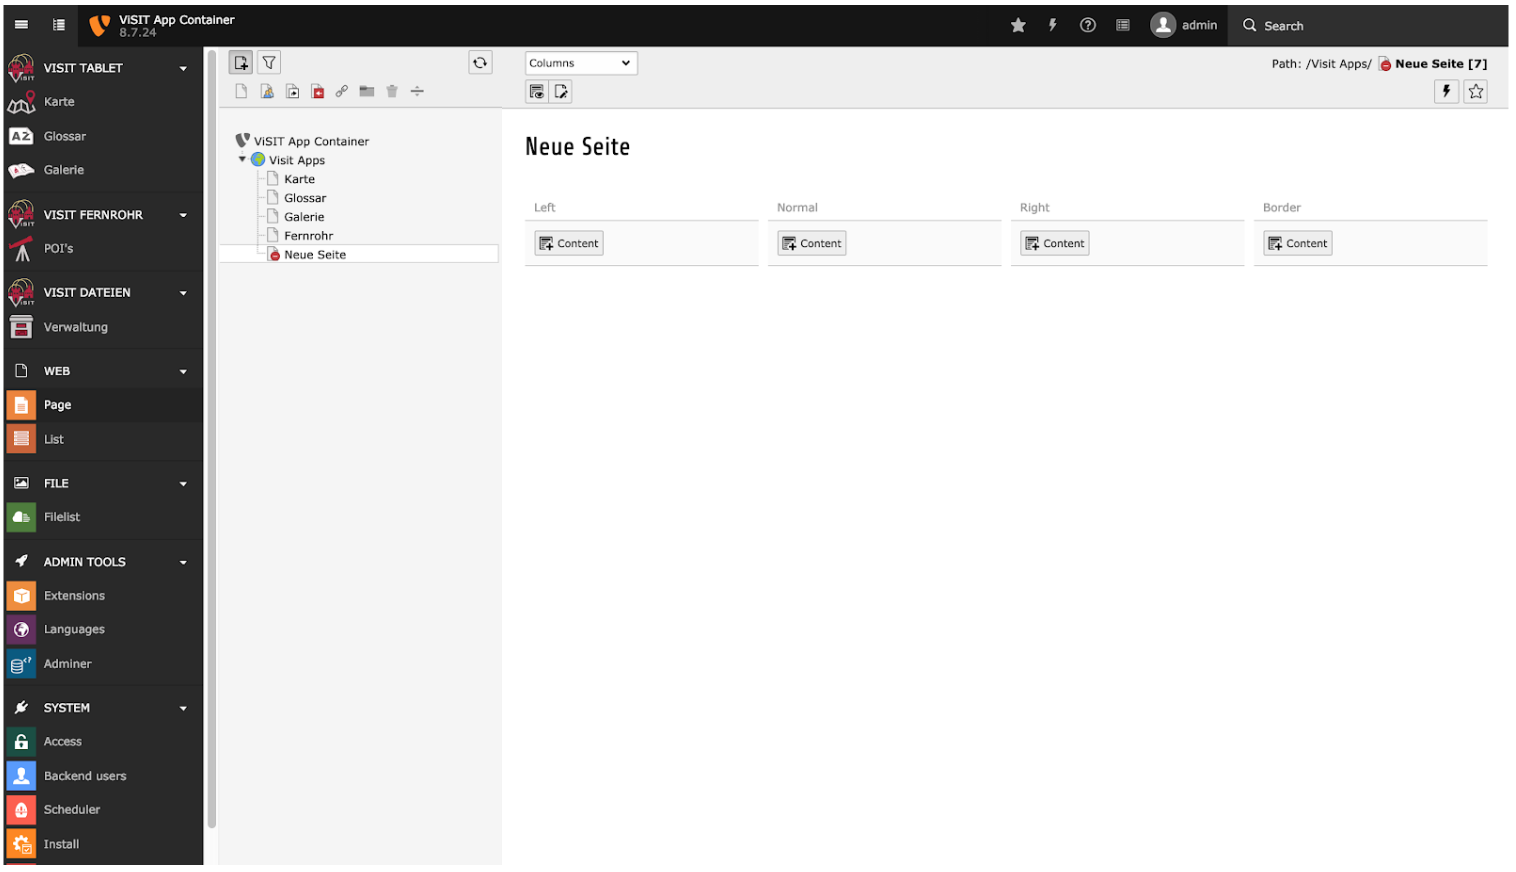
\includegraphics[width=12cm]{Figures/paula/typo3/layout_erzeugung.png}
\caption{Erzeugung des Layouts der neu erstellten Seite}
\label{img:layout_erzeugung}
\end{figure}

Im rechten Teil des Hauptfensters erscheinen vier Möglichkeiten der Inhaltspositionierung. Für die ViSIT-Applikationen wird die normale Inhaltspositionierung benötigt.  Um weitere Konfiguration durchzuführen, unter \glqq Normal\grqq{} auf das das Inhalts-Symbol klicken und im Raster \glqq Plug-Ins\grqq{} auswählen, hier können die Plugins für die jeweilige ViSIT-Applikation ausgewählt werden (siehe Abbildung \ref{img:auswahl_plugins}).

\begin{figure}[ht!]
\centering
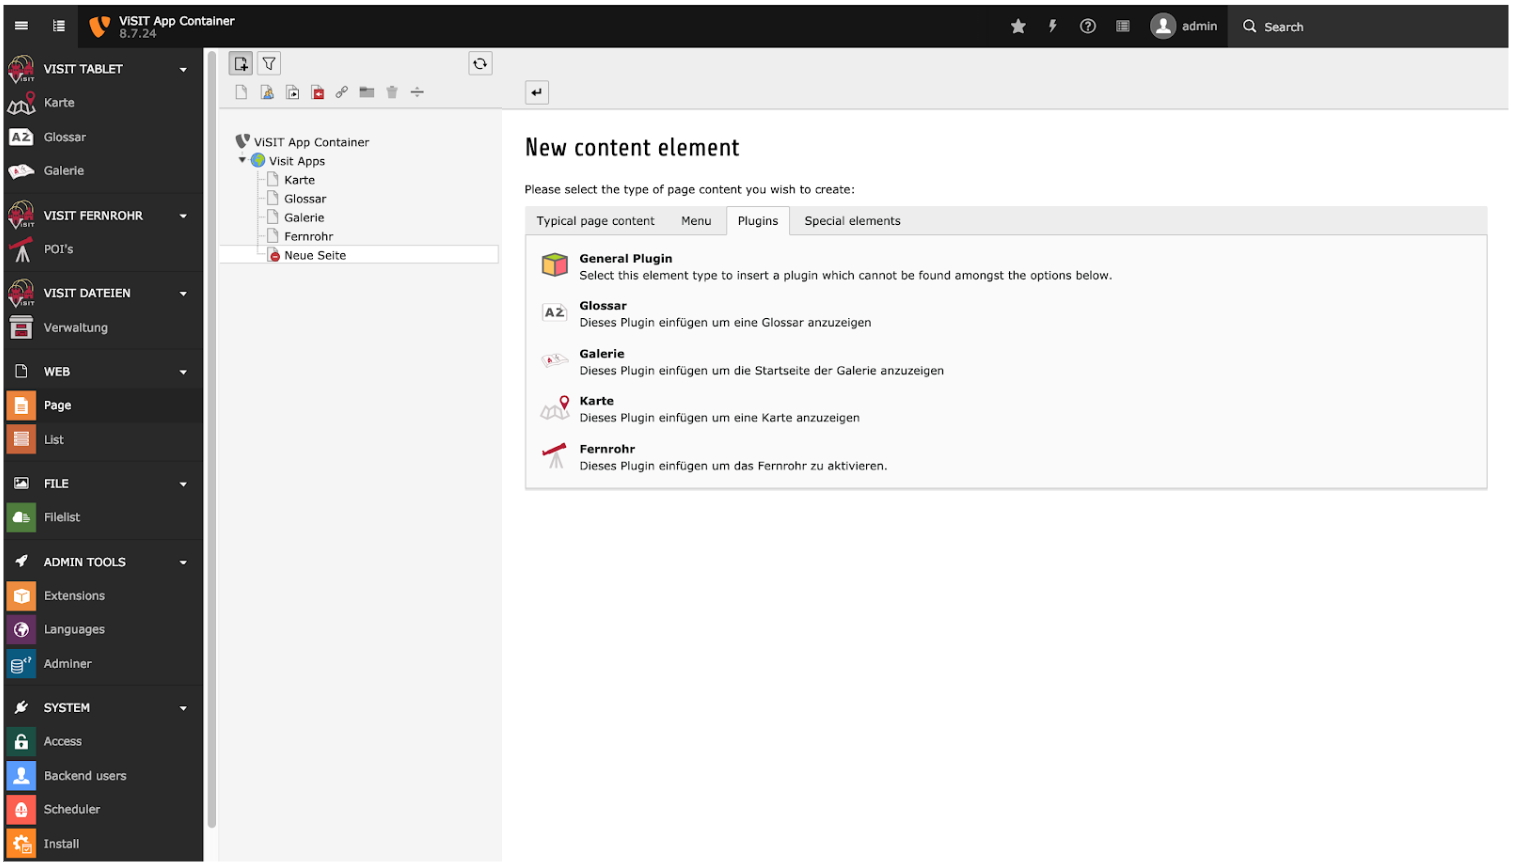
\includegraphics[width=12cm]{Figures/paula/typo3/auswahl_plugins.png}
\caption{Auswahl der Plug-Ins}
\label{img:auswahl_plugins}
\end{figure}

\subsection{Das Karten-Plug-In}

Im Raster \glqq Plug-Ins\grqq{} die \glqq Karte - Dieses Plugin einfügen um eine Karte anzuzeigen\grqq{} auswählen und oben auf das Speicher-Symbol klicken, damit die Änderungen gespeichert werden. Nach dem Speichern kann die Seite mit dem X-Symbol über der Überschrift geschlossen werden. Danach erscheint die Übersicht über die erzeugte Seite, hier sieht man, dass das Karten-Plugin eingebunden wurde (siehe Abbildung \ref{img:einbindung_plugins}).

\begin{figure}[ht!]
\centering
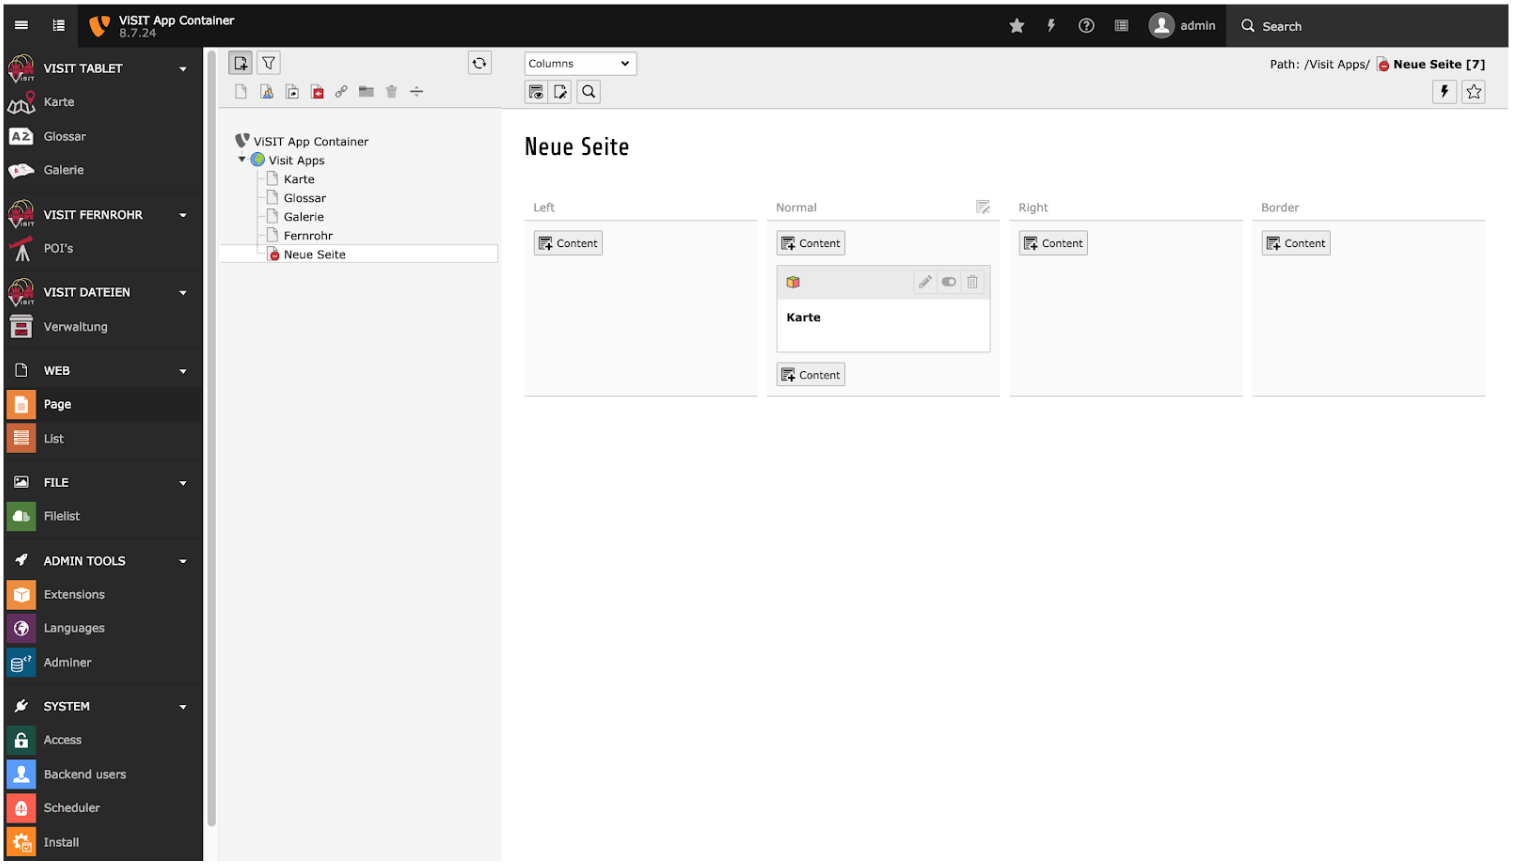
\includegraphics[width=12cm]{Figures/paula/typo3/einbindung_plugin.png}
\caption{Einbindung eines Plug-Ins}
\label{img:einbindung_plugins}
\end{figure}

Wenn jetzt die soeben erstellte Seite in der linken Spalte des Hauptfensters, also da wo die Weltkugel ist, mit Rechtsklick ausgewählt, kommt ein Dropdown-Menü. Jetzt den ersten Eintrag \glqq Ansehen\grqq{} aus der Liste auswählen und die Seite kann im Browser angesehen werden.

\subsection{Erstellung eines Templates}

Wenn ein neuer Raum hinzugefügt wird, wird ein neuer Webroot benötigt, dieser wird mittels Template erzeugt und stellt den Seitenanfang der Webseite dar. Sollen mehrere gleiche Applikationen laufen, dann wird für jede einzelne Applikation ein eigenes Template benötigt.
Für die Darstellung der Inhalte auf der Webseite werden Templates verwendet. Ein Template ist eine Design- und Formatierungsvorlage für ein Dokument, es ist das Grundgerüst, welches mit Inhalten befüllt werden muss.\\

Um ein Template in TYPO3 zu erstellen, muss im ersten Schritt unter WEB das \glqq Template\grqq{} aus der Modul-Liste auf der linken Seite ausgewählt werden. Danach erscheinen die Template-Werkzeuge in der rechten Hälfte des Hauptfensters, hier kann \glqq Template für neue Website erstellen\grqq{} ausgewählt werden. Jetzt kann in der Werkzeugleiste des Hauptbereichs das Dropdown-Feld aufgemacht und \glqq Info/Bearbeiten\grqq{} ausgewählt werden. In der Übersicht im Hauptbereich erscheinen die wichtigsten Template-Informationen. Danach \glqq Vollständigen Template-Datensatz bearbeiten\grqq{} auswählen. Hier kann im Raster \glqq Allgemeines\grqq{} der Titel des Templates hinzugefügt werden, des weiteren muss der Inhalt aus \glqq Setup\grqq{} gelöscht werden.\\

Danach ins Raster \glqq Enthält\grqq{} wechseln, hier können verschiedene Objekte aus der rechten Spalte \glqq Verfügbare Objekte\grqq{} in die linke Spalte \glqq Ausgewählte Objekte\grqq{} verschoben werden, hier muss jedoch auf die Reihenfolge dieser Objekte geachtet werden. Hier zuerst auf \glqq Fluid Content Elements (fluid\_styled\_content)\grqq{} klicken, dann wandert dieses Objekt in die linke Spalte. Das gleiche mit dem Objekt \glqq tablets (visit\_tablets)\grqq{}. Jetzt befinden sich beide Objekte in der linken Spalte unter \glqq Ausgewählte Objekte\grqq{}. Damit diese Änderungen gespeichert werden, muss wieder auf das Speichern-Symbol über der Überschrift im Hauptbereicht geklickt werden. Wenn die Webseite auf dem localhost:80/ aufgerufen wird, erscheint die Karte.



\cleardoublepage

\section{Karten-Applikation}

In der Karten-Applikation sehen die Besucher auf dem Tablet eine Landkarte angezeigt. Auf dieser Landkarte befinden sich kleine Flaggen als Points of Interest (POI). Der Besucher kann auf eine Flagge tippen und dann öffnet sich rechts von der Karte ein seitlicher Infobereich mit näheren Informationen zur ausgewählten Flagge.

\subsection{Einpflegen der Daten in die Karten-Applikation}

Dazu aus der Modulleiste links unter der Obergruppe VISIT TABLET die Karte auswählen. Im linken Teil des Hauptfensters ist der Seitenbaum zu sehen und rechts befindet sich die Kartenübersicht. Oben links im rechten Teil des Hauptfensters befindet sich ein Menü-Button, wird dieser angeklickt, wird eine weitere dunkelblaue Spalte zwischen dem Seitenbaum und dem Arbeitsbereich im Hauptfenster sichtbar (siehe Abbildung \ref{img:kartenapp}).

\begin{figure}[ht!]
\centering
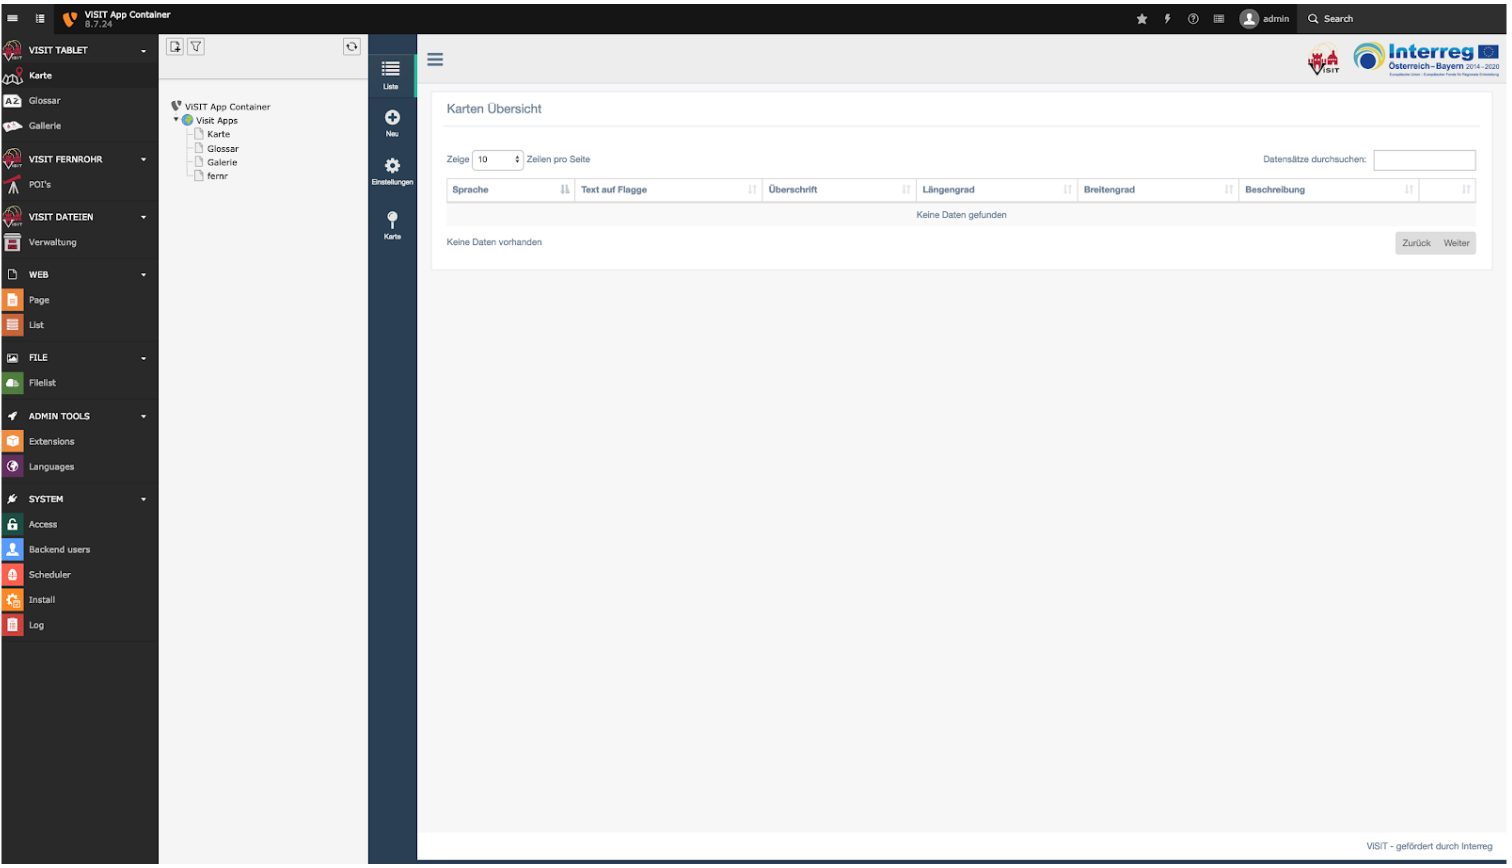
\includegraphics[width=12cm]{Figures/paula/karte/kartenapp.png}
\caption{Leere Kartenübersicht}
\label{img:kartenapp}
\end{figure}

\subsection{Erstellung der Startseite für die Karten-Applikation}

Dazu in der dunkelblauen Leiste “Einstellungen” auswählen (siehe Abbildung \ref{img:startseite_karte}).

\begin{figure}[ht!]
\centering
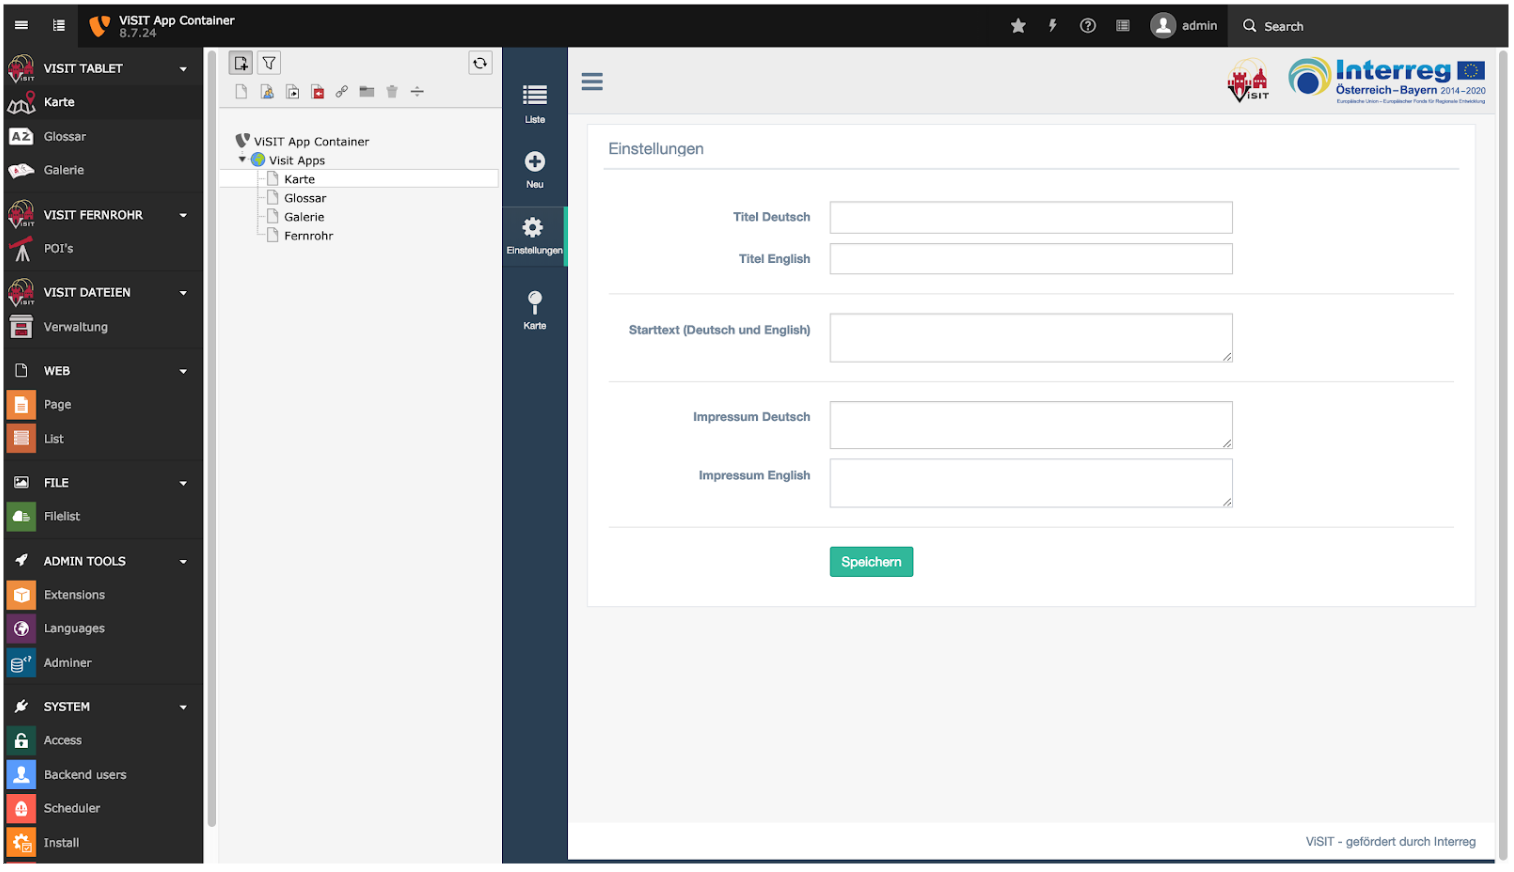
\includegraphics[width=12cm]{Figures/paula/karte/startseite_karte.png}
\caption{Erstellung der Startseite für die Karten-Applikation}
\label{img:startseite_karte}
\end{figure}

Die Startseite wird dem Besucher als erstes angezeigt, auf dieser kann der Besucher die gewünschte Sprache auswählen. Damit das Design des Textes immer gleich aussieht, gibt es unter \url{https://github.com/ViSIT-Dev/appbundle} in der README.md ein Beispiel für die Startseite der Tablets (siehe Abbildung \ref{img:github_link}).\\

\begin{figure}[ht!]
\centering
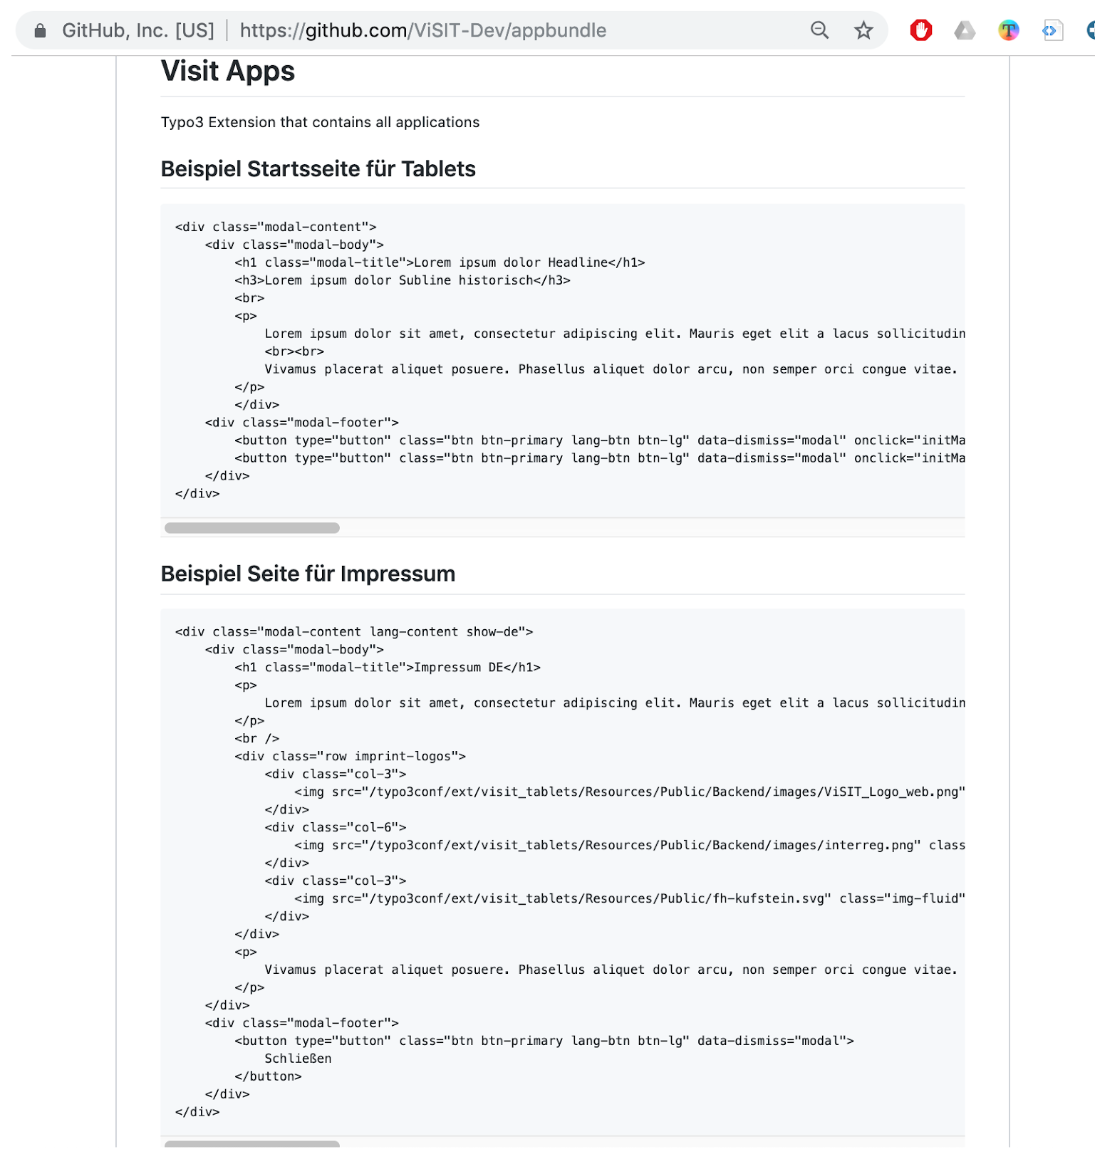
\includegraphics[width=12cm]{Figures/paula/karte/github_link.png}
\caption{Text für die Startseite der Applikationen, zu finden auf \url{https://github.com/ViSIT-Dev/appbundle}}
\label{img:github_link}
\end{figure}

Für jede Sprache wird ein Titel sowie der Impressumstext benötigt. Jetzt werden die beiden Texte aus der zuvor genannten Github-Seite benötigt (siehe Abbildung \ref{img:github_link}). Der erste Text ist der Starttext, dieser beinhaltet die HTML-Elemente Überschrift, Paragraph und Buttons über welche die gewünschte Sprache gewählt werden kann. Die einzelnen Texte in den Tags können mit dem gewünschten Text überschrieben werden (siehe Abbildung \ref{img:befuellte_startseite_karte}).\\

Wenn weitere Sprachen außer Deutsch und Englisch verfügbar sind, können weitere Sprachauswahl-Buttons durch das Markieren des gesamten <button>-Tags ausgewählt werden, dann kopieren und darunter einfügen, erstellt werden. Zwei Sachen müssen beachtet werden: einerseits muss in der \textit{onclick=\glqq initMap('...')\grqq{}}-Methode die der Sprache entsprechende ID eingegeben werden und für den Button der Pfad für die Flagge im Image-Tag angegeben werden. Dazu muss zuvor das benötigte Flaggen-Icon, vorzugsweise im PNG-Format, im entsprechenden Ordner gespeichert werden und der Pfad angepasst werden\\ \textit{src=\glqq/typo3/sysext/core/Resources/Public/Icons/Flags/PNG/DE.png\grqq{}}. 

\begin{figure}[ht!]
\centering
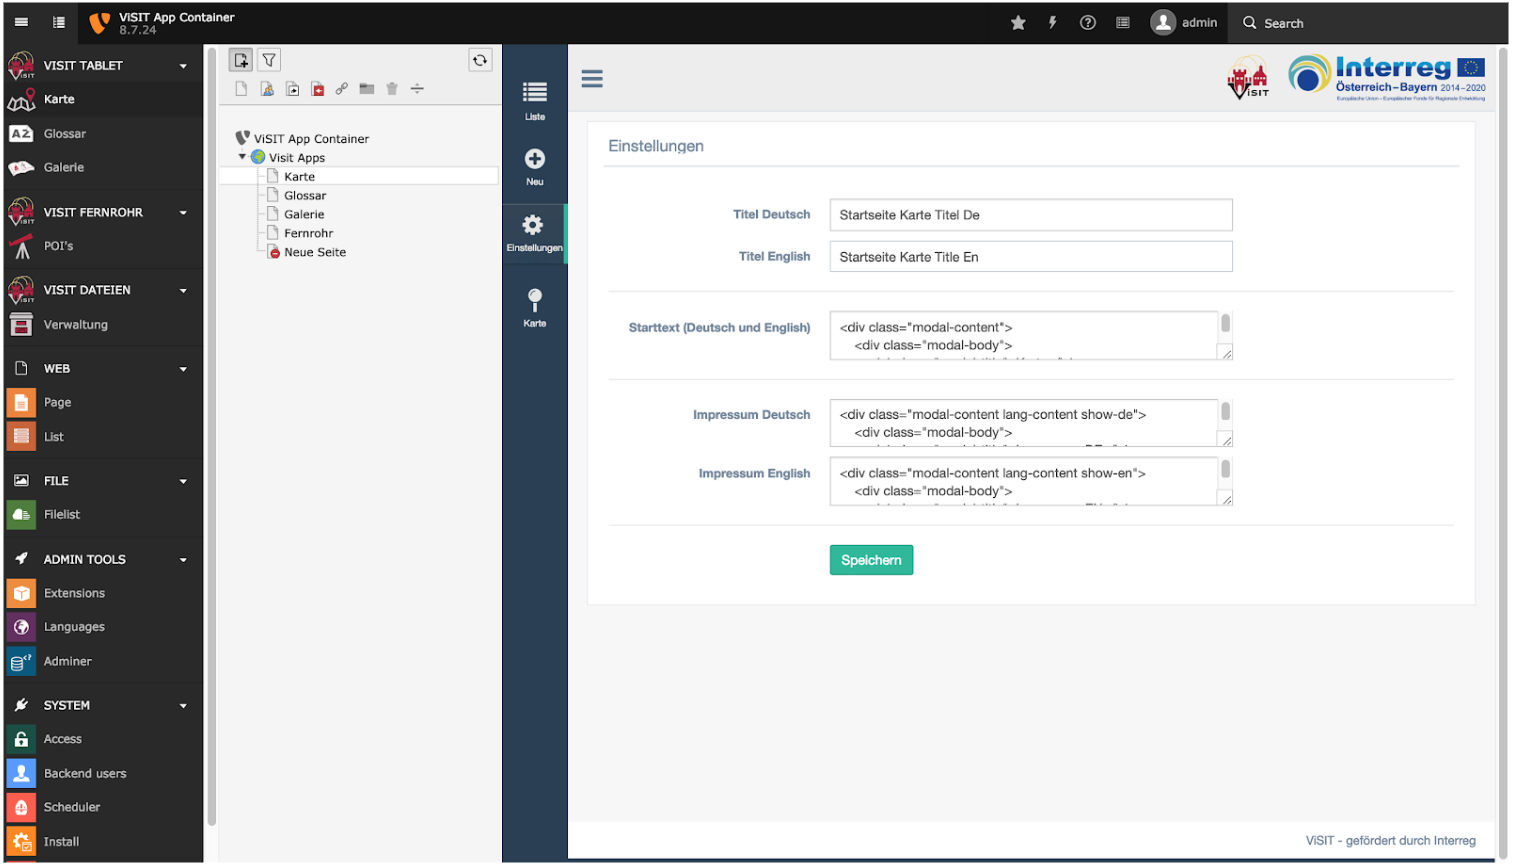
\includegraphics[width=12cm]{Figures/paula/karte/befuellte_startseite_karte.png}
\caption{Erstellung der Startseite für die Karten-Applikation}
\label{img:befuellte_startseite_karte}
\end{figure}

\subsection{Neues Kartenelement hinzufügen}

Mit einem Klick auf \glqq Neu\grqq{} kann ein neues Kartenelement - Point of Interest - hinzugefügt werden (siehe Abbildung \ref{img:neues_kartenelement_hinzufuegen}).

\begin{figure}[ht!]
\centering
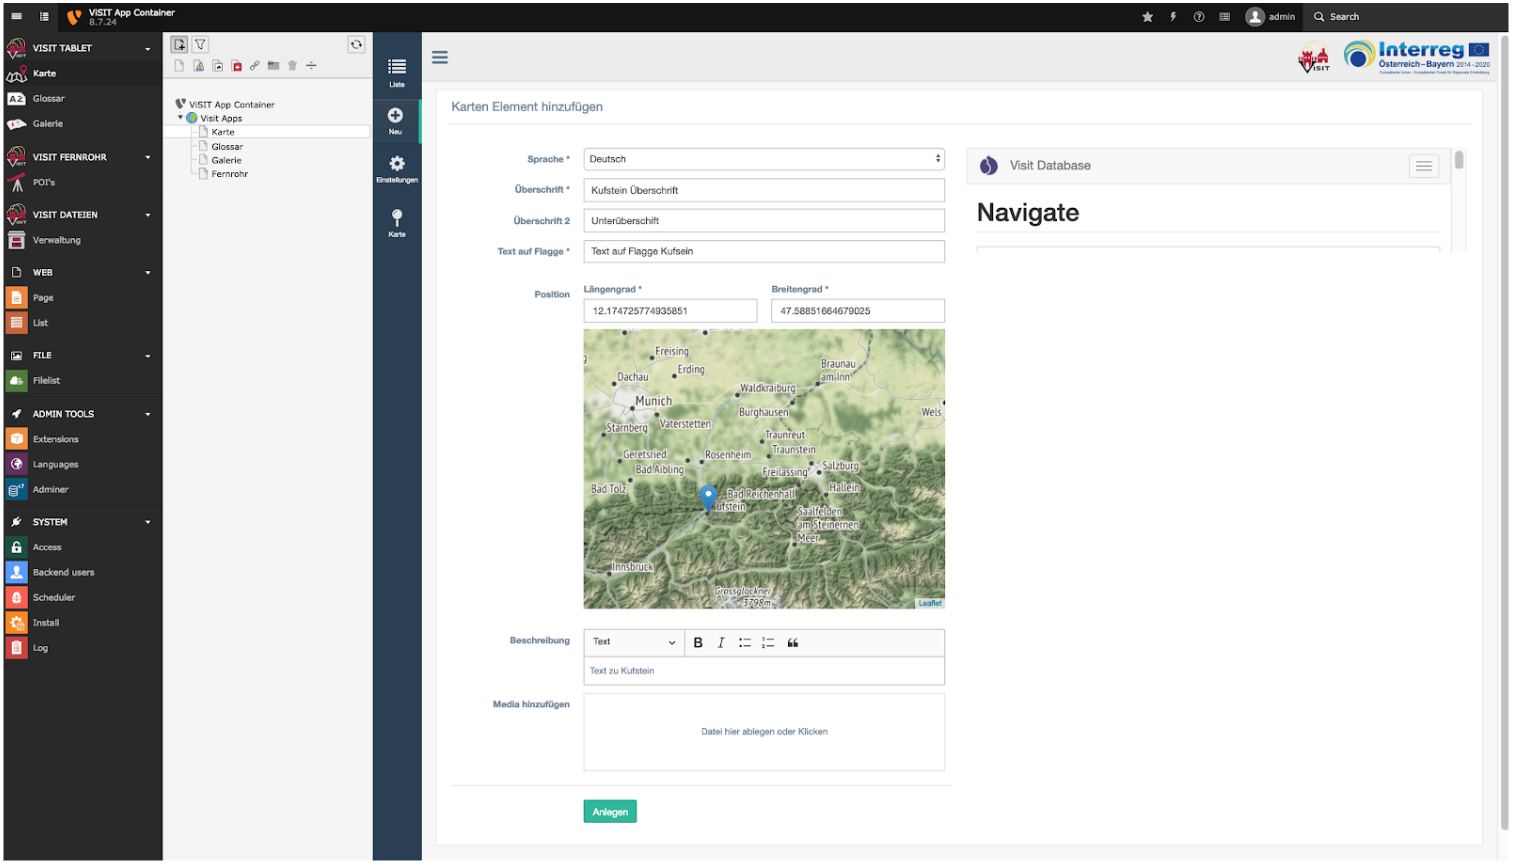
\includegraphics[width=12cm]{Figures/paula/karte/neues_kartenelement_hinzufuegen.png}
\caption{Ein neues Kartenelement hinzufügen}
\label{img:neues_kartenelement_hinzufuegen}
\end{figure}

Ein neues Kartenelement - Point of Interest - benötigt eine Überschrift, eine Unterüberschrift ist optional, einen Text auf der Flagge und eine Beschreibung. Optional können auch weitere Medien hinzugefügt werden. Die geografische Position kann entweder über den Längen- und Breitengrad manuell eingetippt werden oder mittels setzen der Stecknadel auf die Karte, dann werden die Längen- und Breitengrade dieser Stecknadel übernommen. Ist alles vollständig ausgefüllt, kann die Eingabe mit \glqq Anlegen\grqq{} am Seitenende gespeichert werden. Nach dem Klick gelangt man zu der Kartenübersicht, wo alle eingefügten Elemente angeführt sind, jedes dieser Elemente kann sowohl nochmals bearbeitet oder auch wieder gelöscht werden.\\

Klickt man im Seitenbaum mit der rechten Maustaste auf Karte, dann können die angelegten Kartenelemente im Browser angesehen werden.\\
Jedes Kartenelement muss sowohl auf Deutsch als auch auf Englisch angelegt werden (siehe Abbildung \ref{img:listenuebersicht_kartenelemente}).

\begin{figure}[ht!]
\centering
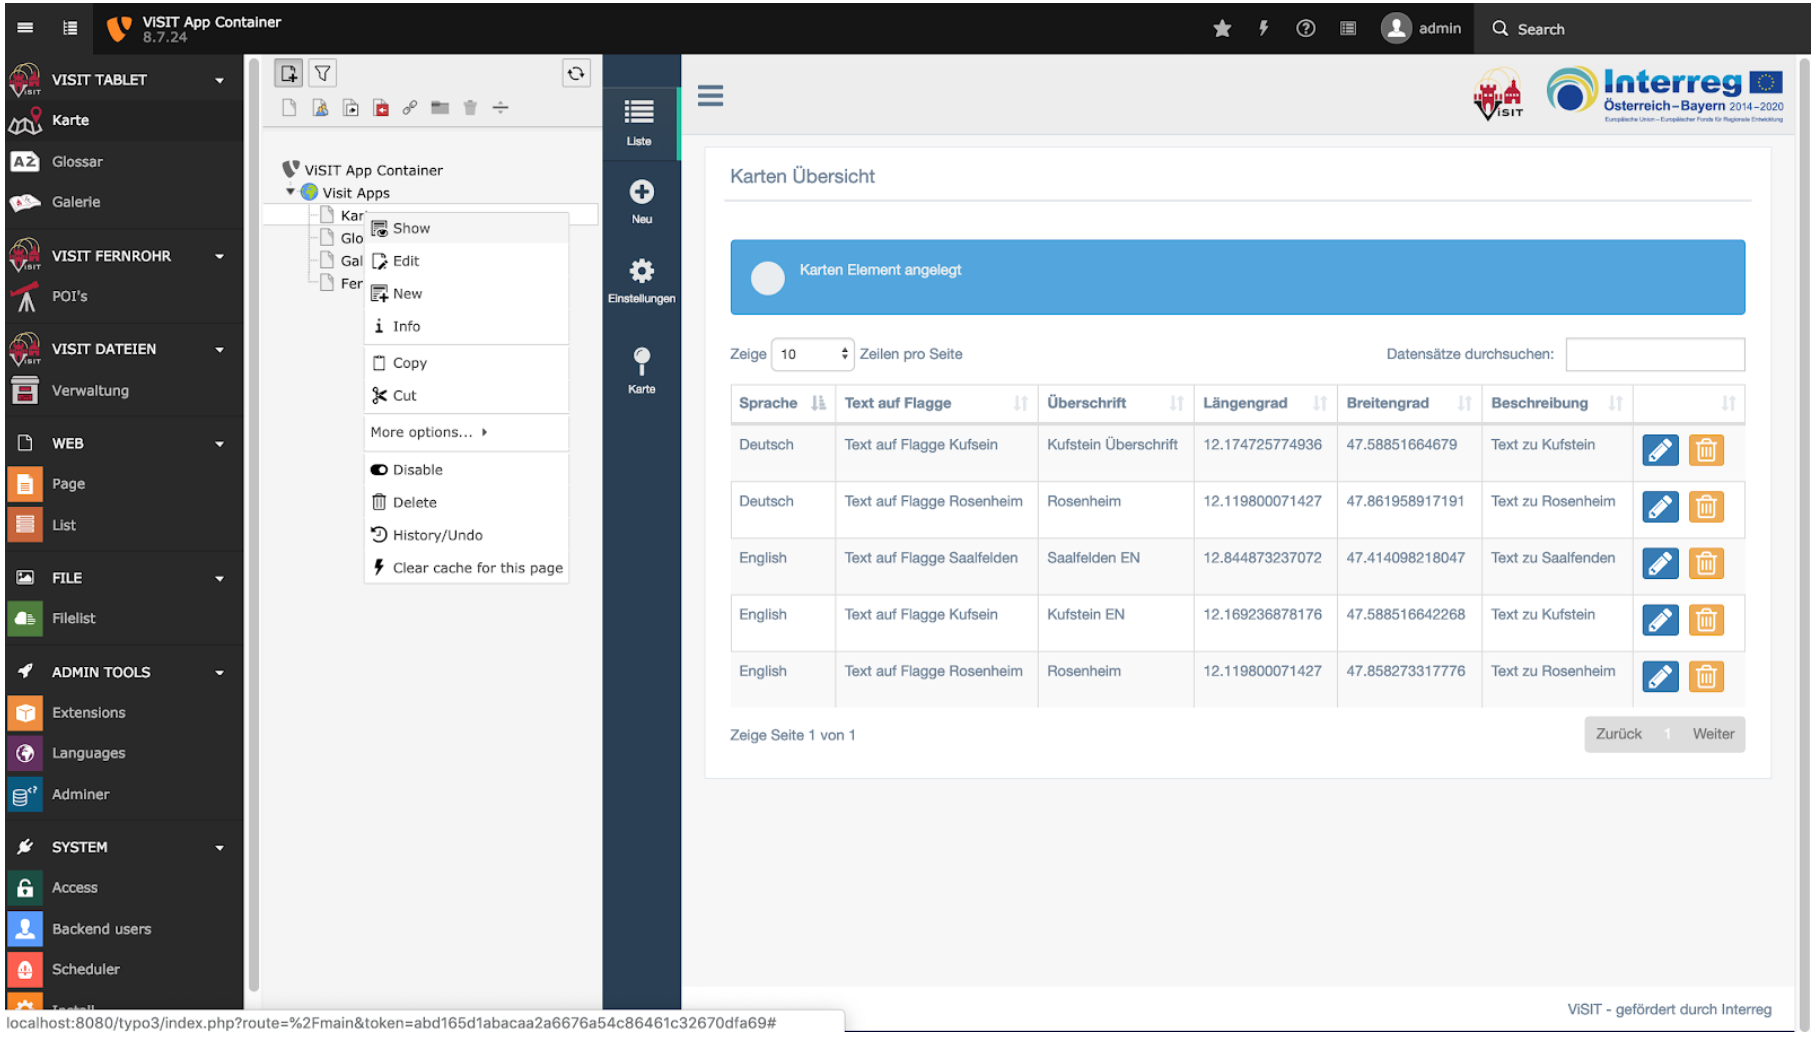
\includegraphics[width=12cm]{Figures/paula/karte/listenuebersicht_kartenelemente.png}
\caption{Listenansicht über alle angelegten Kartenelemente}
\label{img:listenuebersicht_kartenelemente}
\end{figure}

Dabei wird zuerst die Startseite angezeigt, auf welcher der Besucher seine Sprache wählen kann (siehe Abbildung \ref{img:startseite_kartenapp}).

\begin{figure}[ht!]
\centering
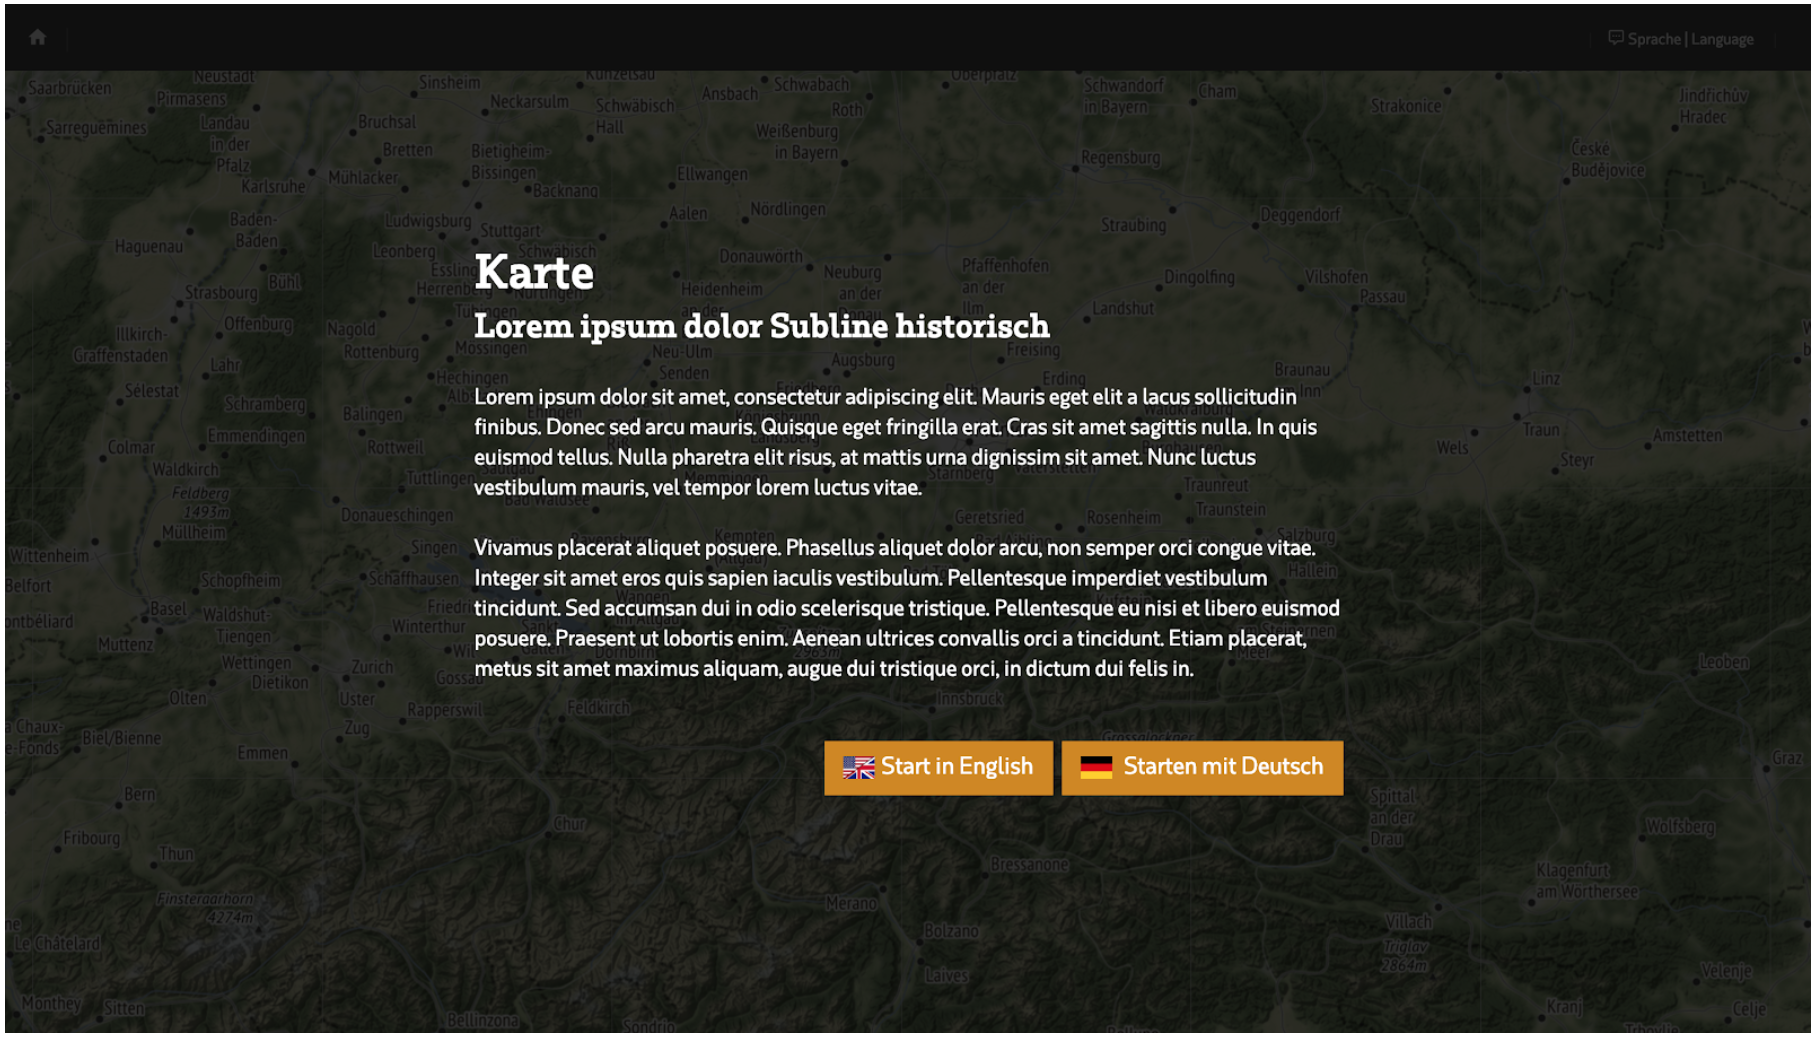
\includegraphics[width=12cm]{Figures/paula/karte/startseite_kartenapp.png}
\caption{Startseite der Karten-Applikation}
\label{img:startseite_kartenapp}
\end{figure}

Nach der Auswahl der Sprache wird dem Besucher die Karte mit den einzelnen Kartenelementen - Point of Interest - auf dem Tablet angezeigt (siehe Abbildung \ref{img:karte_browser}).

\begin{figure}[ht!]
\centering
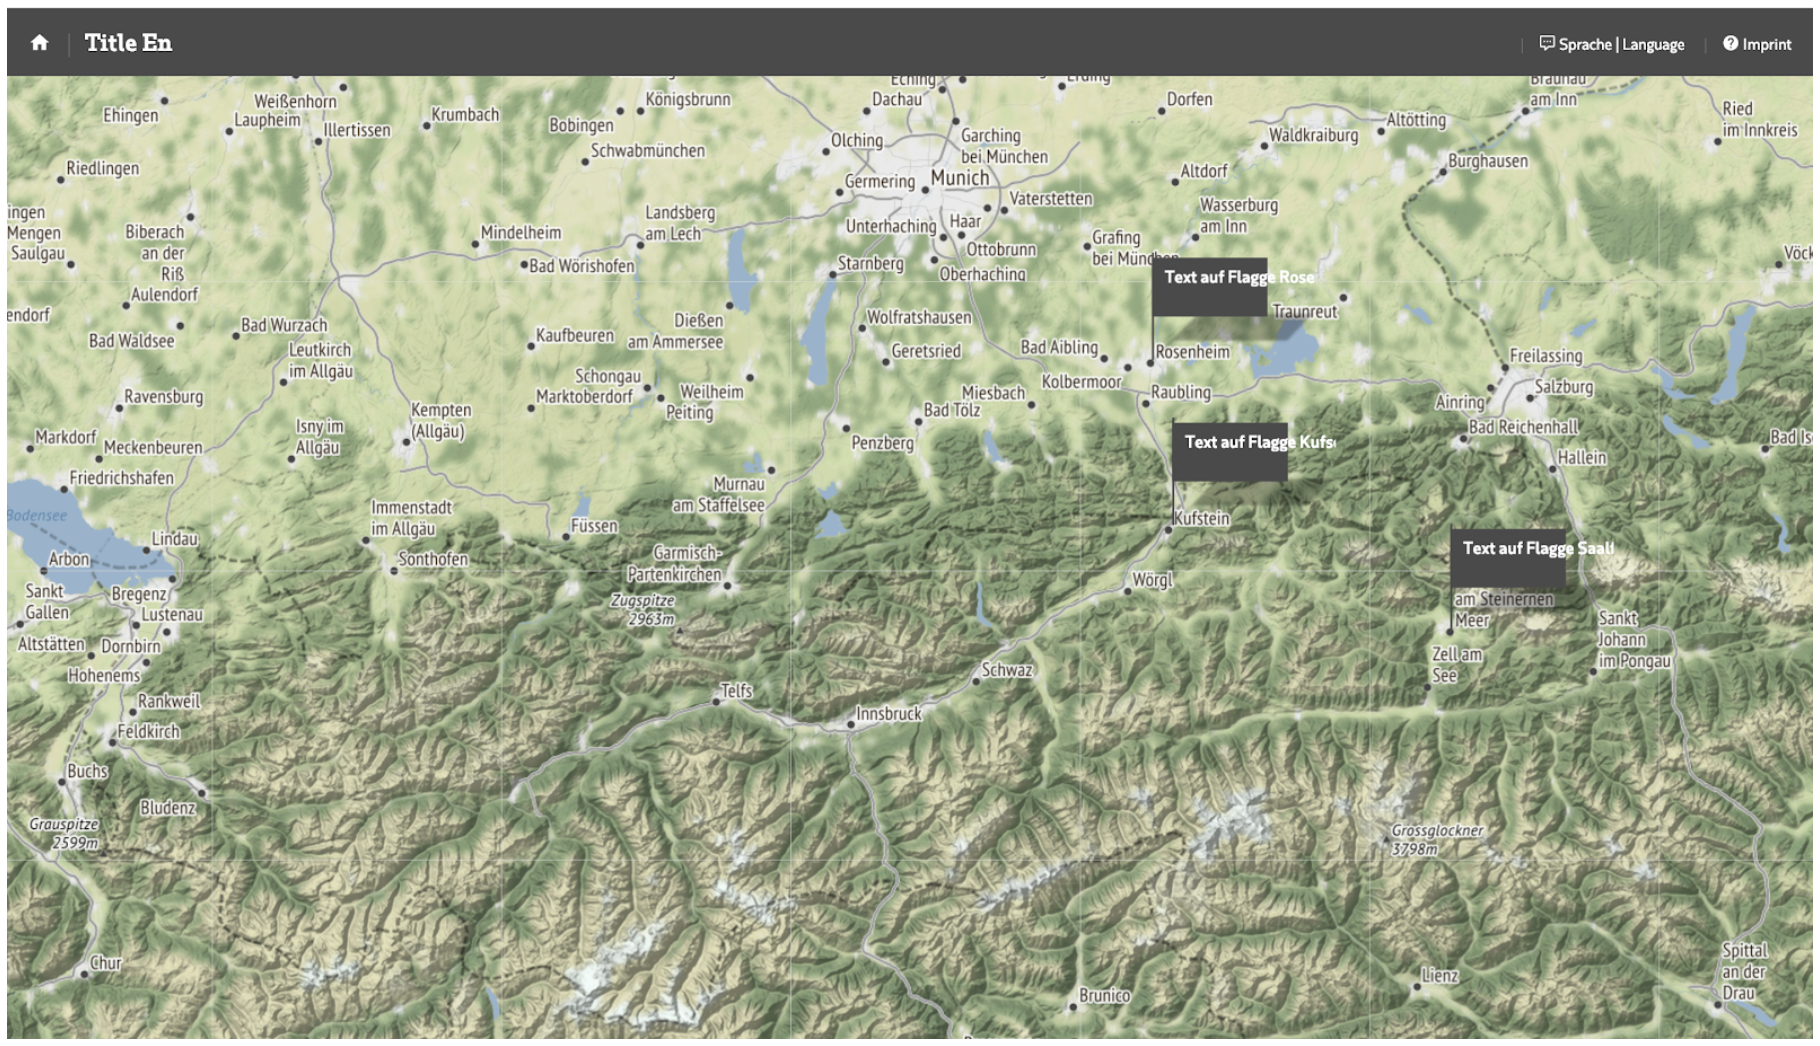
\includegraphics[width=12cm]{Figures/paula/karte/karte_browser.png}
\caption{Ansicht der Karte im Browser}
\label{img:karte_browser}
\end{figure}

Jetzt kann der Besucher eine Flagge auswählen, zu welcher er mehr Informationen haben möchte und via Klick öffnet sich der seitliche Infobereich auf der rechten Seite (siehe Abbildung \ref{img:kartenelement_detail}).

\begin{figure}[ht!]
\centering
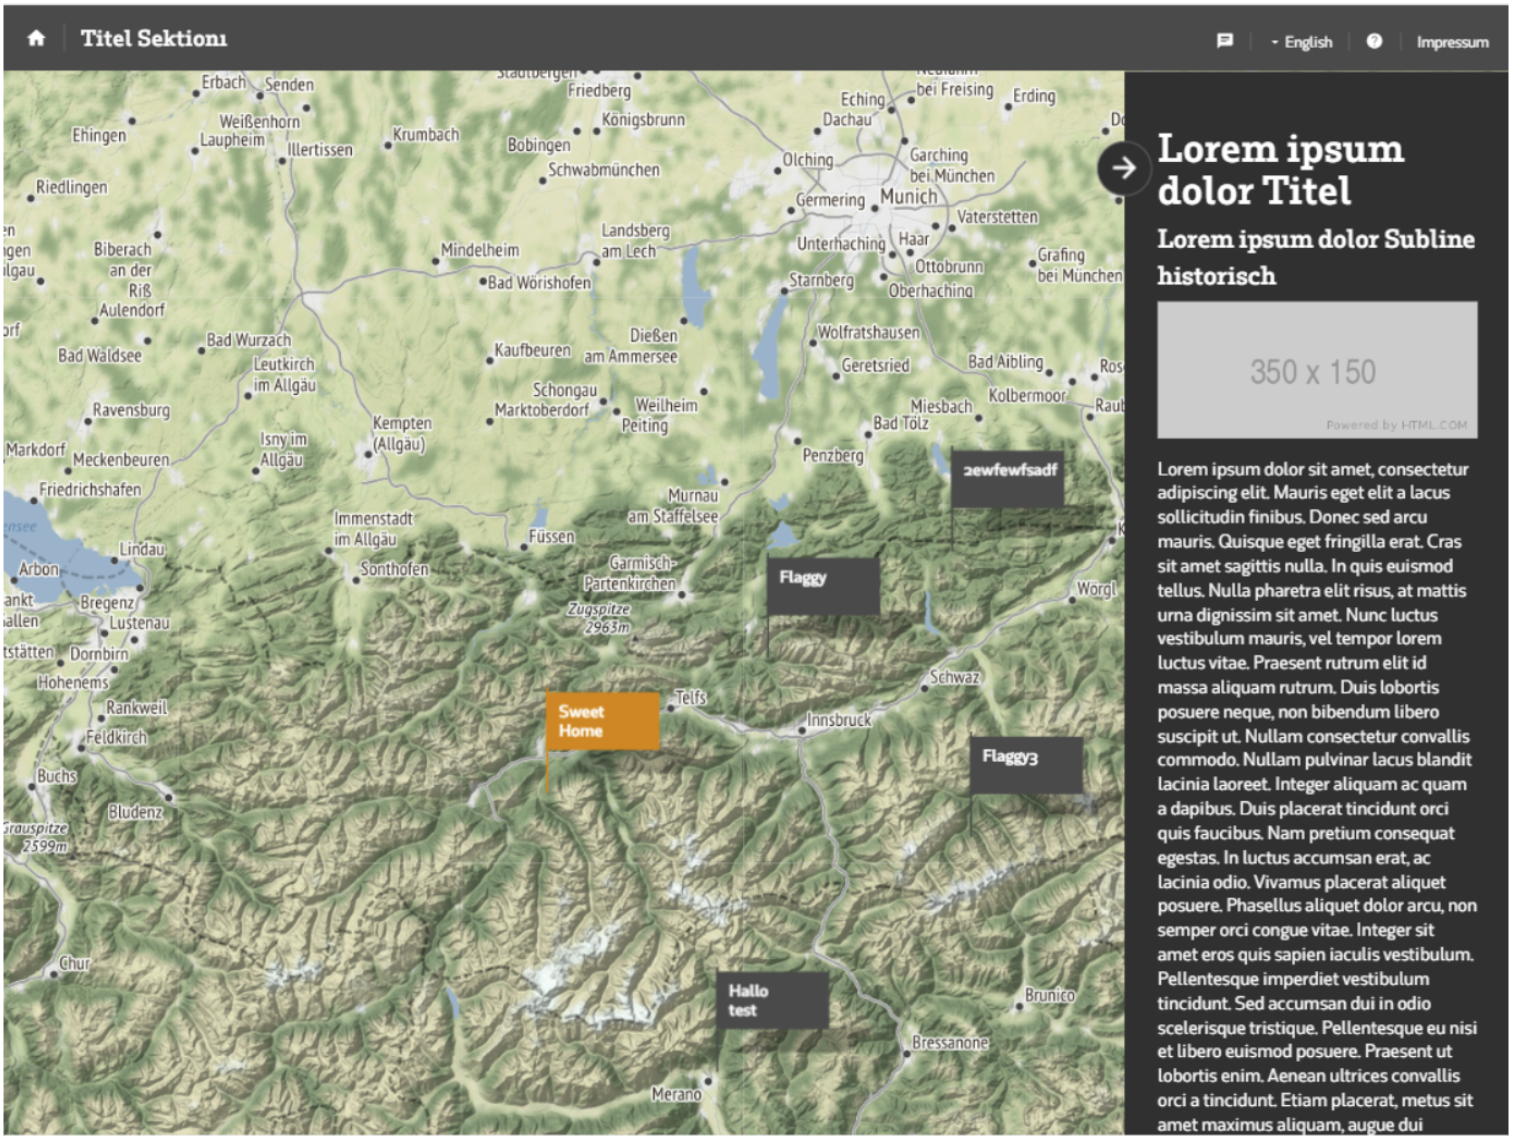
\includegraphics[width=12cm]{Figures/paula/karte/kartenelement_detail.png}
\caption{Kartenelement - Point of Interest - mit Detailinformation}
\label{img:kartenelement_detail}
\end{figure}

\subsection{Bearbeitung und Löschen von angelegten Kartenelementen}

Die Kartenelemente können jederzeit bearbeitet oder gelöscht werden. Dies geht indem zuerst die Listenansicht in der dunkelblauen Leiste ausgewählt wird. In weiterer Folge kann jedes einzelne Element (Zeile) einzeln bearbeitet oder gelöscht werden. Zum Bearbeiten auf das blaue Stiftsymbol auf der rechten Seite klicken, zum Löschen des Objekts, den orangen Müllkübel.




\cleardoublepage

\section{Glossar-Applikation}

In der Glossar-Applikation werden Insassen des Gefängnisses aufgelistet. Die Applikation ist in zwei Bereiche aufgeteilt, links werden die Insassen aufgelistet und rechts wird der Inhalt zu dem Insassen dargestellt. Wählt der Benutzer einen Namen aus dieser Liste aus, so werden die Details zu dieser Person in der rechten Spalte angezeigt. Die Auflistung der Insassen erfolgt alphabetisch nach Vornamen beziehungsweise, wenn vorhanden, nach dem Nachnamen (siehe Abbildung \ref{img:glossar}).
Die Auflistung kann auch nach Ereignis, Zelle oder VIP erfolgen, dies kann der Besucher in der oberen Menüzeile auswählen.

\begin{figure}[ht!]
\centering
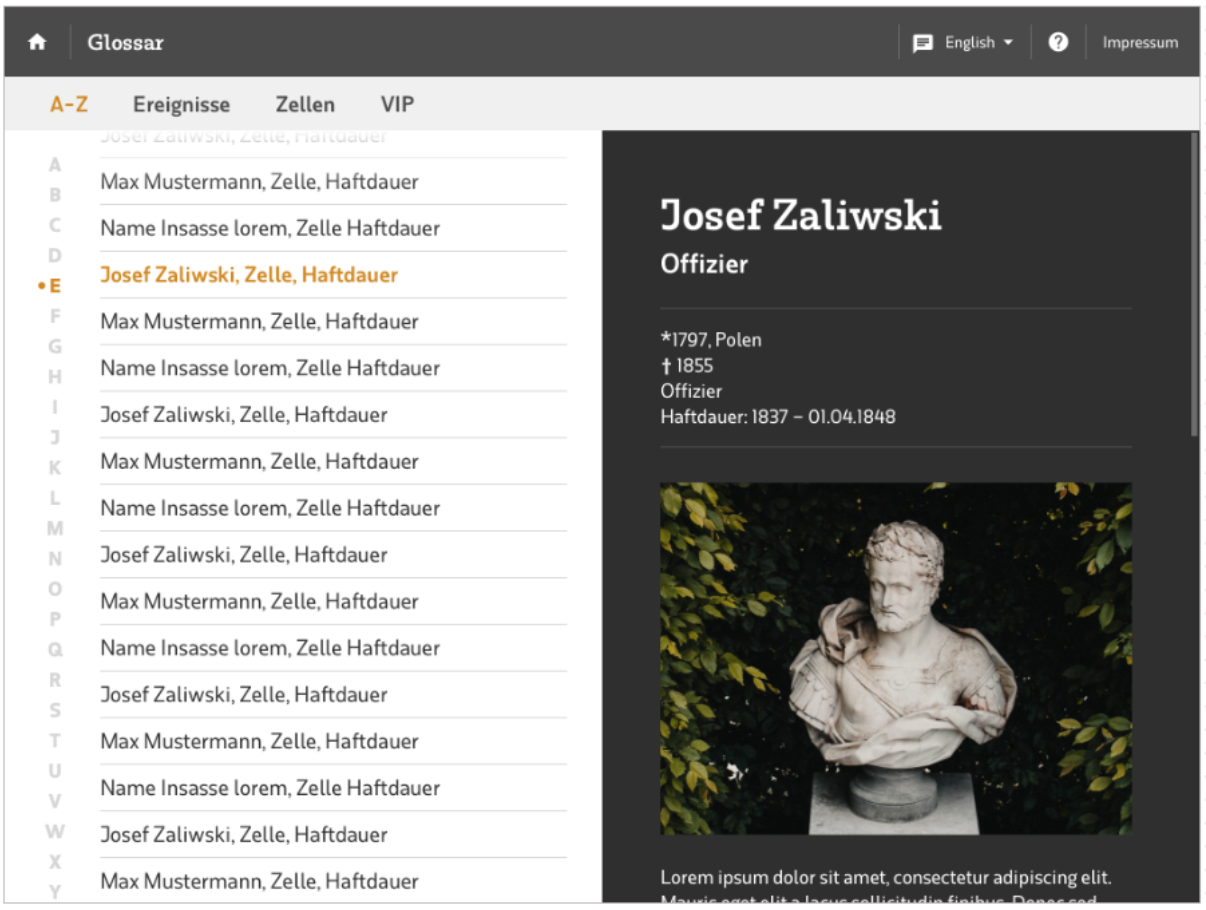
\includegraphics[width=12cm]{Figures/paula/glossar/glossar_anfang.png}
\caption{Ansicht der Glossar-Applikation auf einem Tablet}
\label{img:glossar}
\end{figure}


\subsection{Einpflegen der Daten in die Glossar-Applikation}

Dazu aus der Modulleiste links unter der Obergruppe VISIT TABLET das Glossar auswählen. Im linken Teil des Hauptfensters ist der Seitenbaum zu sehen und rechts befindet sich die Insassen-Übersicht (siehe Abbildung \ref{img:uebersicht_glossar}).

\begin{figure}[ht!]
\centering
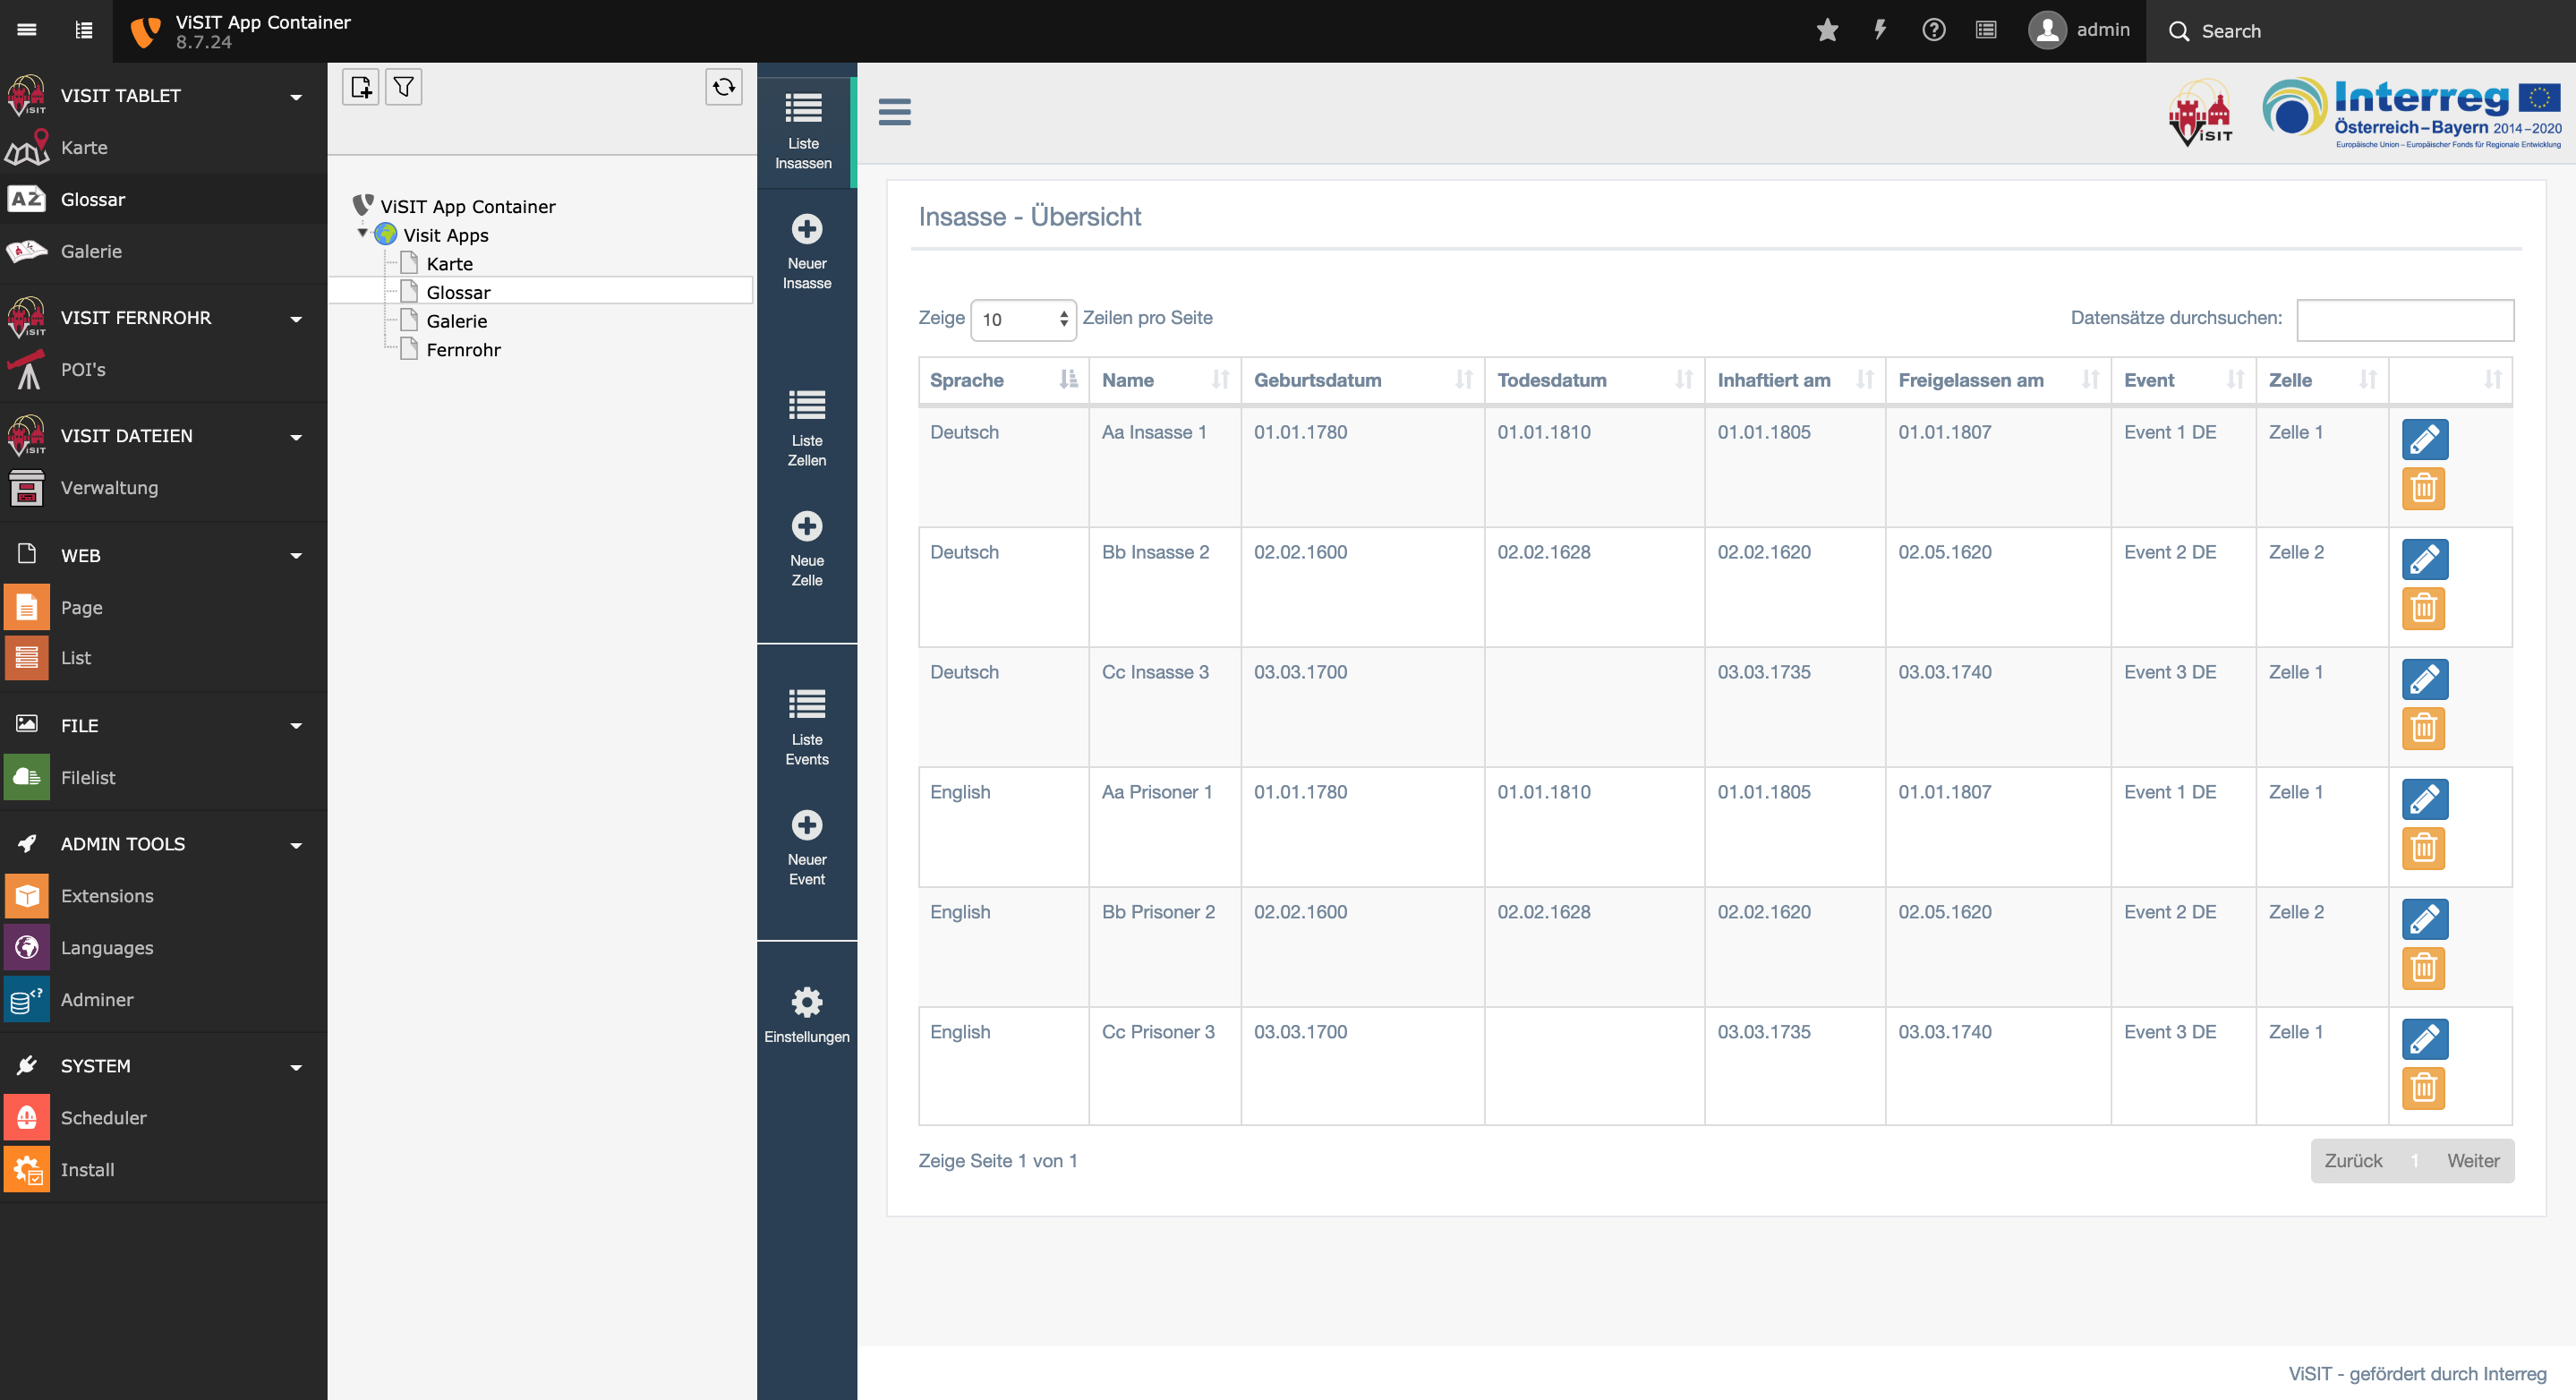
\includegraphics[width=12cm]{Figures/paula/glossar/uebersicht_insassen.png}
\caption{Übersicht über alle angelegten Insassen}
\label{img:uebersicht_glossar}
\end{figure}


\subsection{Erstellung der Startseite für die Glossar-Applikation}

Das Glossar kann mit einem Klick auf \glqq Glossar\grqq{} in der Modulleiste konfiguriert werden (siehe Abbildung \ref{img:konfiguration_glossar}).

\begin{figure}[ht!]
\centering
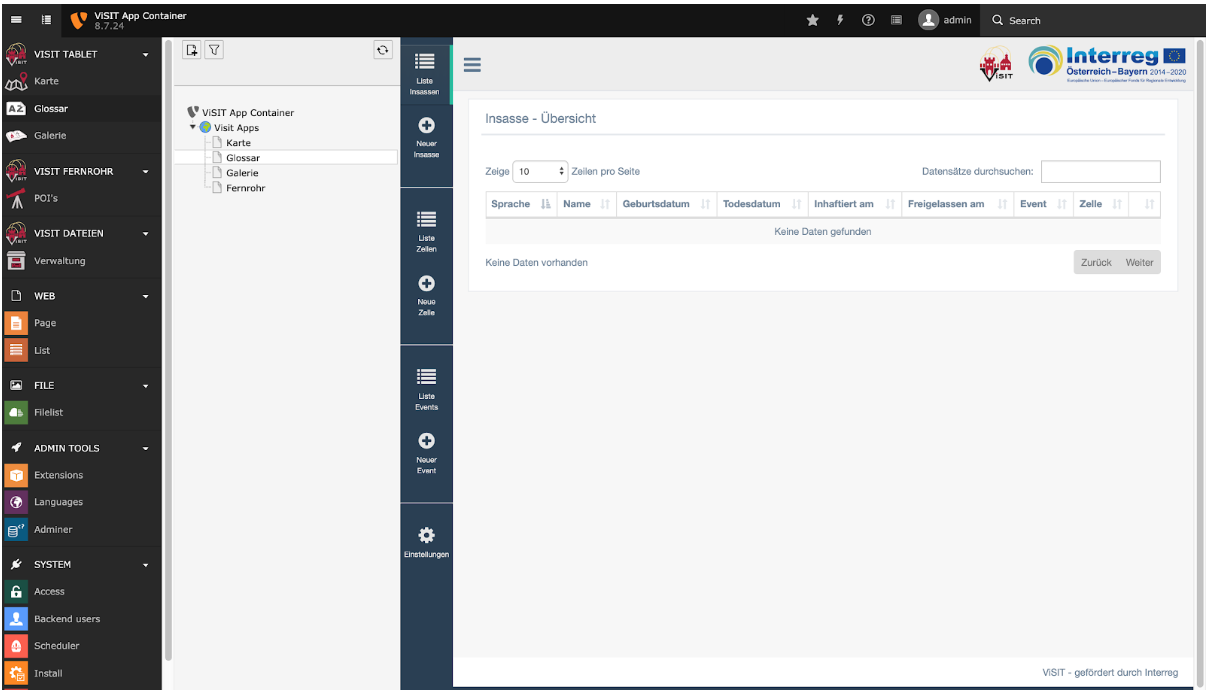
\includegraphics[width=12cm]{Figures/paula/glossar/konfiguration_glossar.png}
\caption{Konfiguration der Glossar-Applikation}
\label{img:konfiguration_glossar}
\end{figure}

Die Startseite der Applikation kann unter \glqq Einstellungen\grqq{} in der dunkelblauen Leiste konfiguriert werden. Dafür benötigt man den Text für die Startseite \url{https://github.com/ViSIT-Dev/appbundle}. Dieser Text muss in die entsprechenden Inputfelder kopiert werden (siehe Abbildung \ref{img:startseite_glossar}).

\begin{figure}[ht!]
\centering
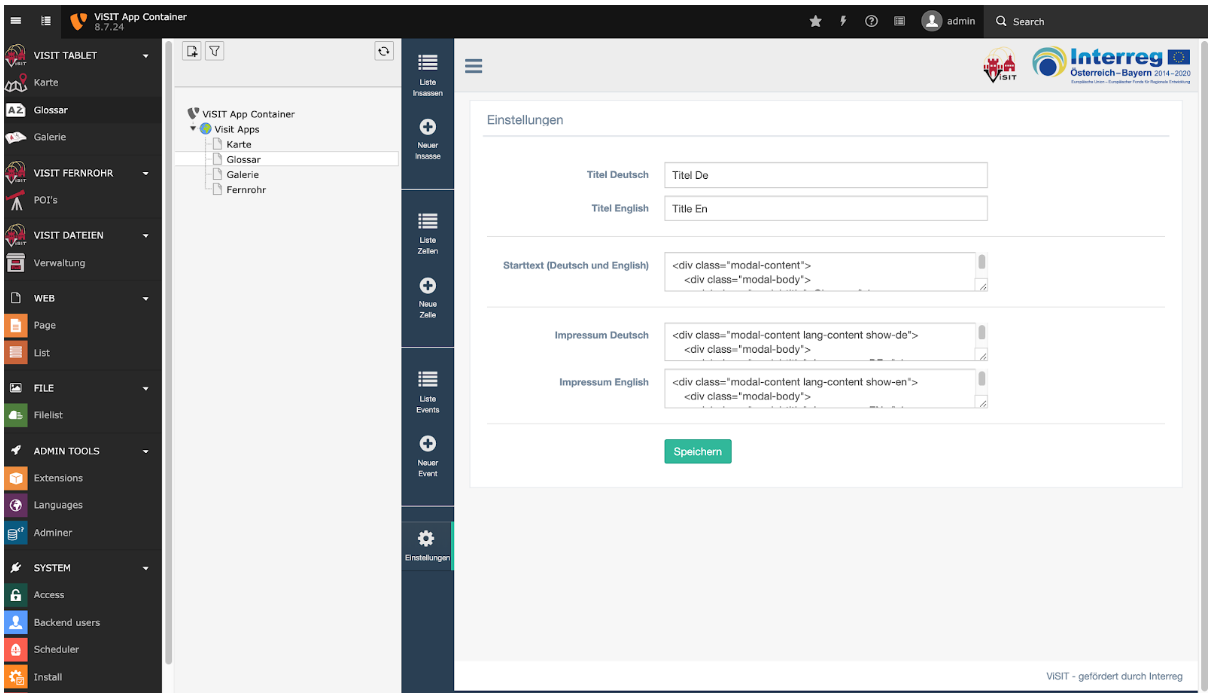
\includegraphics[width=12cm]{Figures/paula/glossar/startseite_glossar.png}
\caption{Befüllung der Startseite der Glossar-Applikation}
\label{img:startseite_glossar}
\end{figure}

Nachdem die Startseite befüllt wurde, wird sie dem Besucher als erstes angezeigt, auf dieser kann der Besucher dann die gewünschte Sprache auswählen (siehe Abbildung \ref{img:startseite_glossar_tablet}).

\begin{figure}[ht!]
\centering
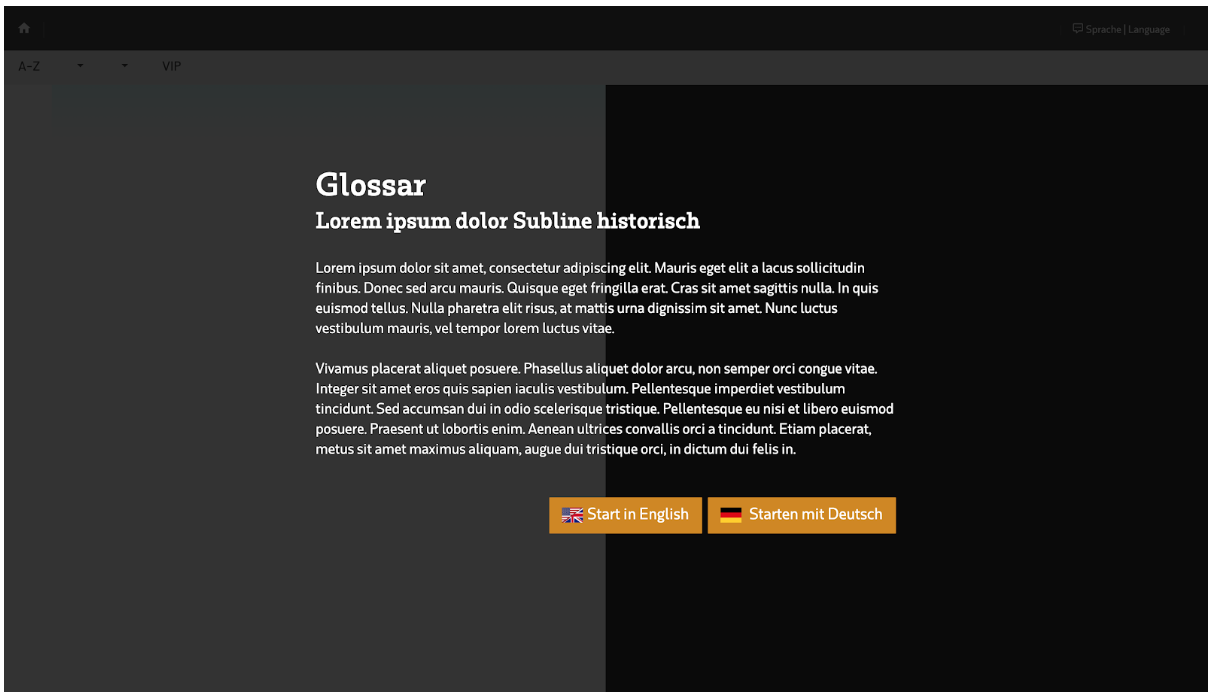
\includegraphics[width=12cm]{Figures/paula/glossar/startseite_glossar_tablet.png}
\caption{Startseite der Glossar-Applikation}
\label{img:startseite_glossar_tablet}
\end{figure}


\subsection{Neue Zelle hinzufügen}

Über einen Klick auf \glqq Neue Zelle\grqq{} in der dunkelblauen Leiste kann eine neue Zelle angelegt werden (siehe Abbildung \ref{img:hinzufuegen_neue_zelle}).

\begin{figure}[ht!]
\centering
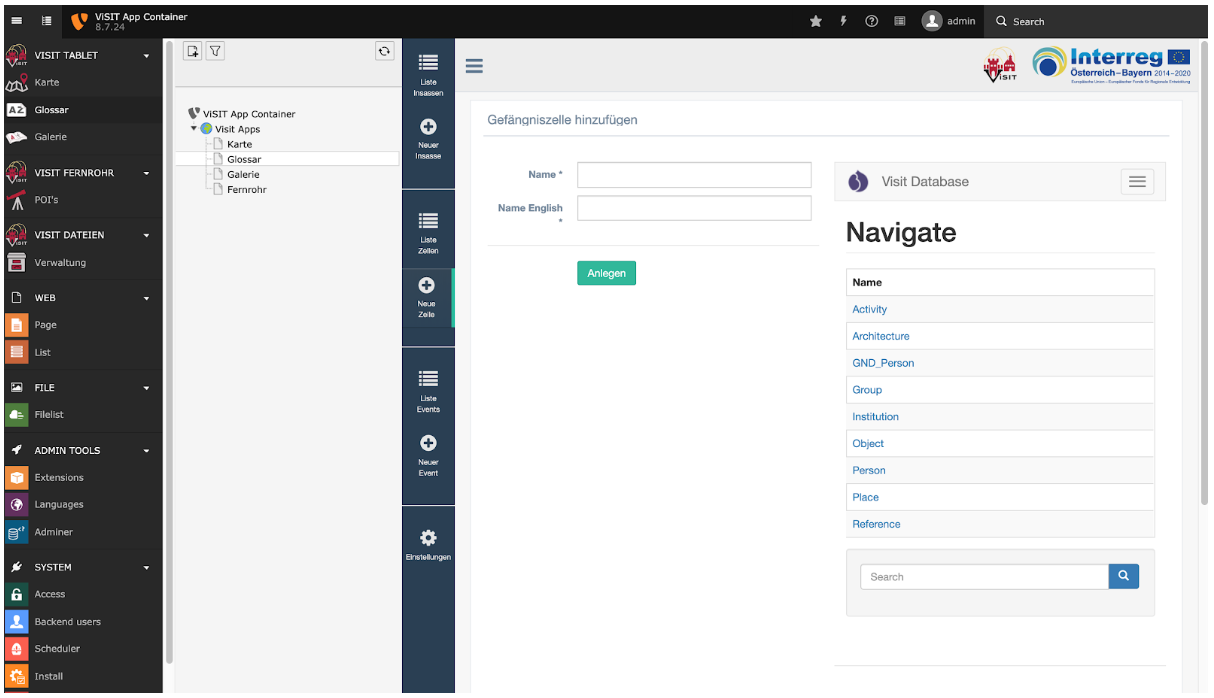
\includegraphics[width=12cm]{Figures/paula/glossar/hinzufuegen_neue_zelle.png}
\caption{Hinzufügen einer neuen Zelle}
\label{img:hinzufuegen_neue_zelle}
\end{figure}

Die Zelle benötigt sowohl einen deutschen als auch englischen Zellennamen. Mit einem Klick auf \glqq Anlegen\grqq{}, werden die eingegebenen Daten dauerhaft gespeichert. 

\begin{figure}[ht!]
\centering
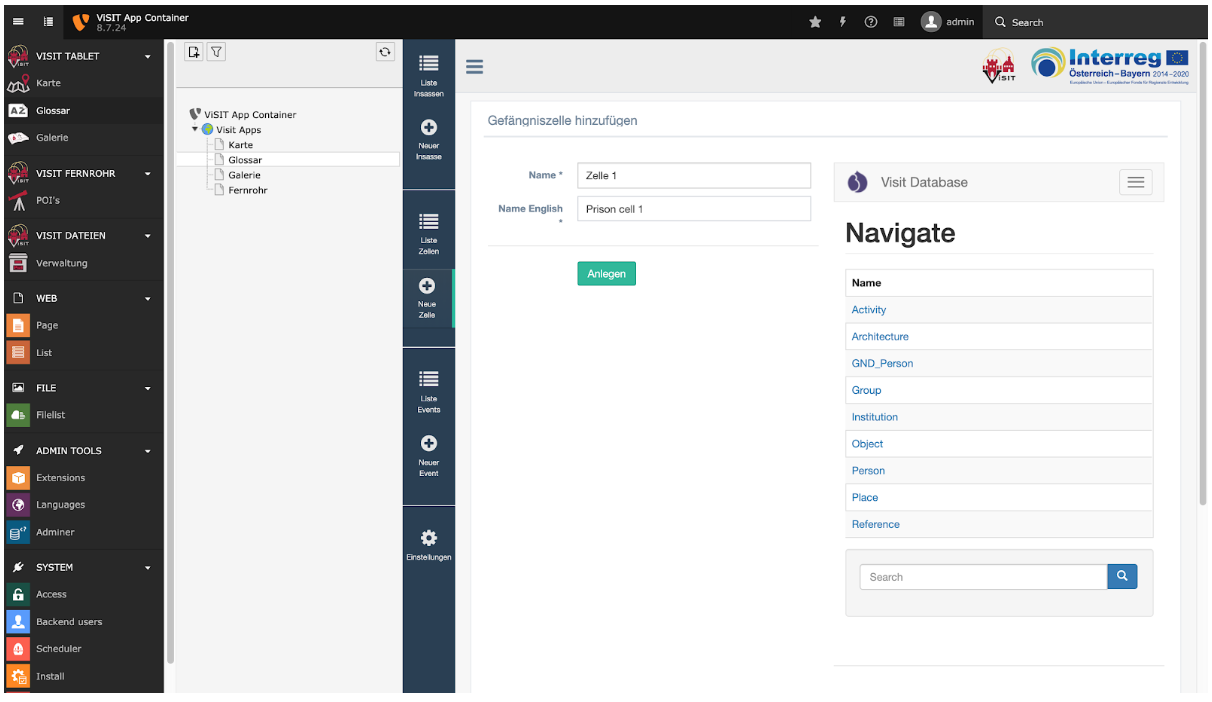
\includegraphics[width=12cm]{Figures/paula/glossar/neue_zelle_erstellen.png}
\caption{Erstellen einer neuen Zelle}
\label{img:neue_zelle}
\end{figure}

Alle angelegten Zellen können über \glqq Liste Zellen\grqq{} in der dunkelblauen Leiste angesehen werden (siehe Abbildung \ref{img:angelegte_zellen}).

\begin{figure}[ht!]
\centering
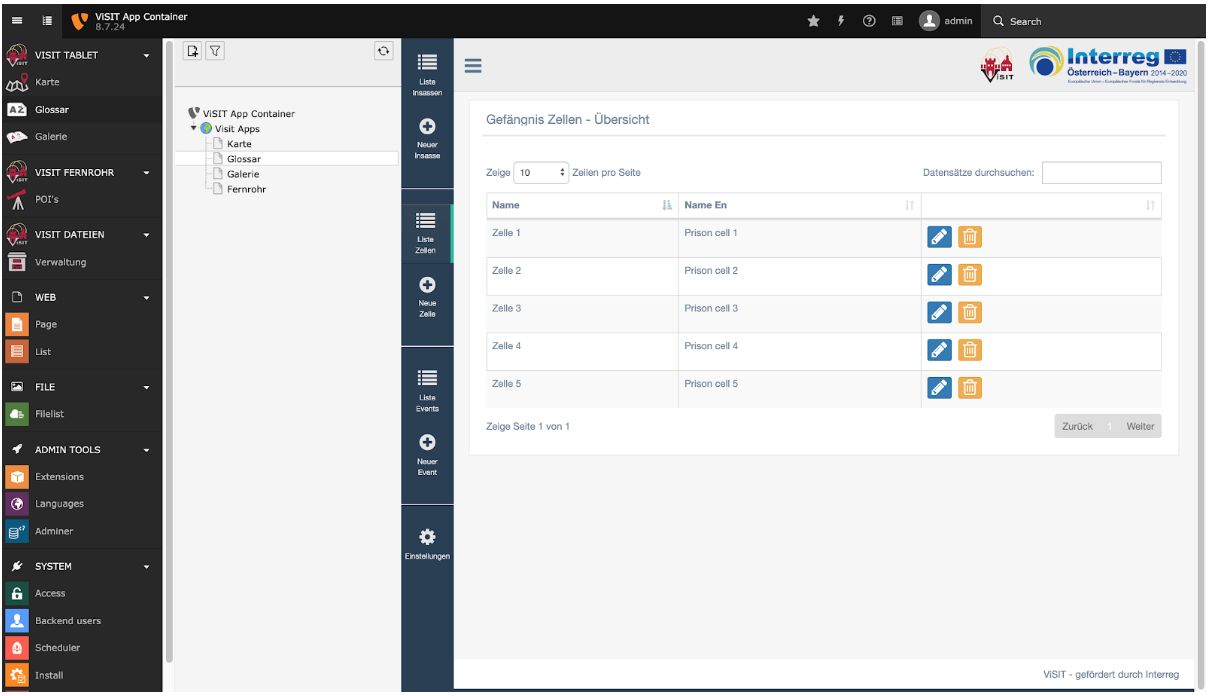
\includegraphics[width=12cm]{Figures/paula/glossar/angelegte_zellen.png}
\caption{Angelegte Zellen in der Listenübersicht}
\label{img:angelegte_zellen}
\end{figure}

\subsection{Neuen Event hinzufügen}

Ein Event benötigt ebenfalls einen deutschen und einen englischen Namen, mit einem Klick auf \glqq Anlegen\grqq{} werden die eingegebenen Daten dauerhaft gespeichert \ref{img:hinzufuegen_event}.
\begin{figure}[ht!]
\centering
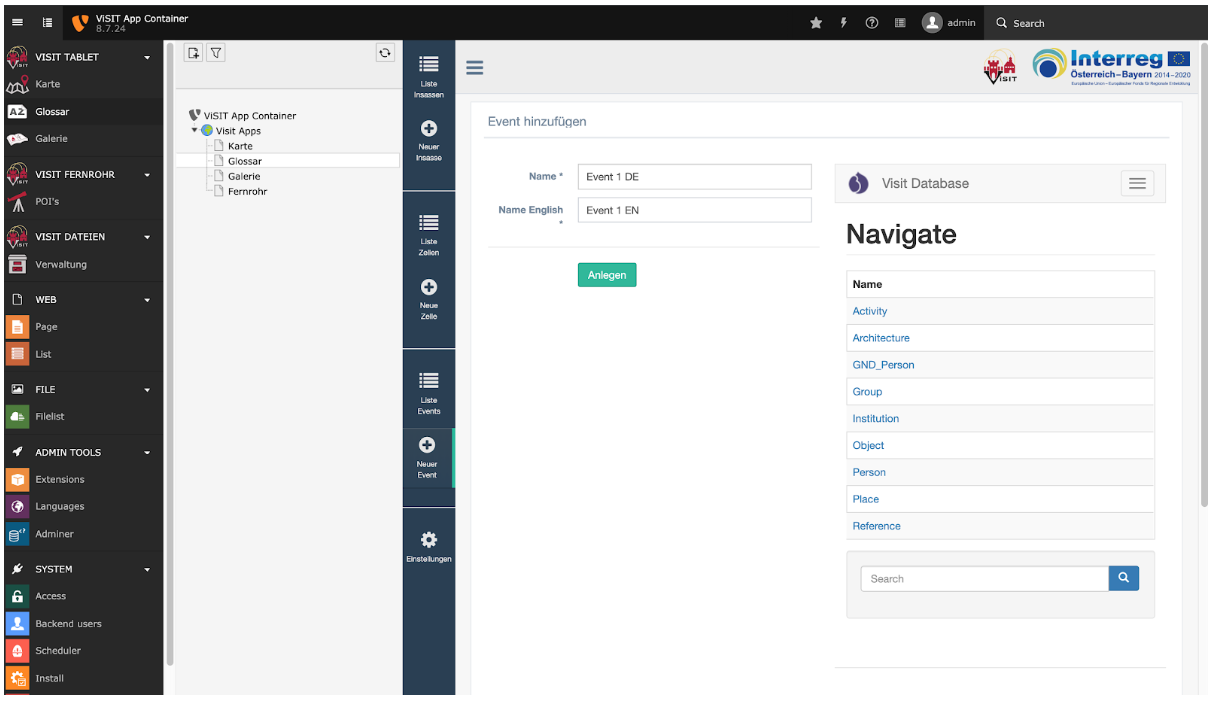
\includegraphics[width=12cm]{Figures/paula/glossar/hinzufuegen_event.png}
\caption{Hinzufügen eines neuen Events}
\label{img:hinzufuegen_event}
\end{figure}

In \glqq Liste Events\grqq{} in der dunkelblauen Leiste können alle Events angezeigt werden.

\begin{figure}[ht!]
\centering
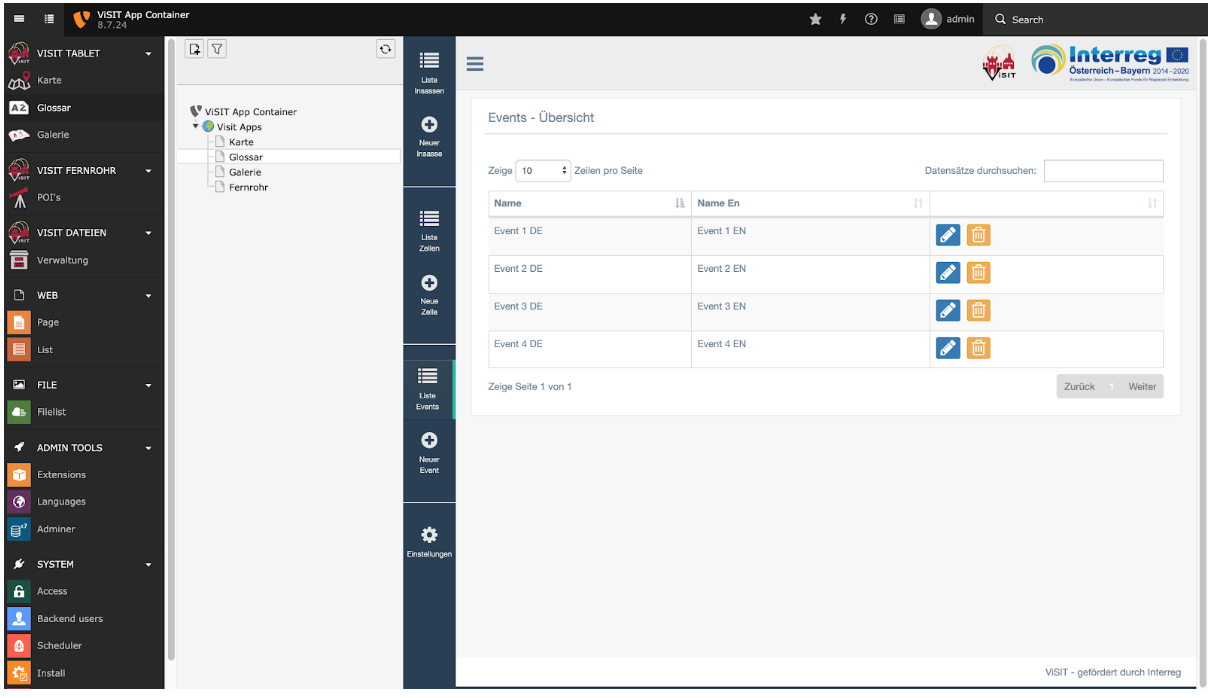
\includegraphics[width=12cm]{Figures/paula/glossar/angelegte_events_listenansicht.png}
\caption{Angelegte Events in der Listenansicht}
\label{img:angelegte_events_listenansicht}
\end{figure}

\subsection{Neuen Insassen hinzufügen}

Über die Auswahl \glqq Neuer Insasse\grqq{} in der dunkelblauen Leiste kann ein neuer Insasse angelegt werden. Die Felder Geburtsdatum, Todestag, Inhafiert sowie Freigelassen sind Datumsfelder. Ist eines der Daten nicht bekannt, kann das Feld freigelassen werden (siehe Abbildung \ref{img:anlegen_insassen}).

\begin{figure}[ht!]
\centering
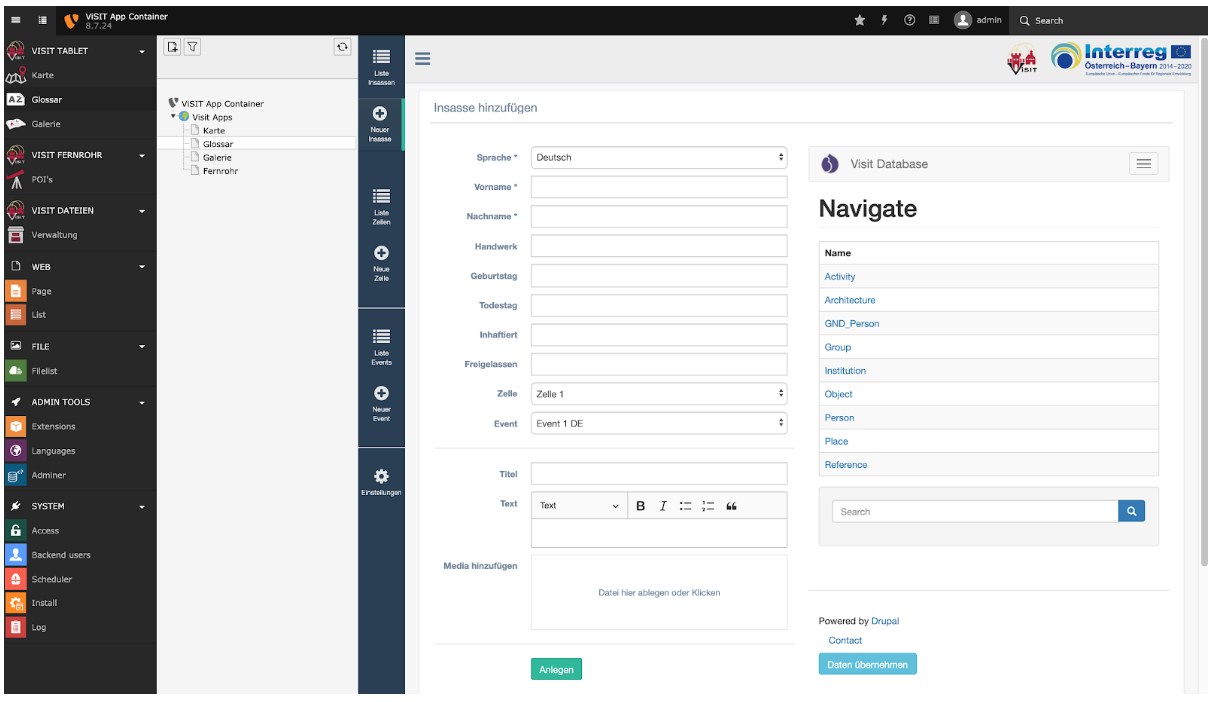
\includegraphics[width=12cm]{Figures/paula/glossar/anlegen_insassen.png}
\caption{Anlegen eines neuen Insassens}
\label{img:anlegen_insassen}
\end{figure}

Legt man einen Insassen an, muss bei Zelle sowie Event eine bereits angelegte Zelle beziehungsweise ein angelegtes Event angegeben werden. Klickt man auf die Pfeile im Inputfeld, so öffnet sich ein Dropdown Menü und hier kann die entsprechende Zelle beziehungsweise das entsprechende Event ausgewählt werden (siehe Abbildung \ref{img:anlegen_insassen_auswahl}). Aus diesem Grund müssen die dazugehörigen Zellen und Events vor dem Anlegen eines Insassens angelegt werden.

\begin{figure}[ht!]
\centering
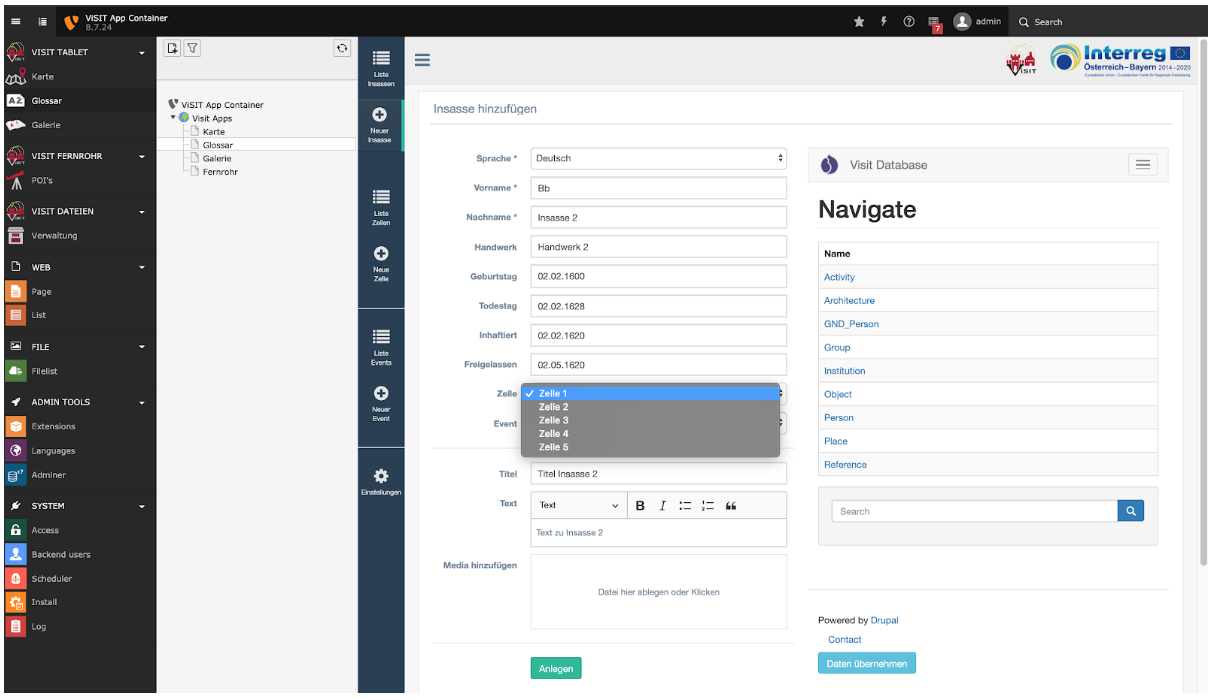
\includegraphics[width=12cm]{Figures/paula/glossar/anlegen_insassen_auswahl.png}
\caption{Anlegen eines Insassens}
\label{img:anlegen_insassen_auswahl}
\end{figure}

Die angelegten Insassen können über \glqq Liste Insassen\grqq{} in der dunkelblauen Leiste angesehen werden (siehe Abbildung \ref{img:angelegte_insassen_listenuebersicht}). Klickt man mittels rechtem Mausklick auf \glqq Glossar\grqq{} im Seitenbaum und wählt \glqq Show\grqq{} aus, kann die Seite im Browser angesehen werden.
\begin{figure}[ht!]
\centering
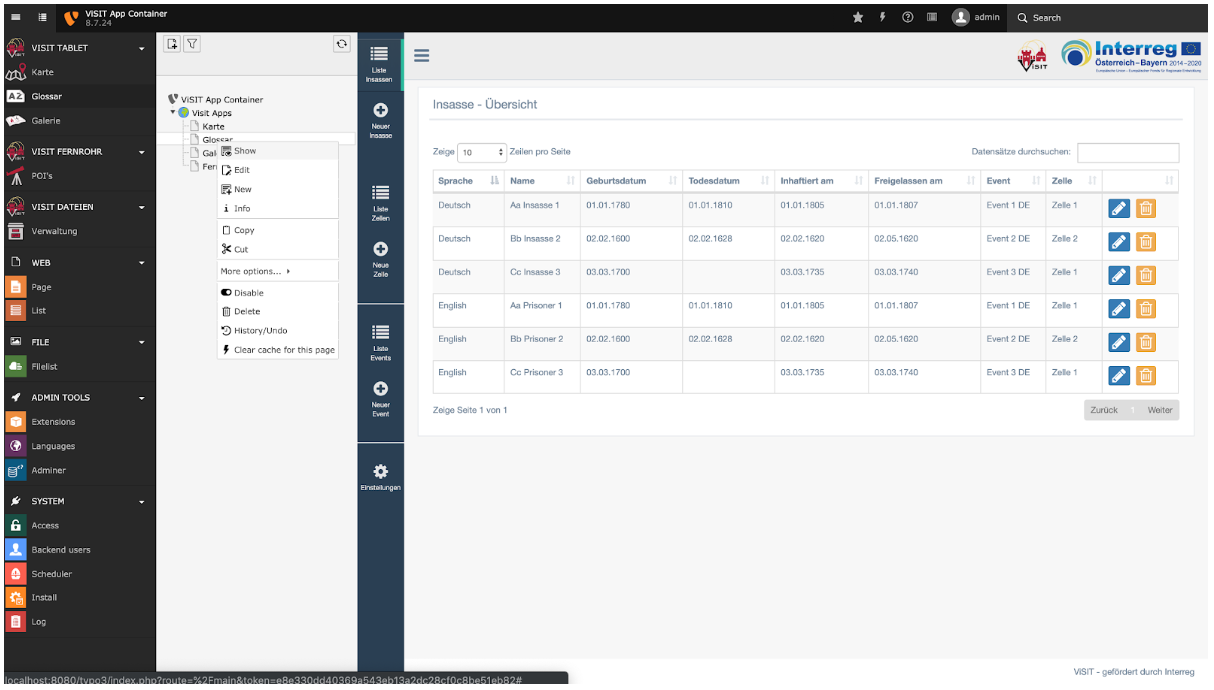
\includegraphics[width=12cm]{Figures/paula/glossar/angelegte_insassen_listenuebersicht.png}
\caption{Angelegte Insassen in der Listenansicht}
\label{img:angelegte_insassen_listenuebersicht}
\end{figure}
Die Insassen werden im Browser, nach dem Auswählen der bevorzugten Sprache, angezeigt.
\begin{figure}[ht!]
\centering
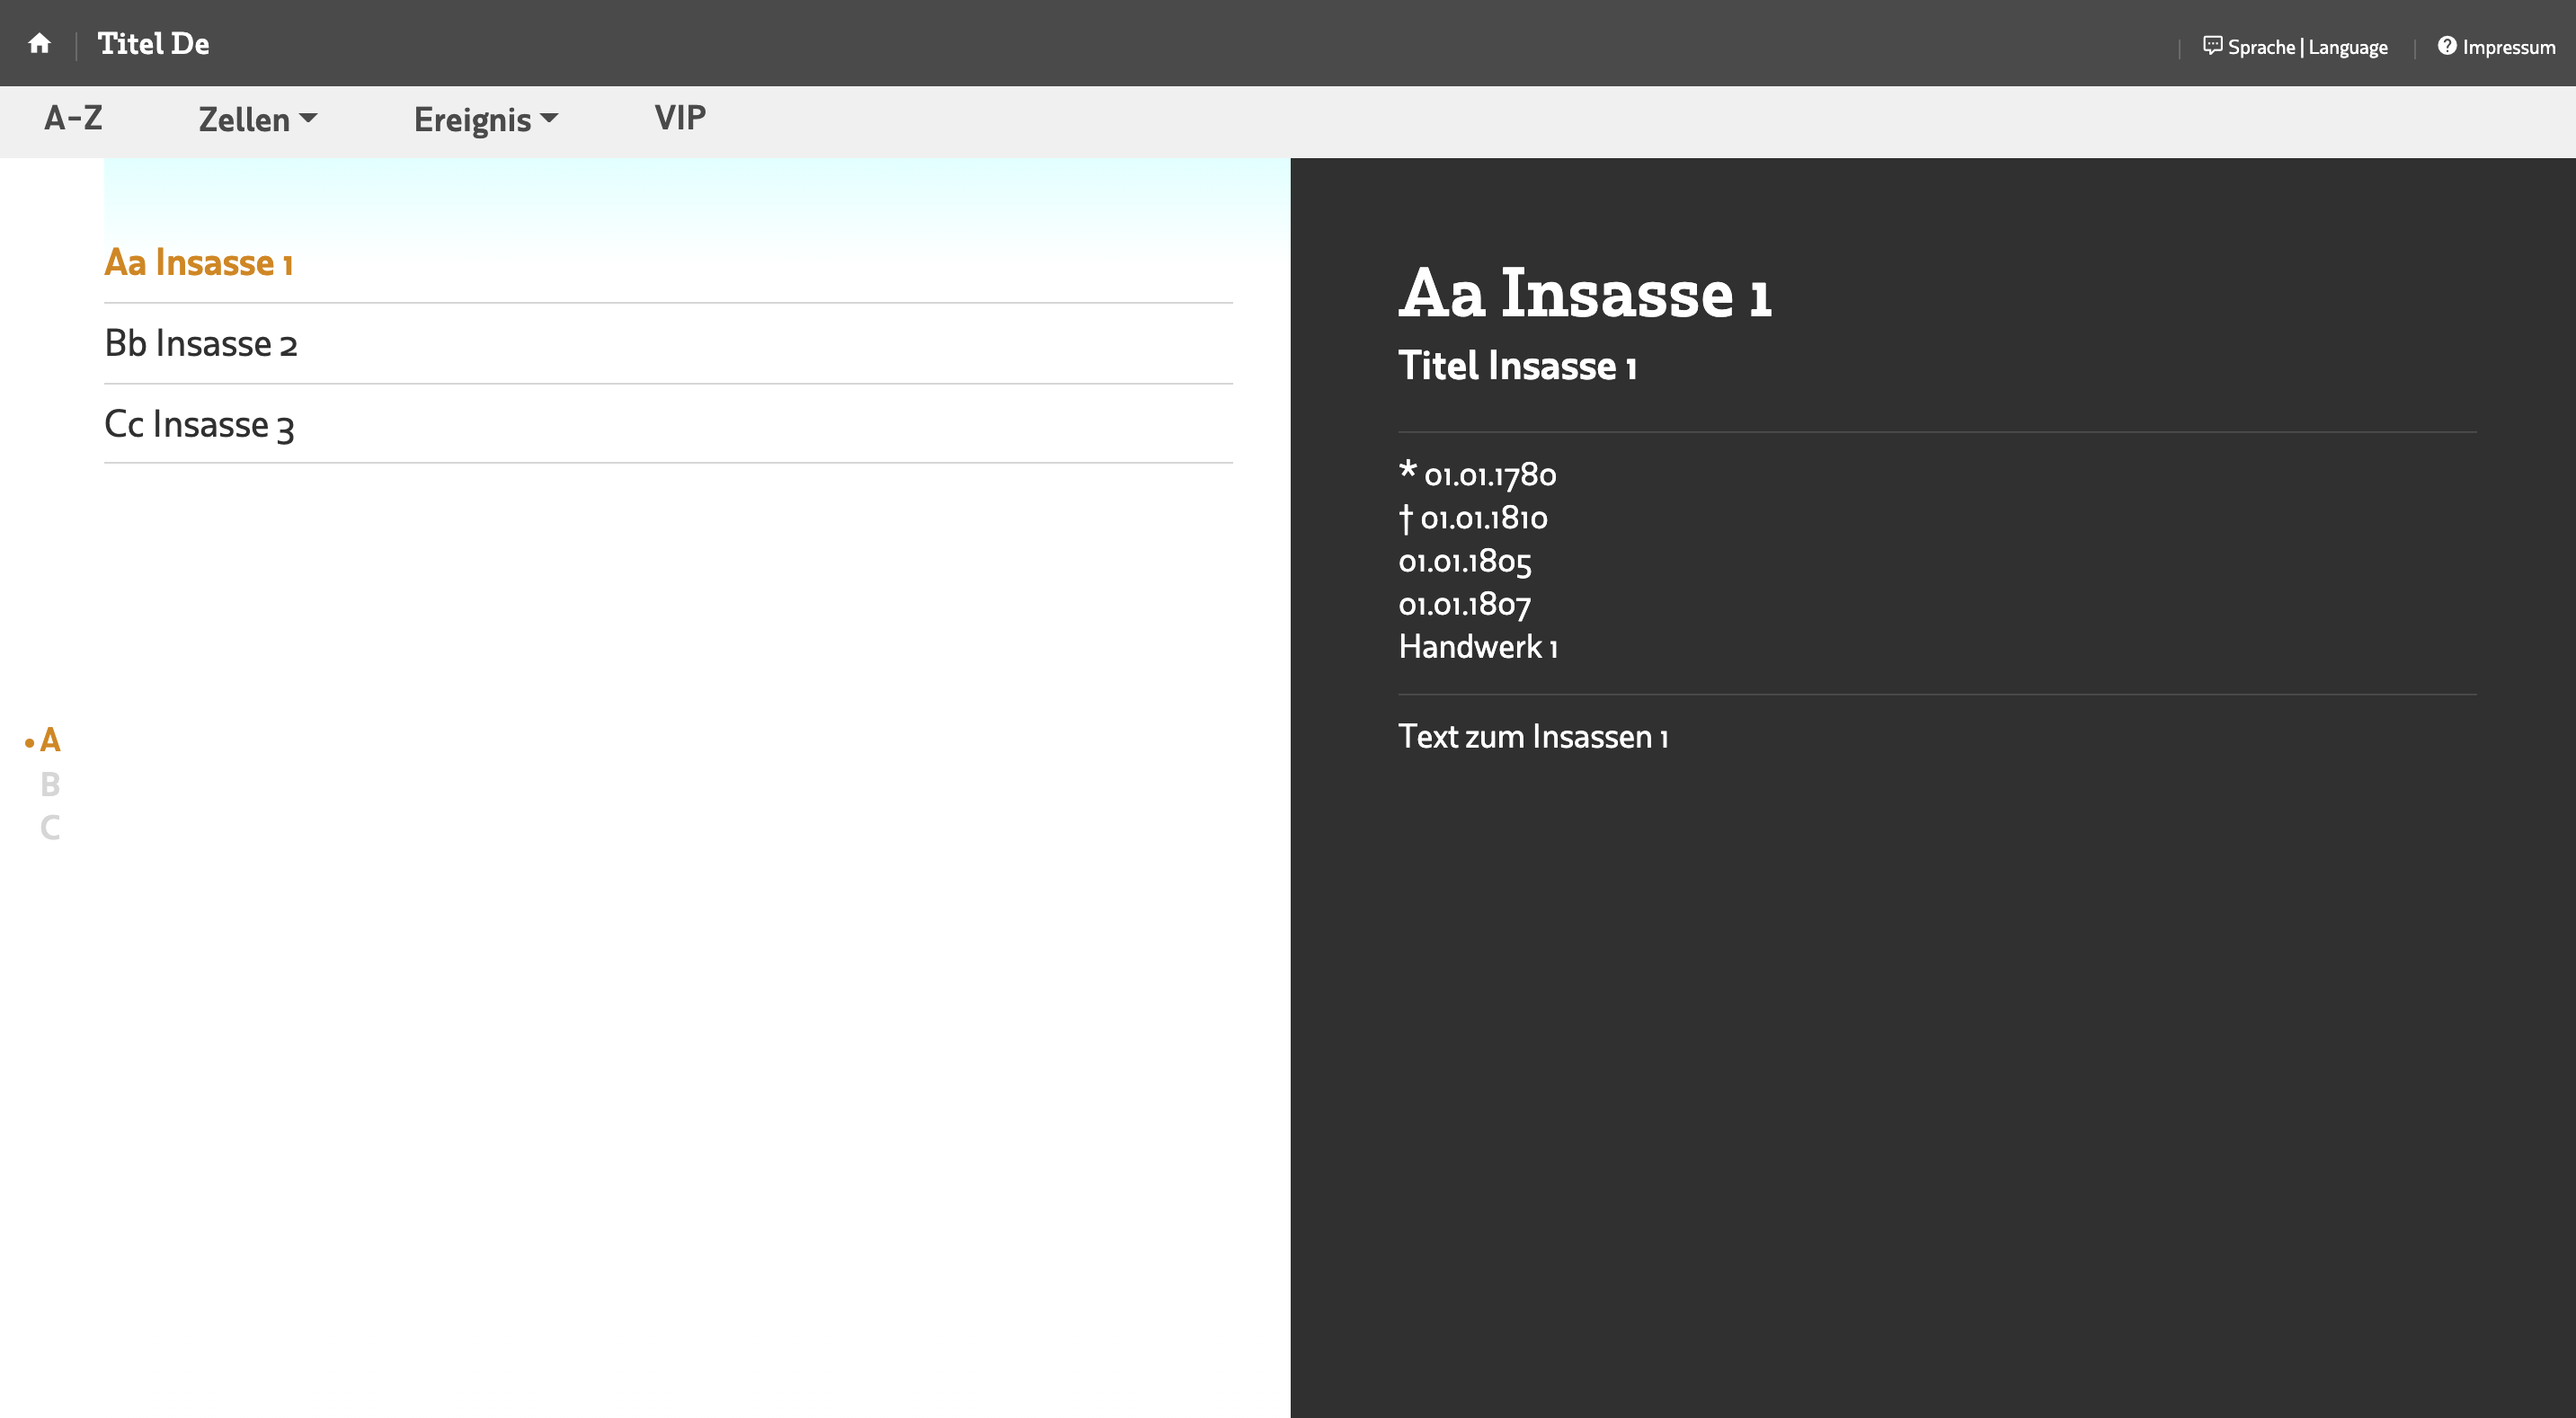
\includegraphics[width=12cm]{Figures/paula/glossar/insassenuebersicht_browser.png}
\caption{Ansicht der Insassen im Browser}
\label{img:insassenuebersicht_browser}
\end{figure}

\subsection{Bearbeitung und Löschung von Insassen, Events und Zellen}

Insassen, Zellen und Events können jederzeit einzeln bearbeitet oder gelöscht werden. Dies geht, indem zuerst die jeweilige Listenansicht (Liste Insassen/Zellen/Events) in der dunkelblauen Leiste ausgewählt wird. In weiterer Folge kann jedes einzelne Element (Zeile) aus der Liste einzeln bearbeitet oder gelöscht werden. Zum Bearbeiten auf das blaue Stiftsymbol auf der rechten Seite der gewünschten Zeile klicken, zum Löschen des Objekts, den orangen Müllkübel (siehe Abbildung \ref{img:loeschung_insassen}).

\begin{figure}[ht!]
\centering
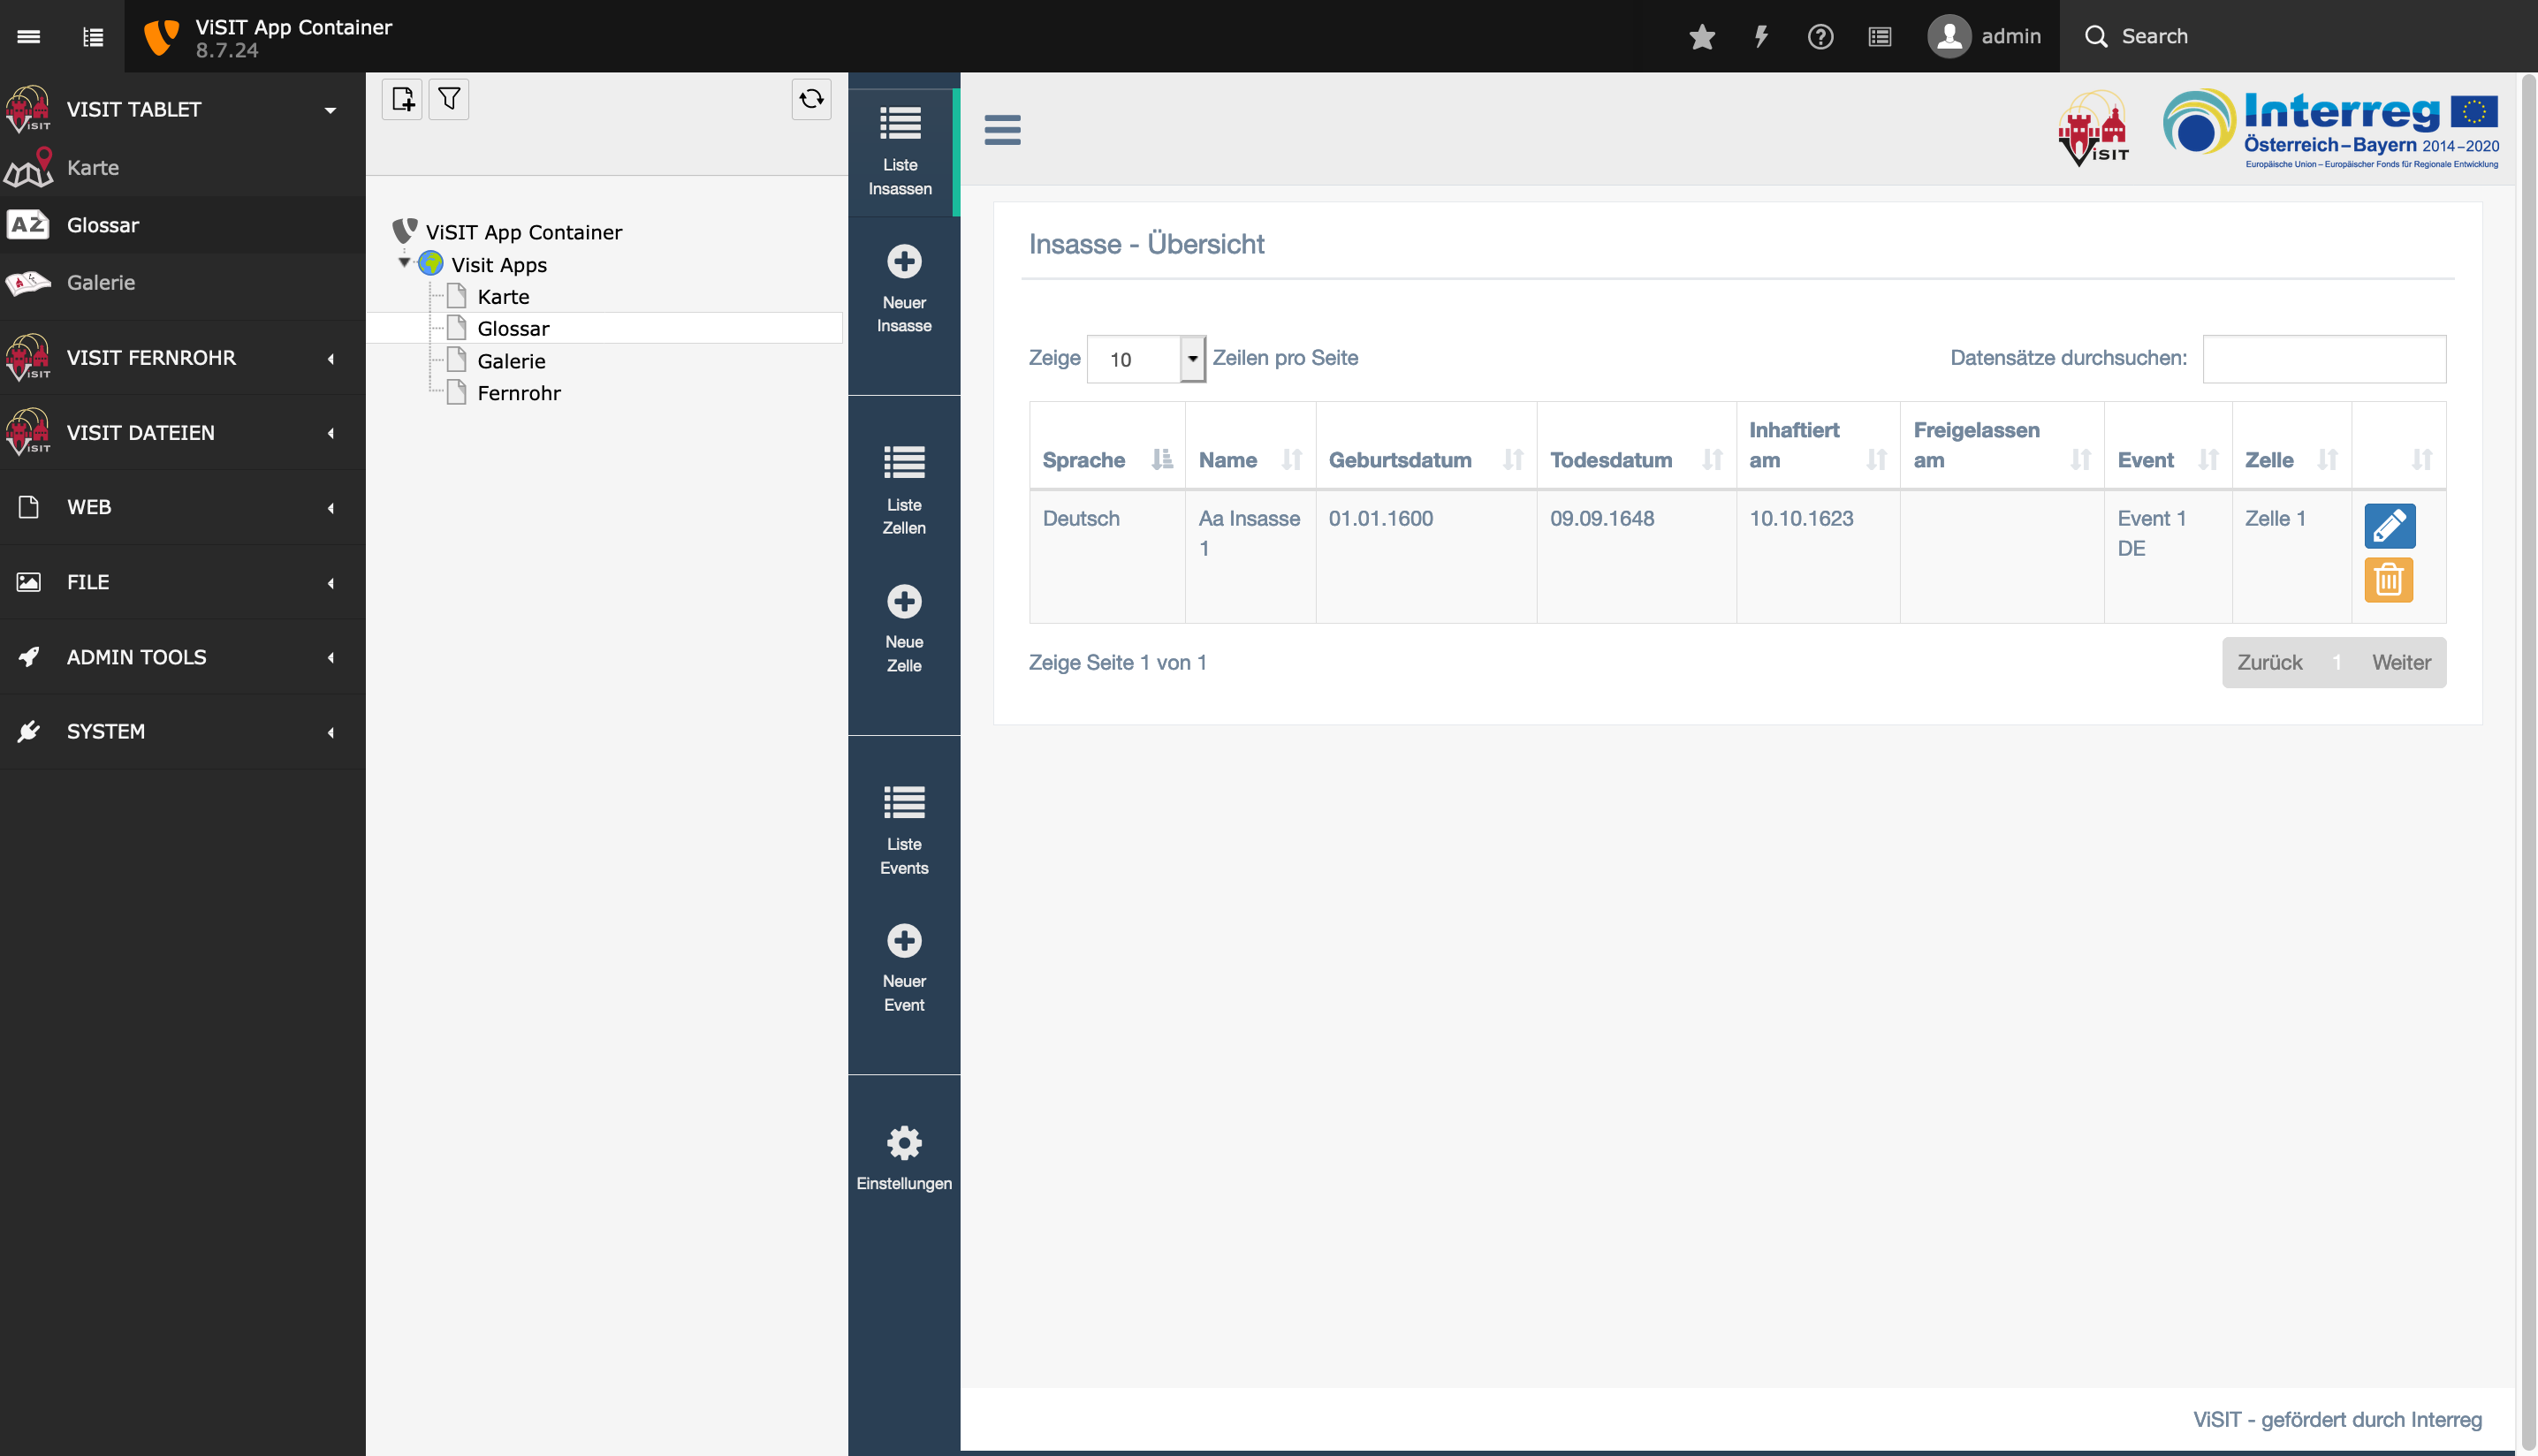
\includegraphics[width=12cm]{Figures/paula/glossar/loeschen_bearbeiten_insasse.png}
\caption{Bearbeitung bzw. Löschung von Insassen/Zellen/Events}
\label{img:loeschung_insassen}
\end{figure}


\cleardoublepage

\section{Galerie-Applikation}

In der Galerie-Applikation kann der Benutzer aus verschiedenen Teasern auswählen, wird ein Teaser ausgewählt gelangt der Besucher zu den Inhaltselementen und kann diese lesen. Die Inhaltselemente wiederum können aus mehreren Subelementen bestehen. Der Benutzer muss hinunter scrollen beziehungsweise swipen.
Wird nach rechts oder links geswiped, dann wird entweder das vorhergehende oder das nachkommende Inhaltselement (mit den dazugehörigen Subelementen) angezeigt.
Nach einer bestimmten Zeit ohne einer Interaktion kehrt die Applikation zum Menü zurück und zeigt den Startbildschirm an.

\subsection{Einpflegen der Daten in die Galerie-Applikation}

Dazu aus der Modulleiste links unter der Obergruppe VISIT TABLET die Karte auswählen. Im linken Teil des Hauptfensters ist der Seitenbaum zu sehen und rechts befindet sich die Kartenübersicht. Oben links im rechten Teil des Hauptfensters befindet sich ein Menü-Button, wird dieser angeklickt, wird eine weitere dunkelblaue Spalte zwischen dem Seitenbaum und dem Arbeitsbereich im Hauptfenster sichtbar (siehe Abbildung \ref{img:uebersicht_galerie}).

\begin{figure}[ht!]
\centering
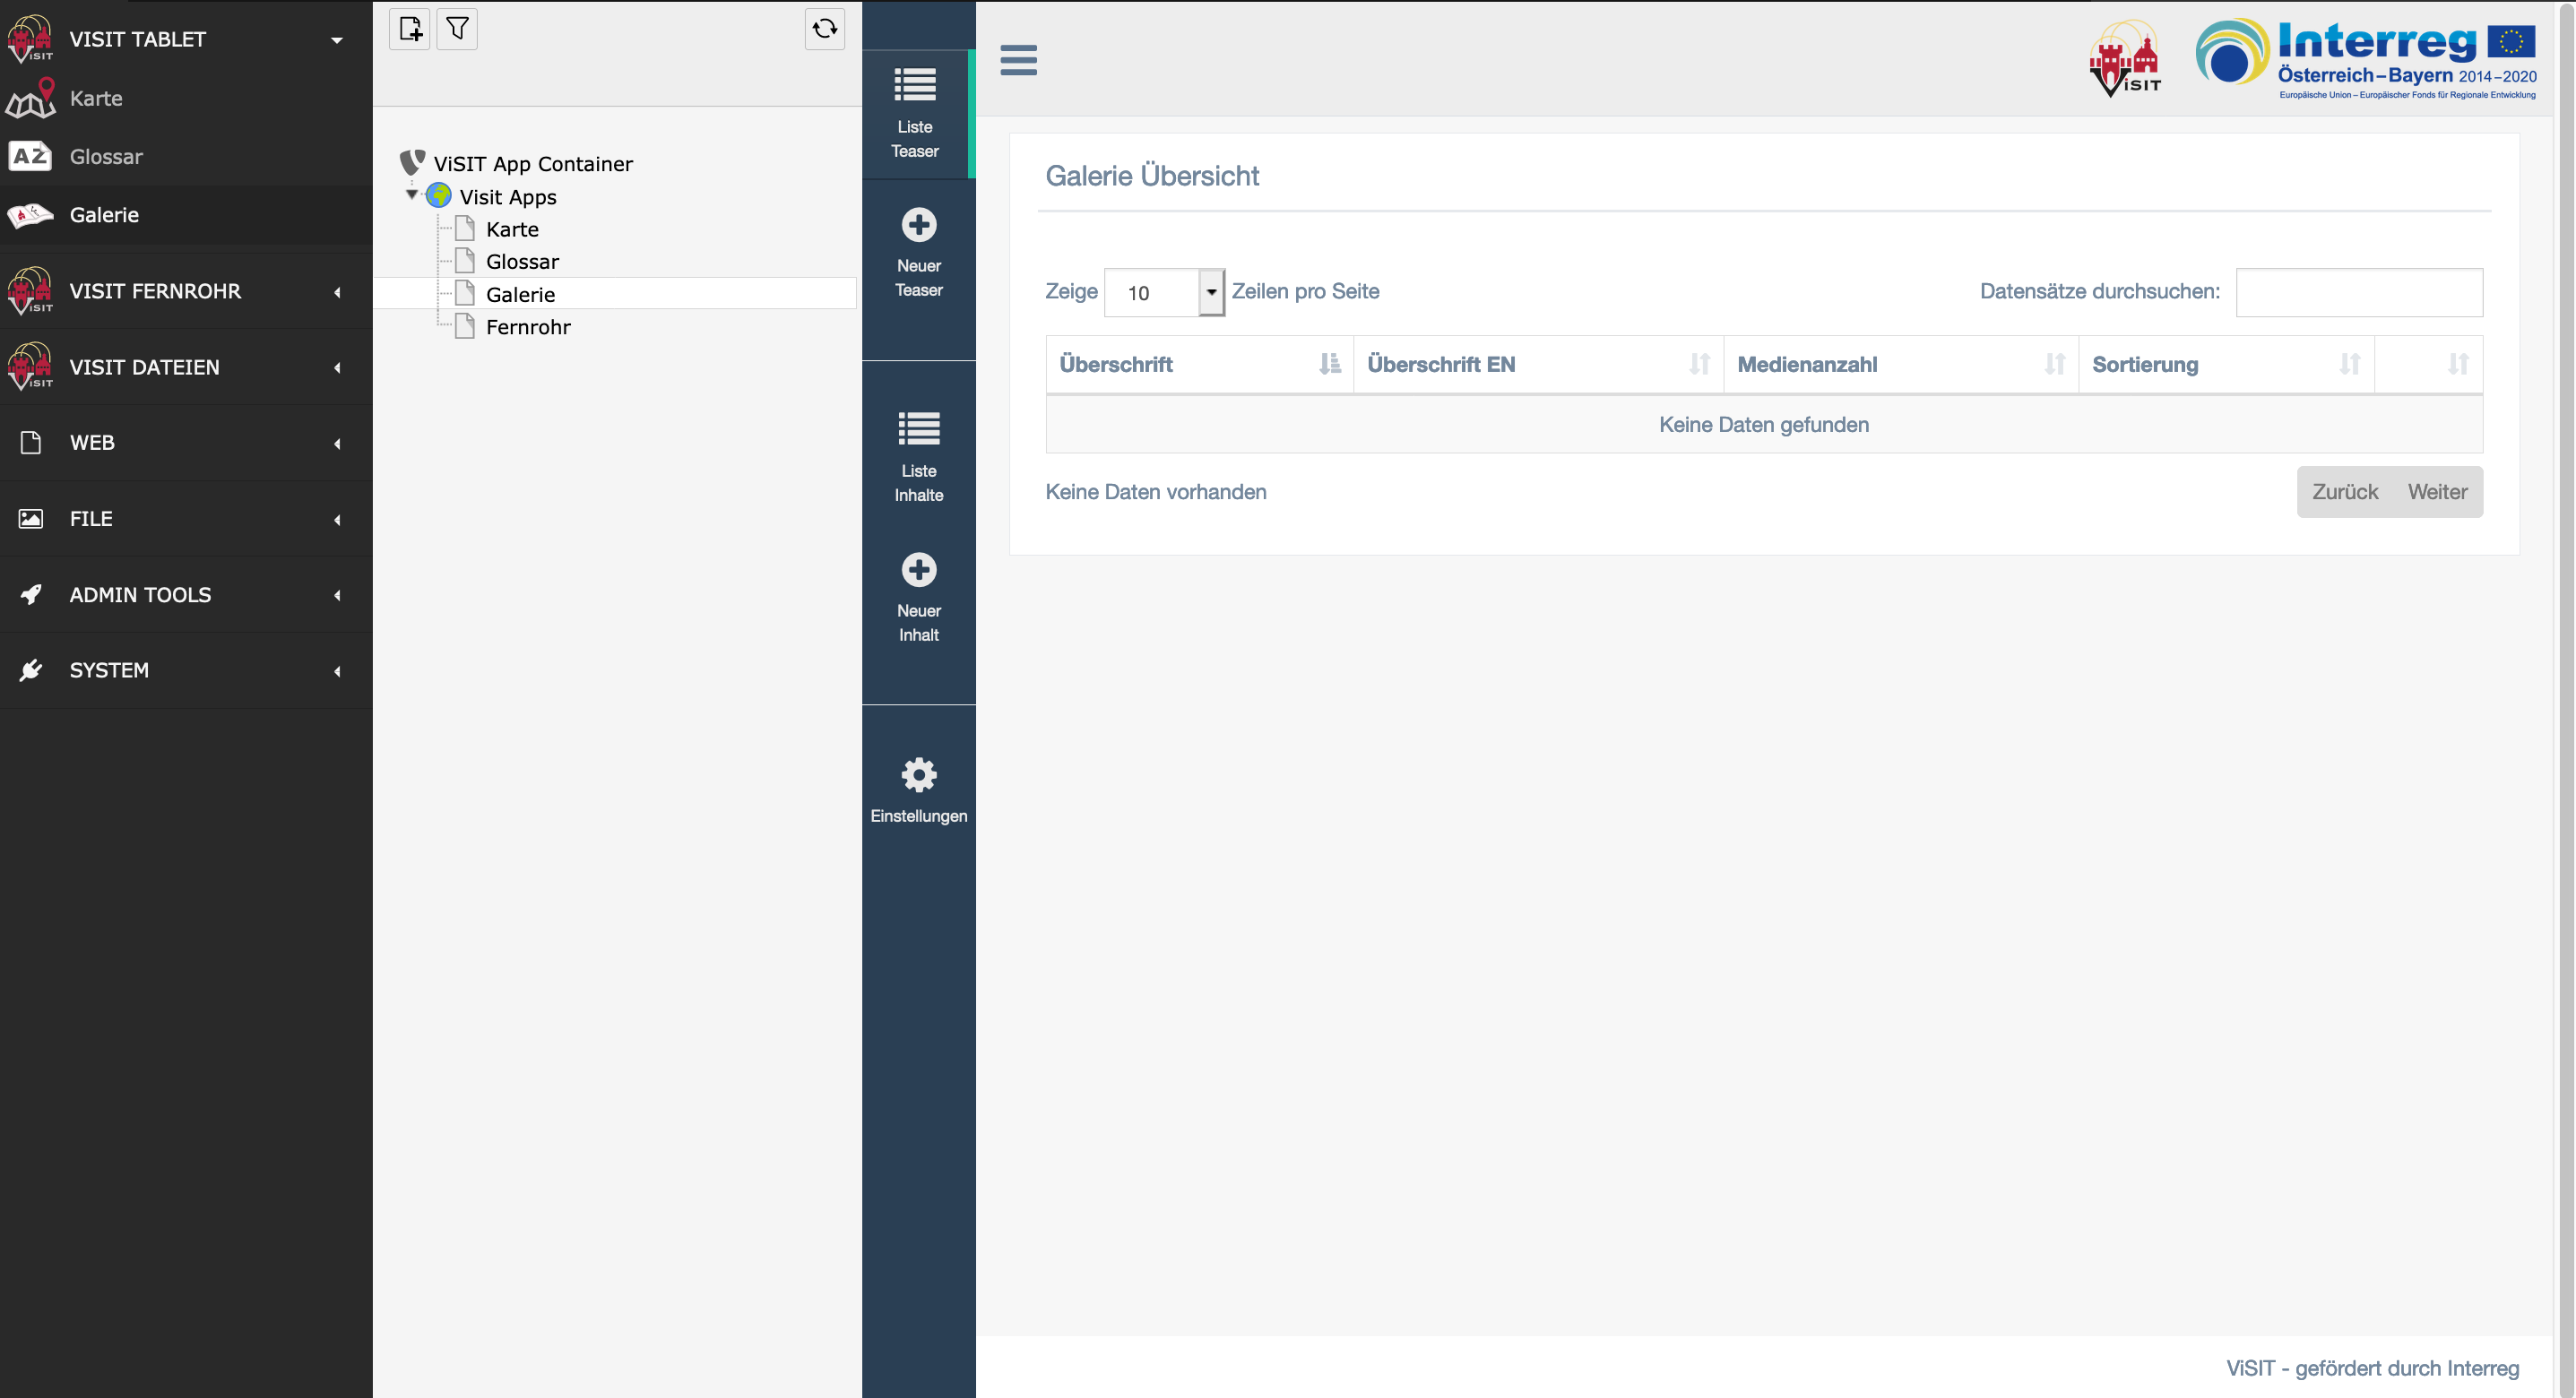
\includegraphics[width=12cm]{Figures/paula/galerie/uebersicht_galerie.png}
\caption{Übersicht über alle erstellten Inhalte}
\label{img:uebersicht_galerie}
\end{figure}

\subsection{Auswahl des gewünschten Layouts für die Startseite}

Dazu in der dunkelblauen Leiste \glqq Einstellungen\grqq{} auswählen (siehe Abbildung  \ref{img:auswahl_layout}). Zur Auswahl gibt es hier entweder das 3er-Layout mit 3 Spalten und 1 Zeile (siehe Abbildung \ref{img:layout_3er}) oder das 6er-Layout mit 3 Spalten und 2 Zeilen (siehe Abbildung \ref{img:layout_6er}) für die Teaser auf der Startseite.

\begin{figure}[ht!]
\centering
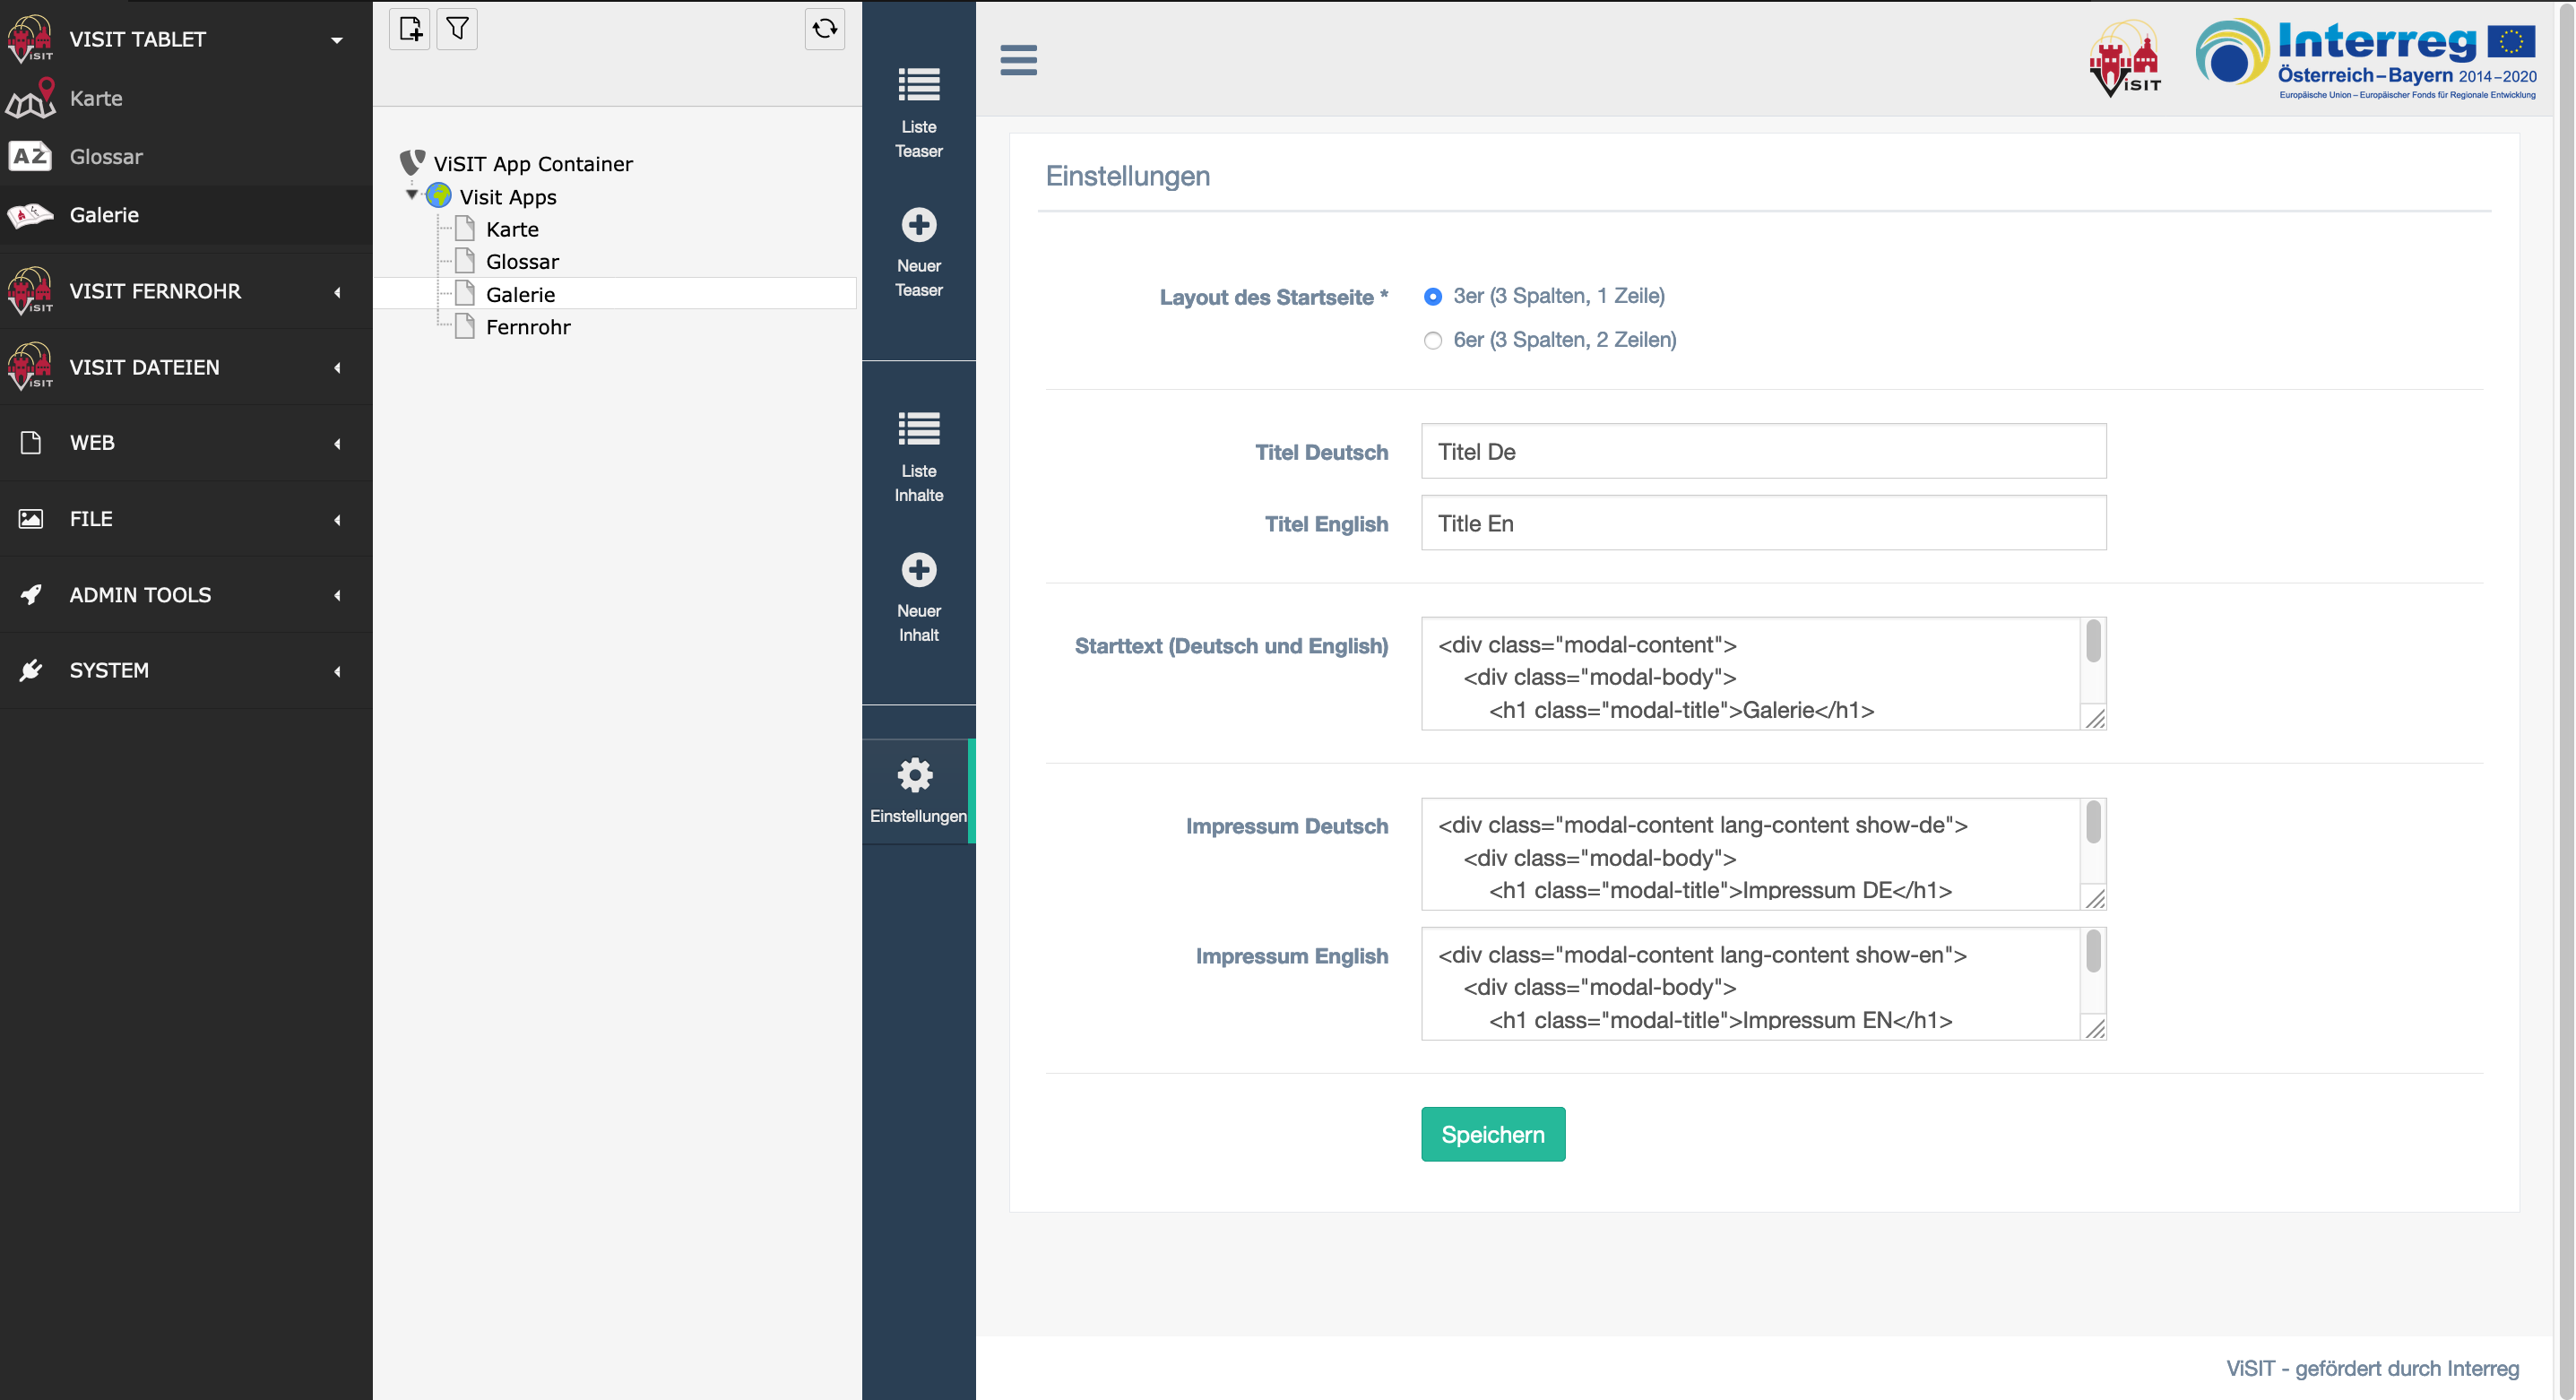
\includegraphics[width=12cm]{Figures/paula/galerie/auswahl_layout.png}
\caption{Auswahl des gewünschten Layouts in den Einstellungen}
\label{img:auswahl_layout}
\end{figure}

\begin{figure}[ht!]
\centering
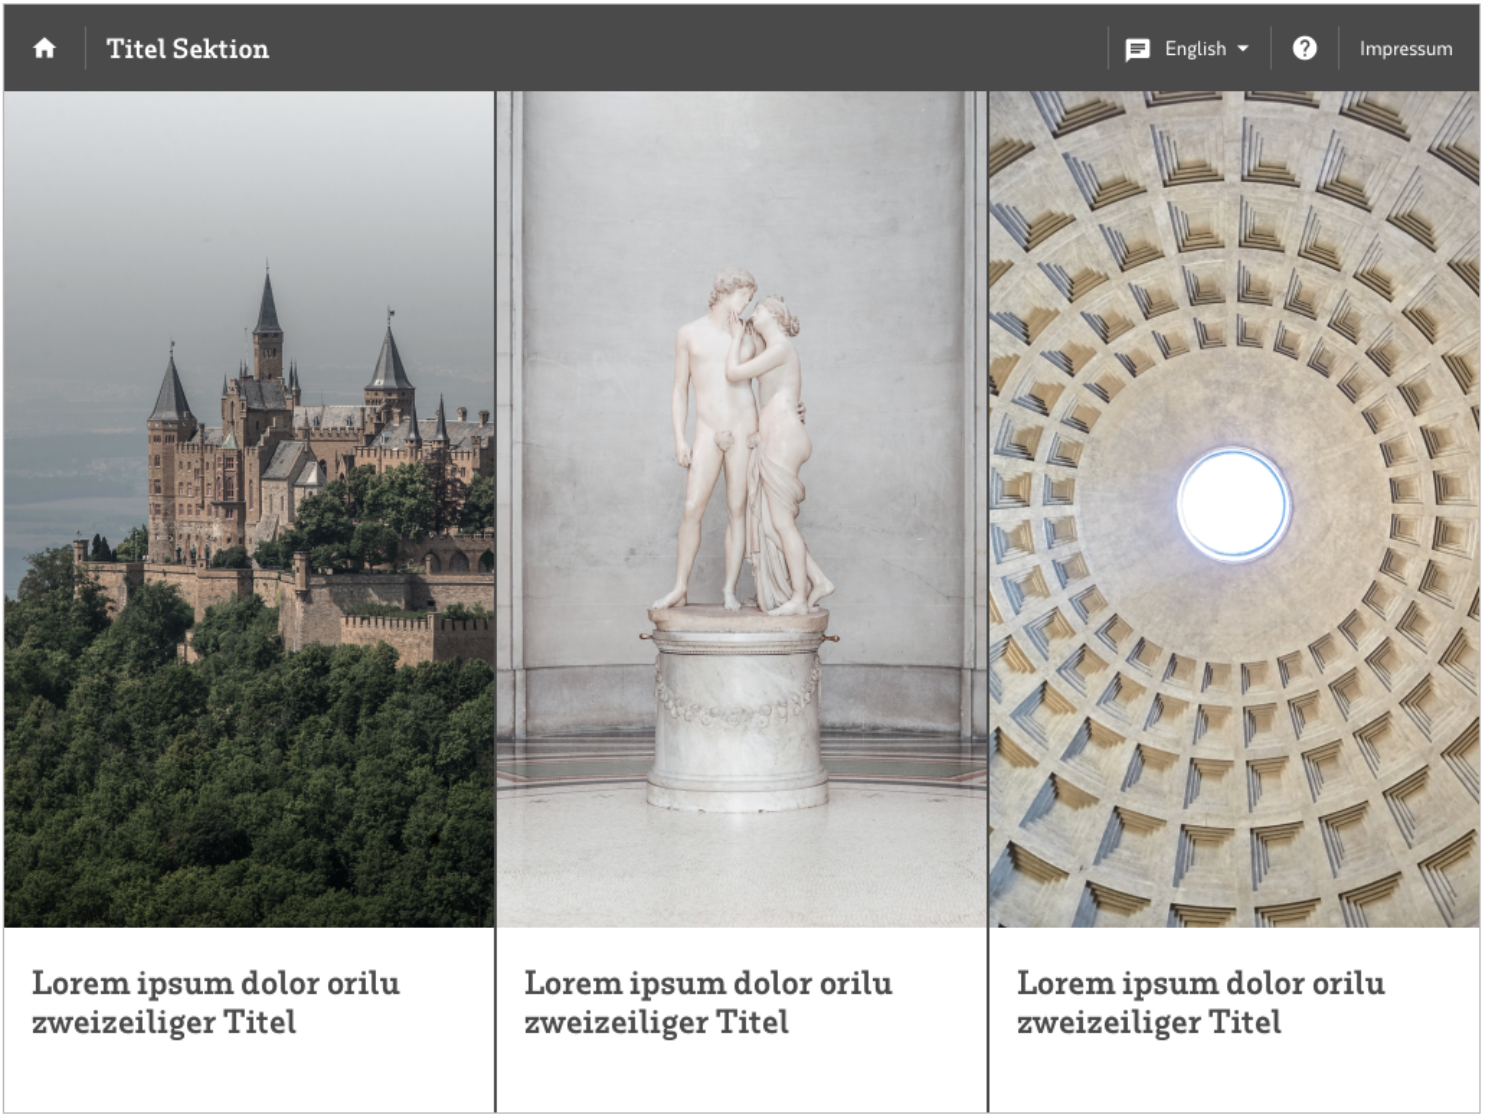
\includegraphics[width=12cm]{Figures/paula/galerie/layout_3er.png}
\caption{3er-Layout (3 Spalten, 1 Zeile)}
\label{img:layout_3er}
\end{figure}

\begin{figure}[ht!]
\centering
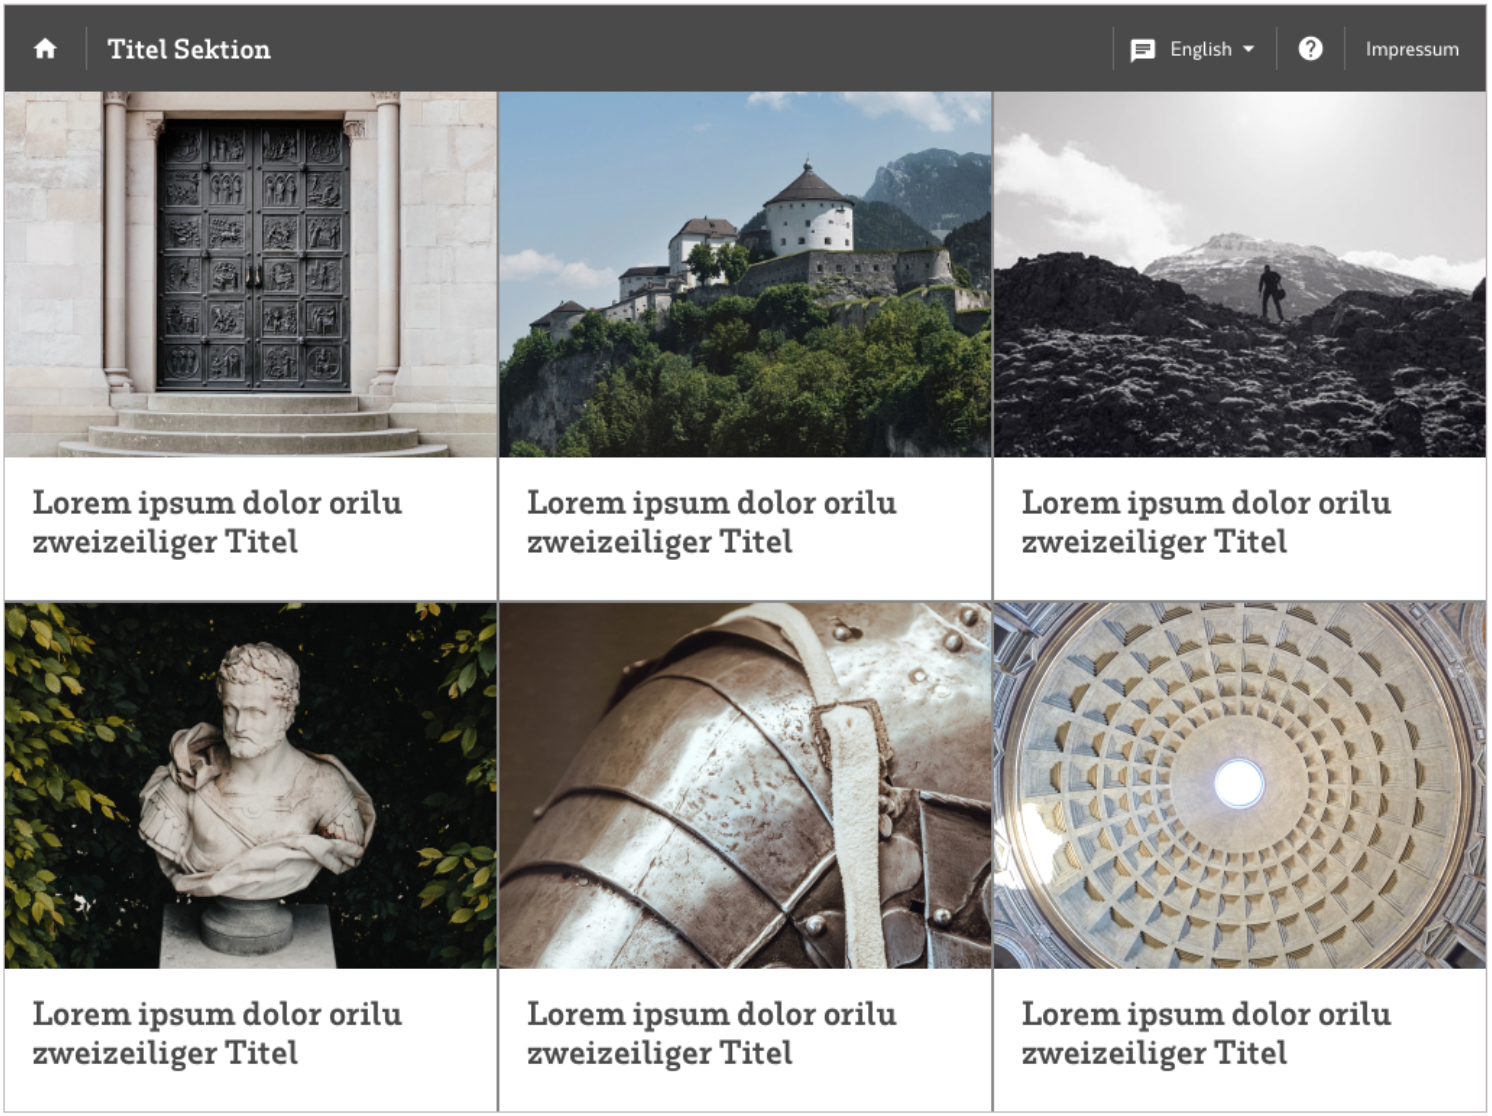
\includegraphics[width=12cm]{Figures/paula/galerie/layout_6er.png}
\caption{6er-Layout (3 Spalten, 2 Zeilen)}
\label{img:layout_6er}
\end{figure}


\subsection{Erstellung der Startseite für die Galerie-Applikation}

Die Galerie kann mit einem Klick auf \glqq Galerie\grqq{} in der Modulleiste konfiguriert werden (siehe Abbildung \ref{img:auswahl_layout}).


Die Startseite der Applikation kann unter \glqq Einstellungen\grqq{} in der dunkelblauen Leiste konfiguriert werden. Dafür benötigt man den Text für die Startseite \url{https://github.com/ViSIT-Dev/appbundle}. Dieser Text muss in die entsprechenden Inputfelder kopiert werden (siehe Abbildung \ref{img:auswahl_layout}).


Nachdem die Startseite befüllt wurde, wird sie dem Besucher als erstes angezeigt, auf dieser kann der Besucher dann die gewünschte Sprache auswählen (siehe Abbildung \ref{img:startseite}).

\begin{figure}[ht!]
\centering
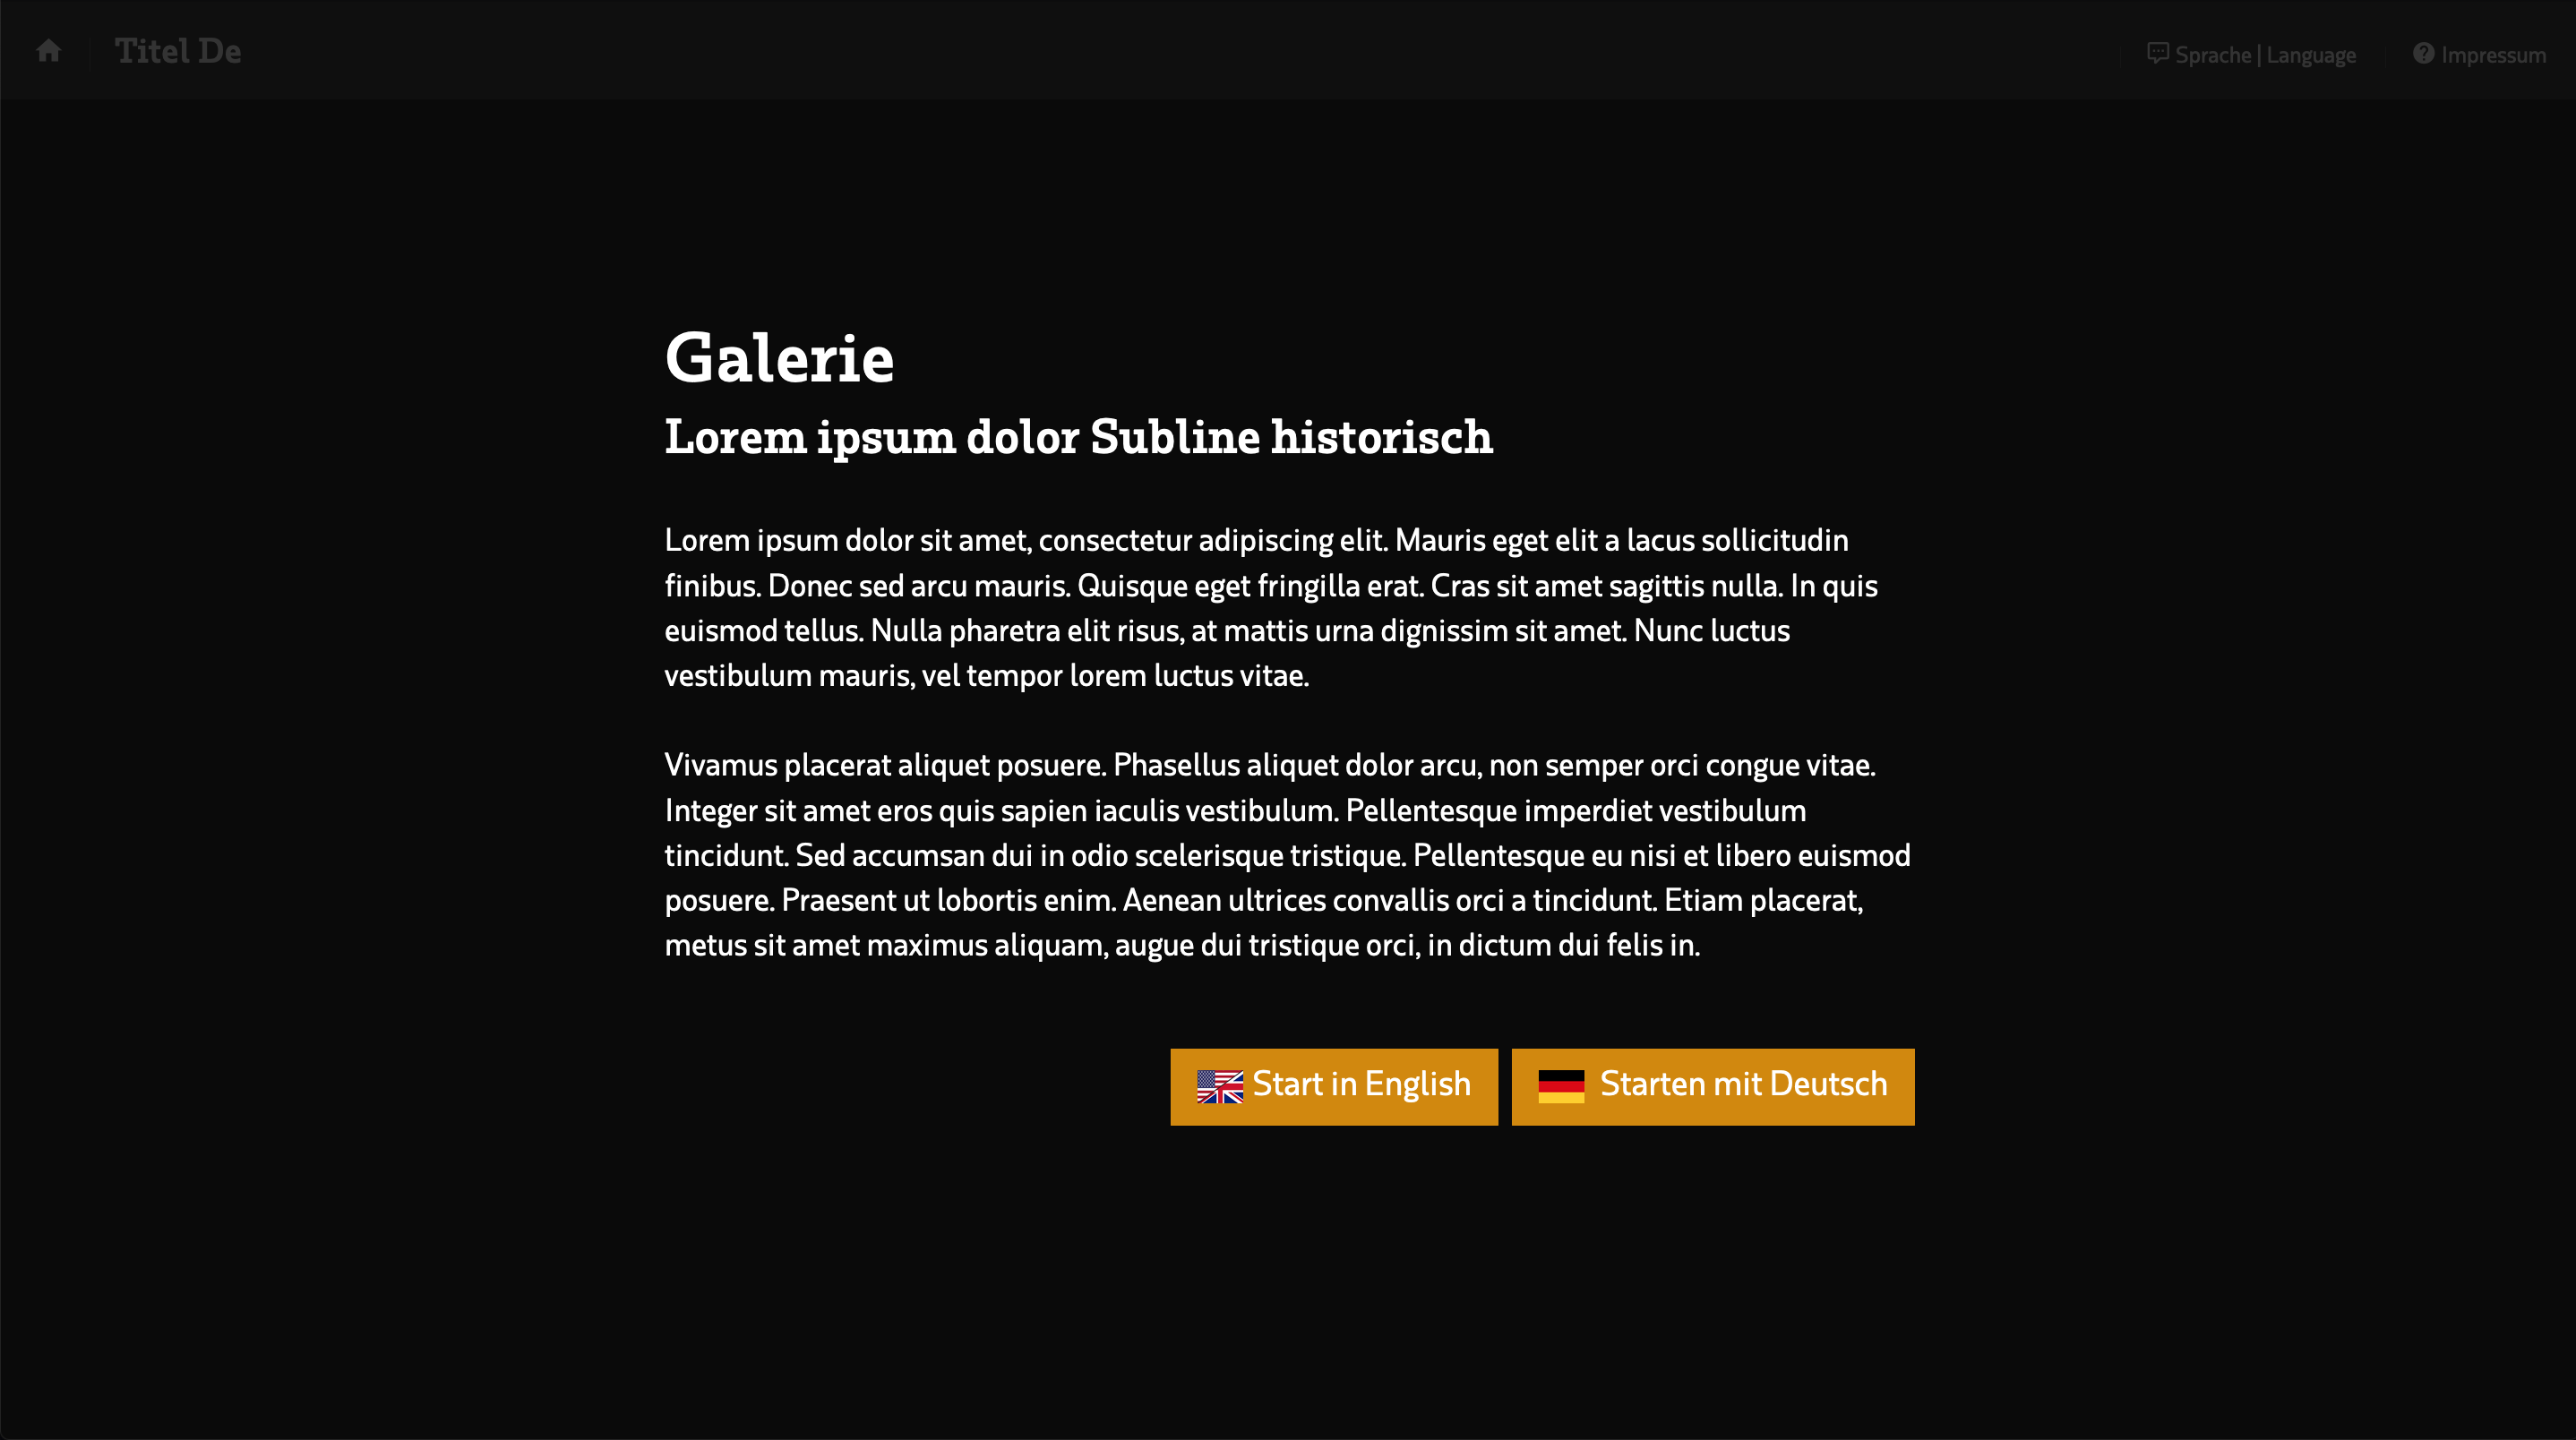
\includegraphics[width=12cm]{Figures/paula/galerie/startseite.png}
\caption{Startseite der Galerie-Applikation}
\label{img:startseite}
\end{figure}



\subsection{Neues Inhaltselement anlegen}

Als erstes muss ein neues Inhaltselement angelegt werden. Dies geschieht über einen Klick auf \glqq Neuer Inhalt\grqq{} in der dunkelblauen Leiste (siehe Abbildung \ref{img:neues_inhaltselement_anlegen}).

\begin{figure}[ht!]
\centering
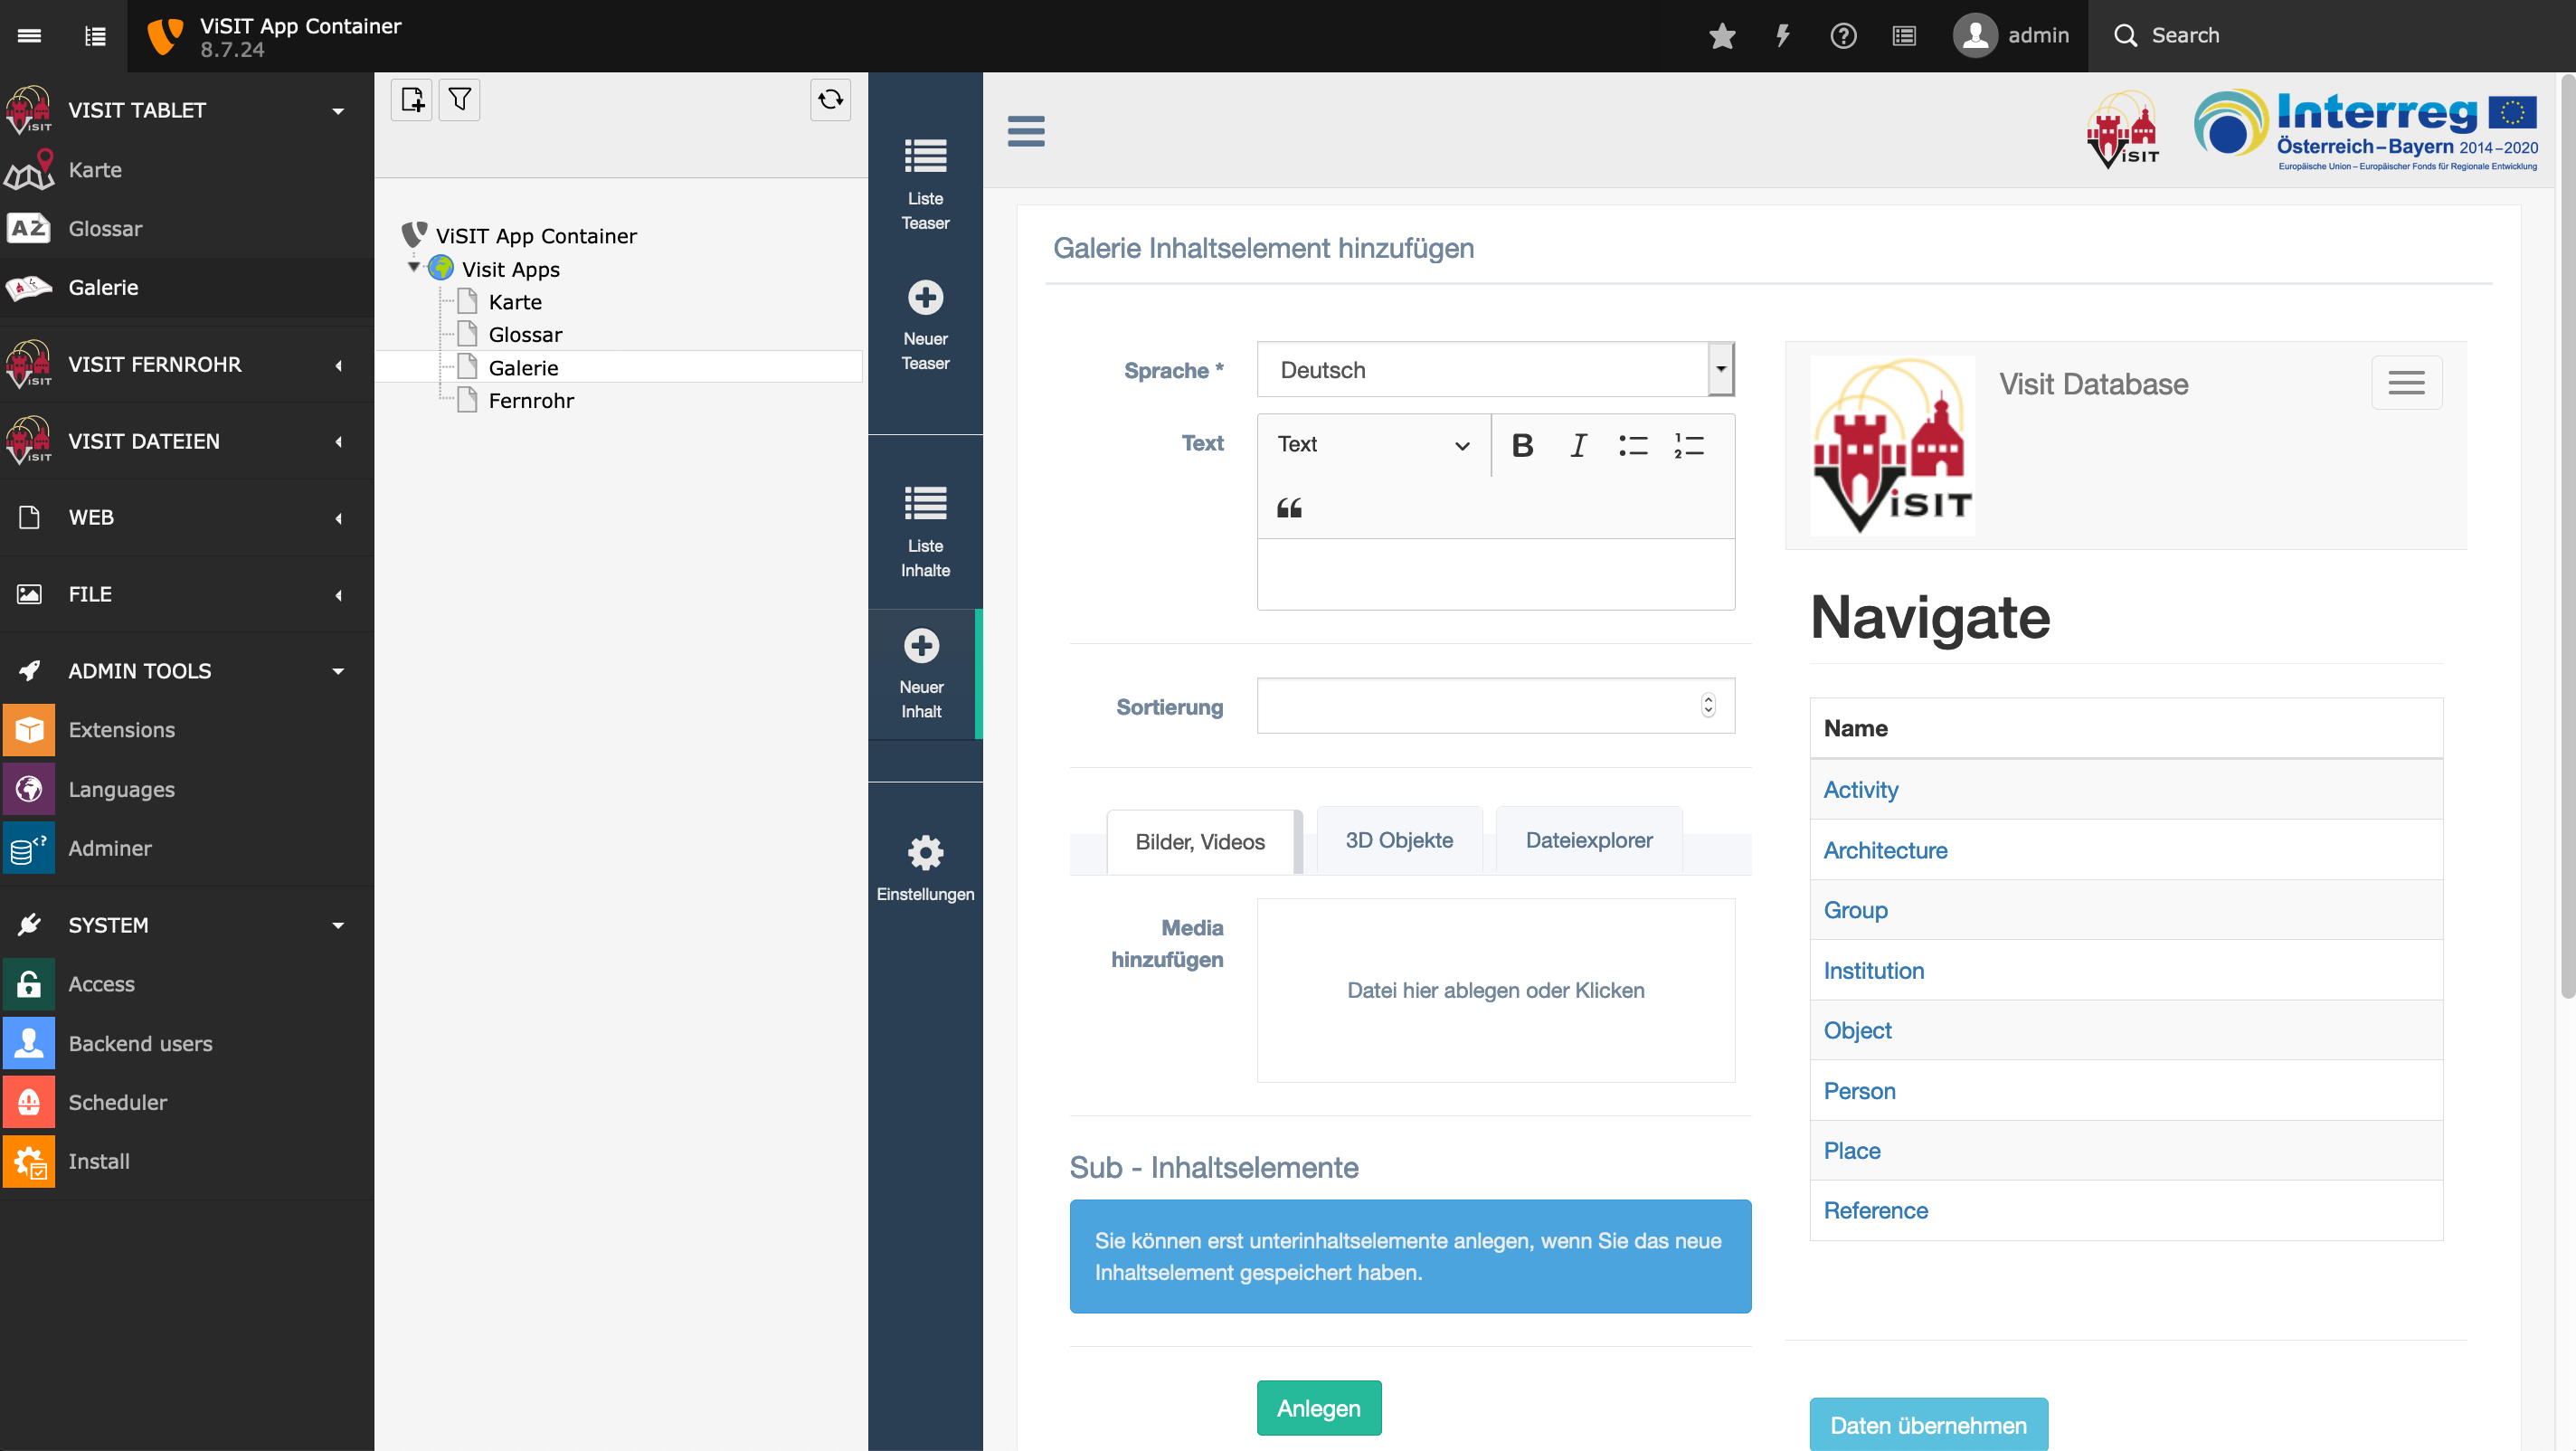
\includegraphics[width=12cm]{Figures/paula/galerie/neues_inhaltselement_anlegen.png}
\caption{Neues Inhaltselement anlegen}
\label{img:neues_inhaltselement_anlegen}
\end{figure}

Im nächsten Schritt muss zuerst die Sprache ausgewählt werden. Dann wird das Textfeld befüllt und ein Medienobjekt kann zugefügt werden. Bei diesem Text und Medienobjekt handelt es sich um den obersten Text (siehe Abbildung \ref{img:ansicht_inhaltselement_galerie} blau eingerahmter Bereich).

\begin{figure}[ht!]
\centering
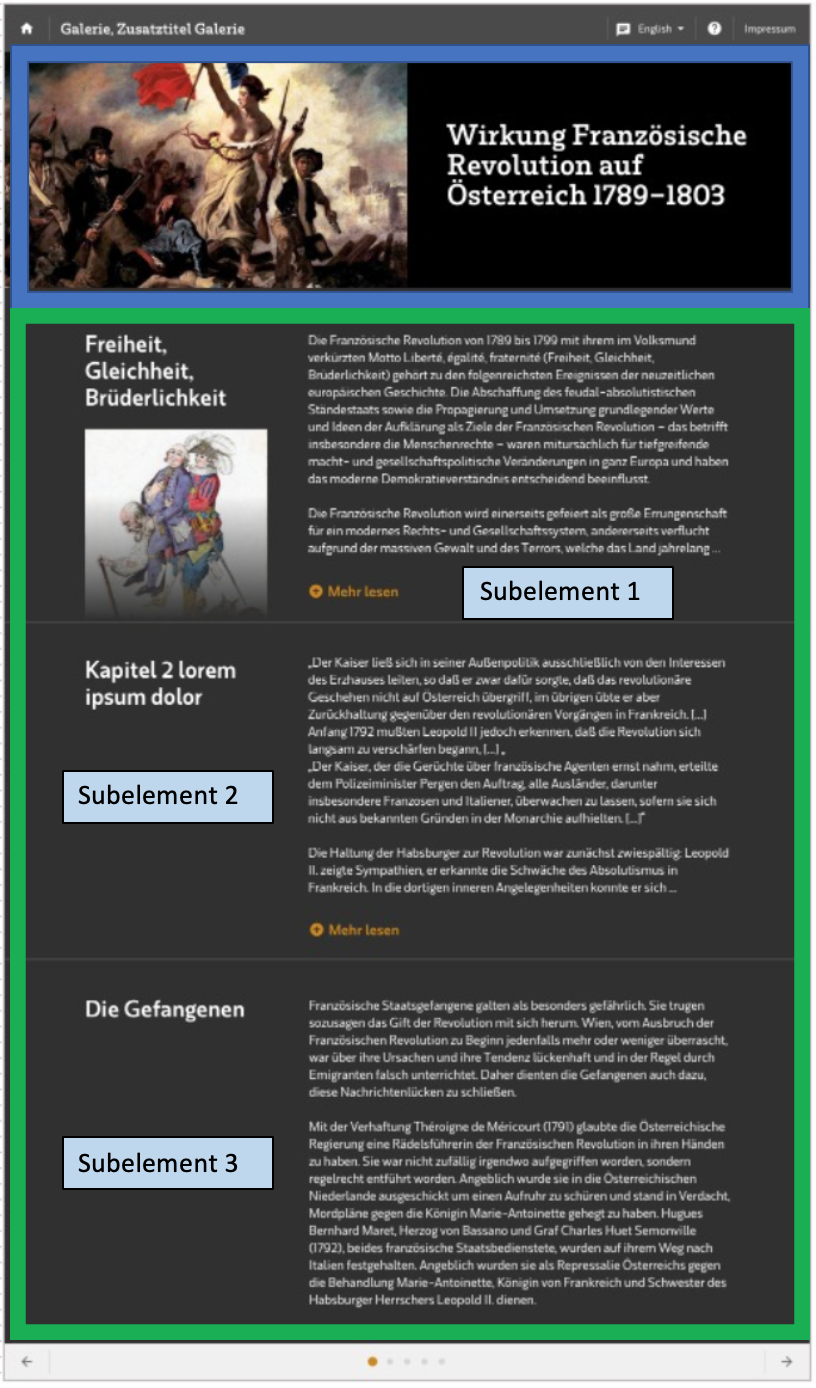
\includegraphics[width=12cm]{Figures/paula/galerie/ansicht_inhaltselement_galerie.png}
\caption{Ansicht eines Inhaltselements aus der Galerie auf einem Tablet}
\label{img:ansicht_inhaltselement_galerie}
\end{figure}

\subsection{Sortierung der Inhaltselemente}

Die Sortierung der Inhaltselemente gibt an, in welcher Reihenfolge die einzelnen Inhaltselemente durchgeswiped (sowohl nach rechts als auch nach links) werden können.


\subsection{Anlegen eines Sub-Inhaltselements}
Nachdem das Inhaltselement angelegt und gespeichert wurde, können - müssen aber nicht - weitere Sub-Inhaltselemente hinzugefügt werden (siehe Abbildung \ref{img:anlegen_neuer_Sub_inhaltselemente} sowie Abbildung \ref{img:ansicht_inhaltselement_galerie} grün eingerahmte Sub-Inhaltselemente).

\begin{figure}[ht!]
\centering
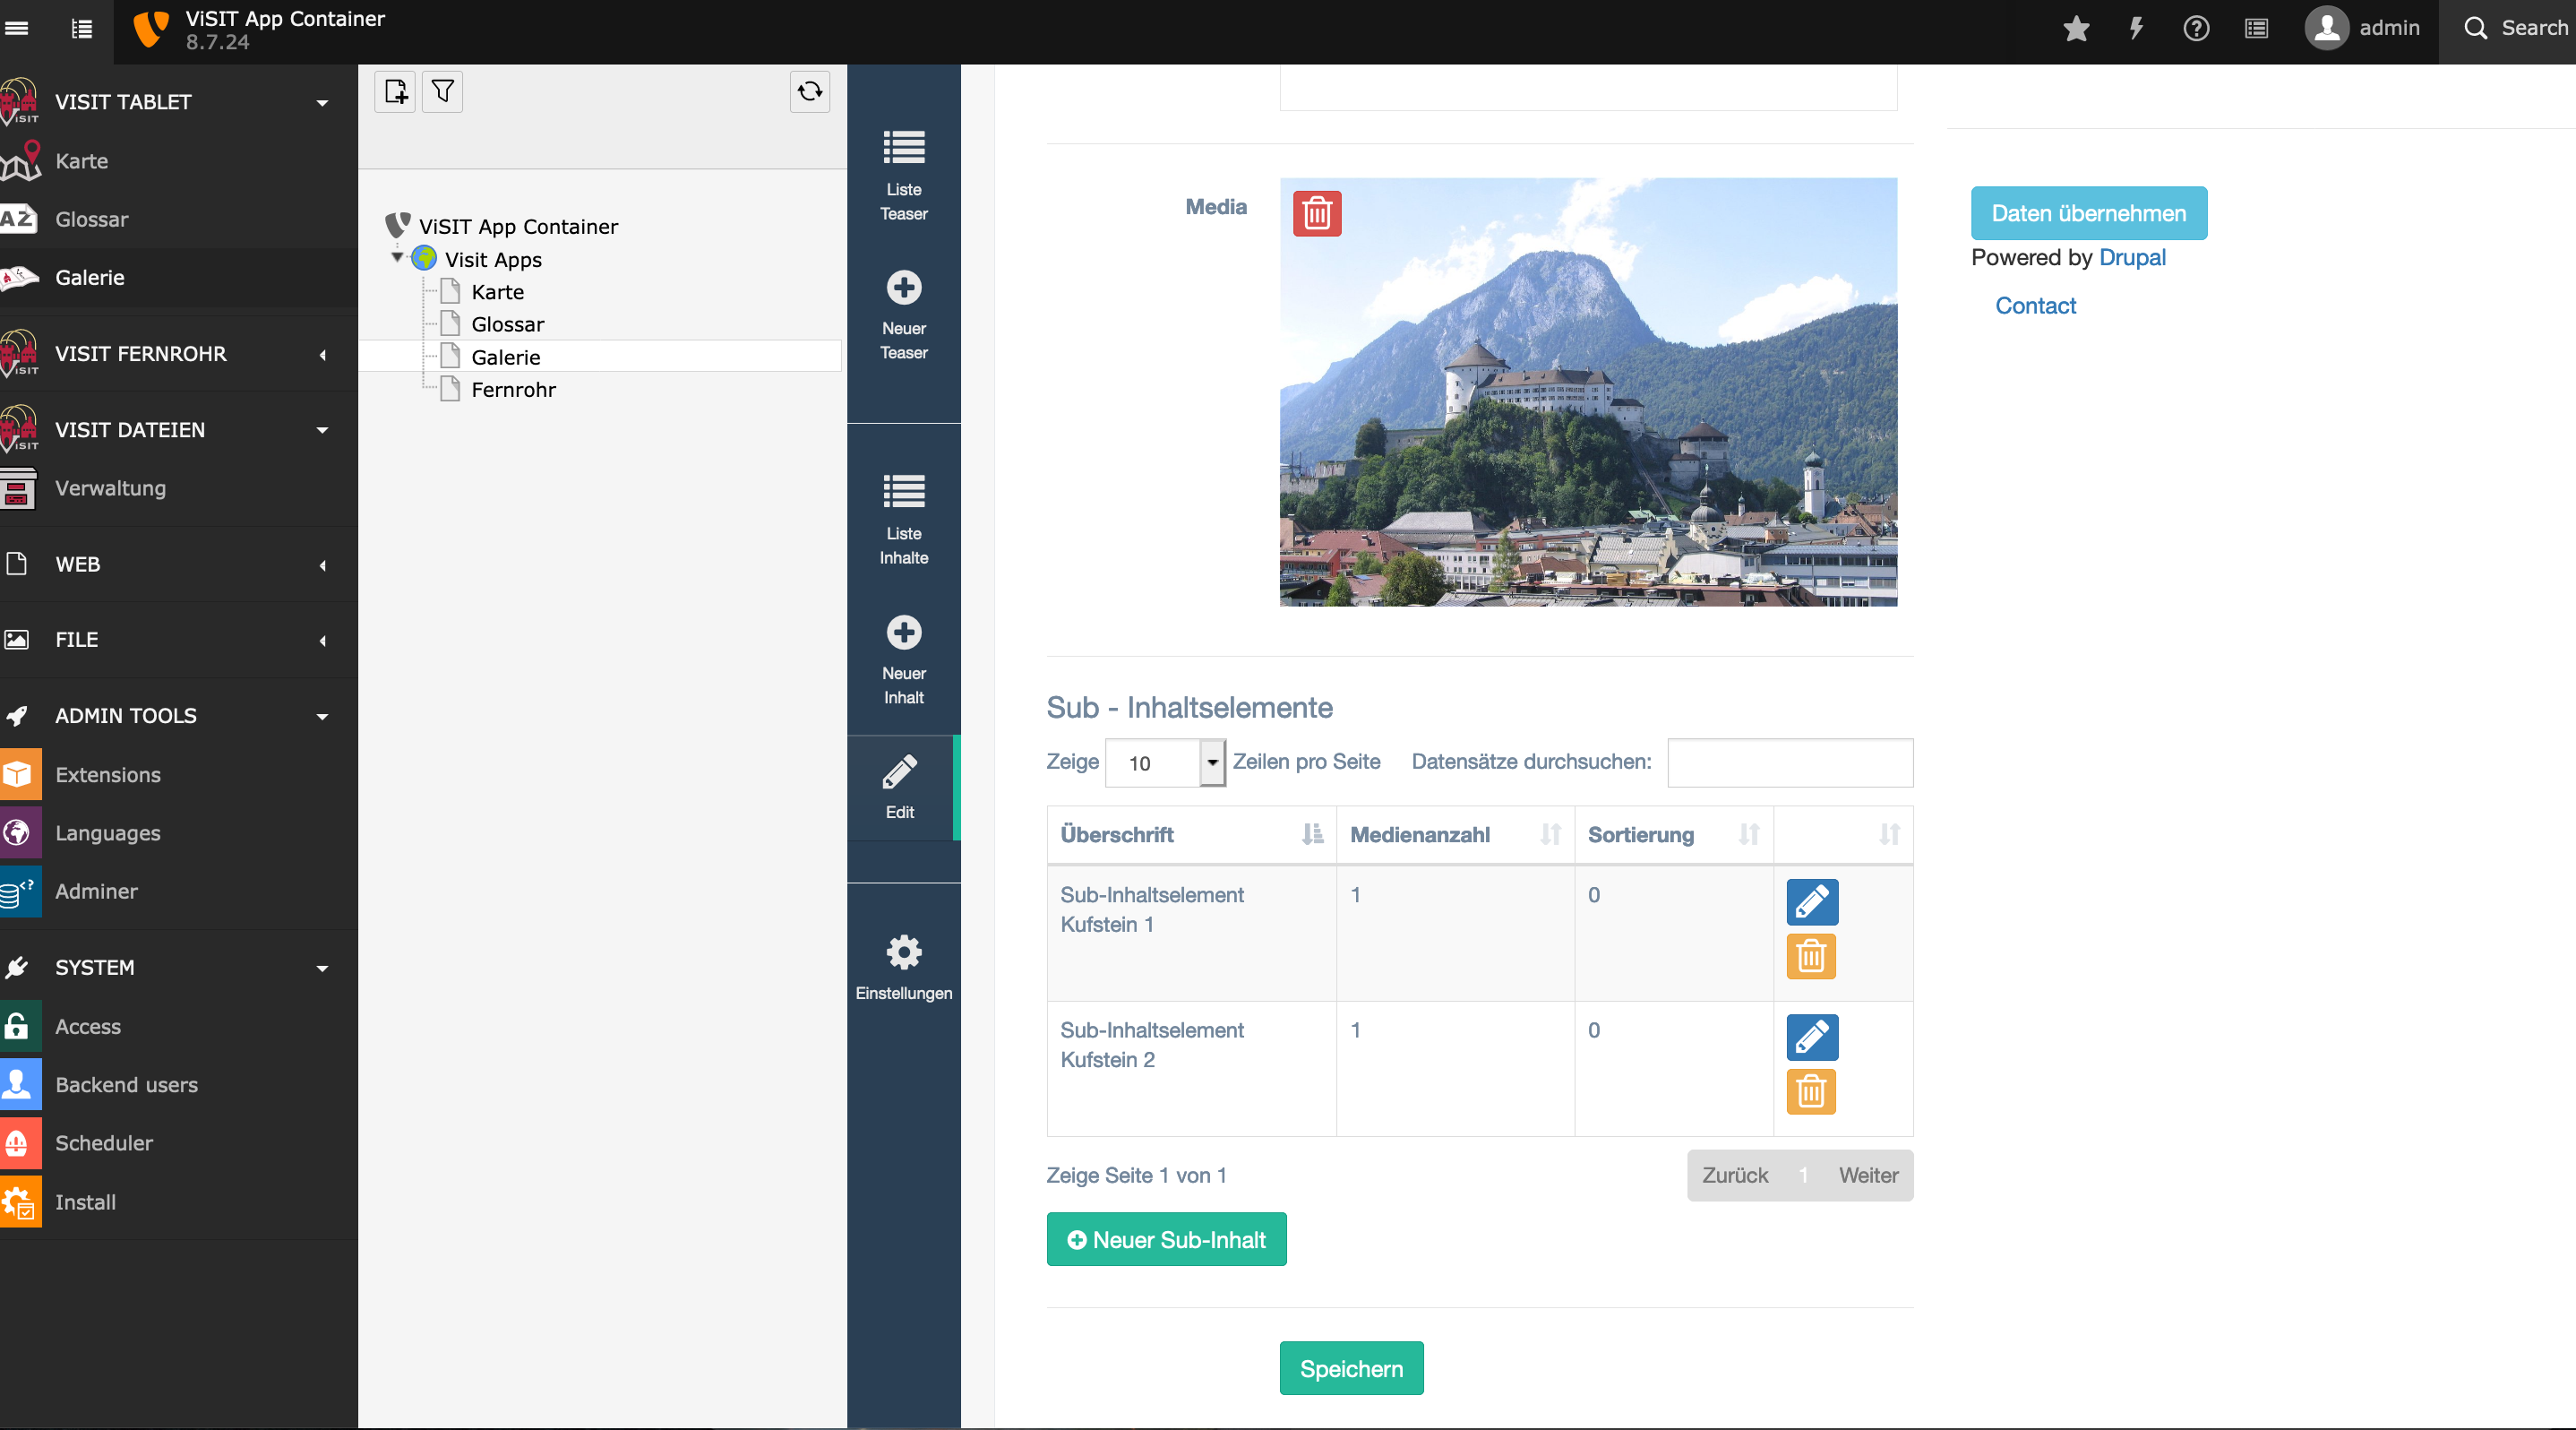
\includegraphics[width=12cm]{Figures/paula/galerie/anlegen_neuer_Sub_inhaltselemente.png}
\caption{Anlegen neuer Sub-Inhaltselemente zu einem bestehenden Inhaltselement}
\label{img:anlegen_neuer_Sub_inhaltselemente}
\end{figure}


\subsection{Erstellung der Teaser}

Für die Startseite müssen als nächstes die Teaser erstellt werden (siehe Abbildung \ref{img:layout_3er} und \ref{img:layout_6er}). Je nachdem welches Layout gewählt wurde, müssen entsprechend viele Teaser erstellt werden, also entweder 3 oder 6. 

Dazu zuerst aus den dunkelblauen Leiste \glqq Neuer Teaser\grqq{} auswählen und den Titel sowohl in Deutsch als auch in Englisch eintragen. Des Weiteren muss der Link zum entsprechenden Inhaltselement angegeben werden (siehe Abbildung \ref{img:erstellung_teaser}). 

\begin{figure}[ht!]
\centering
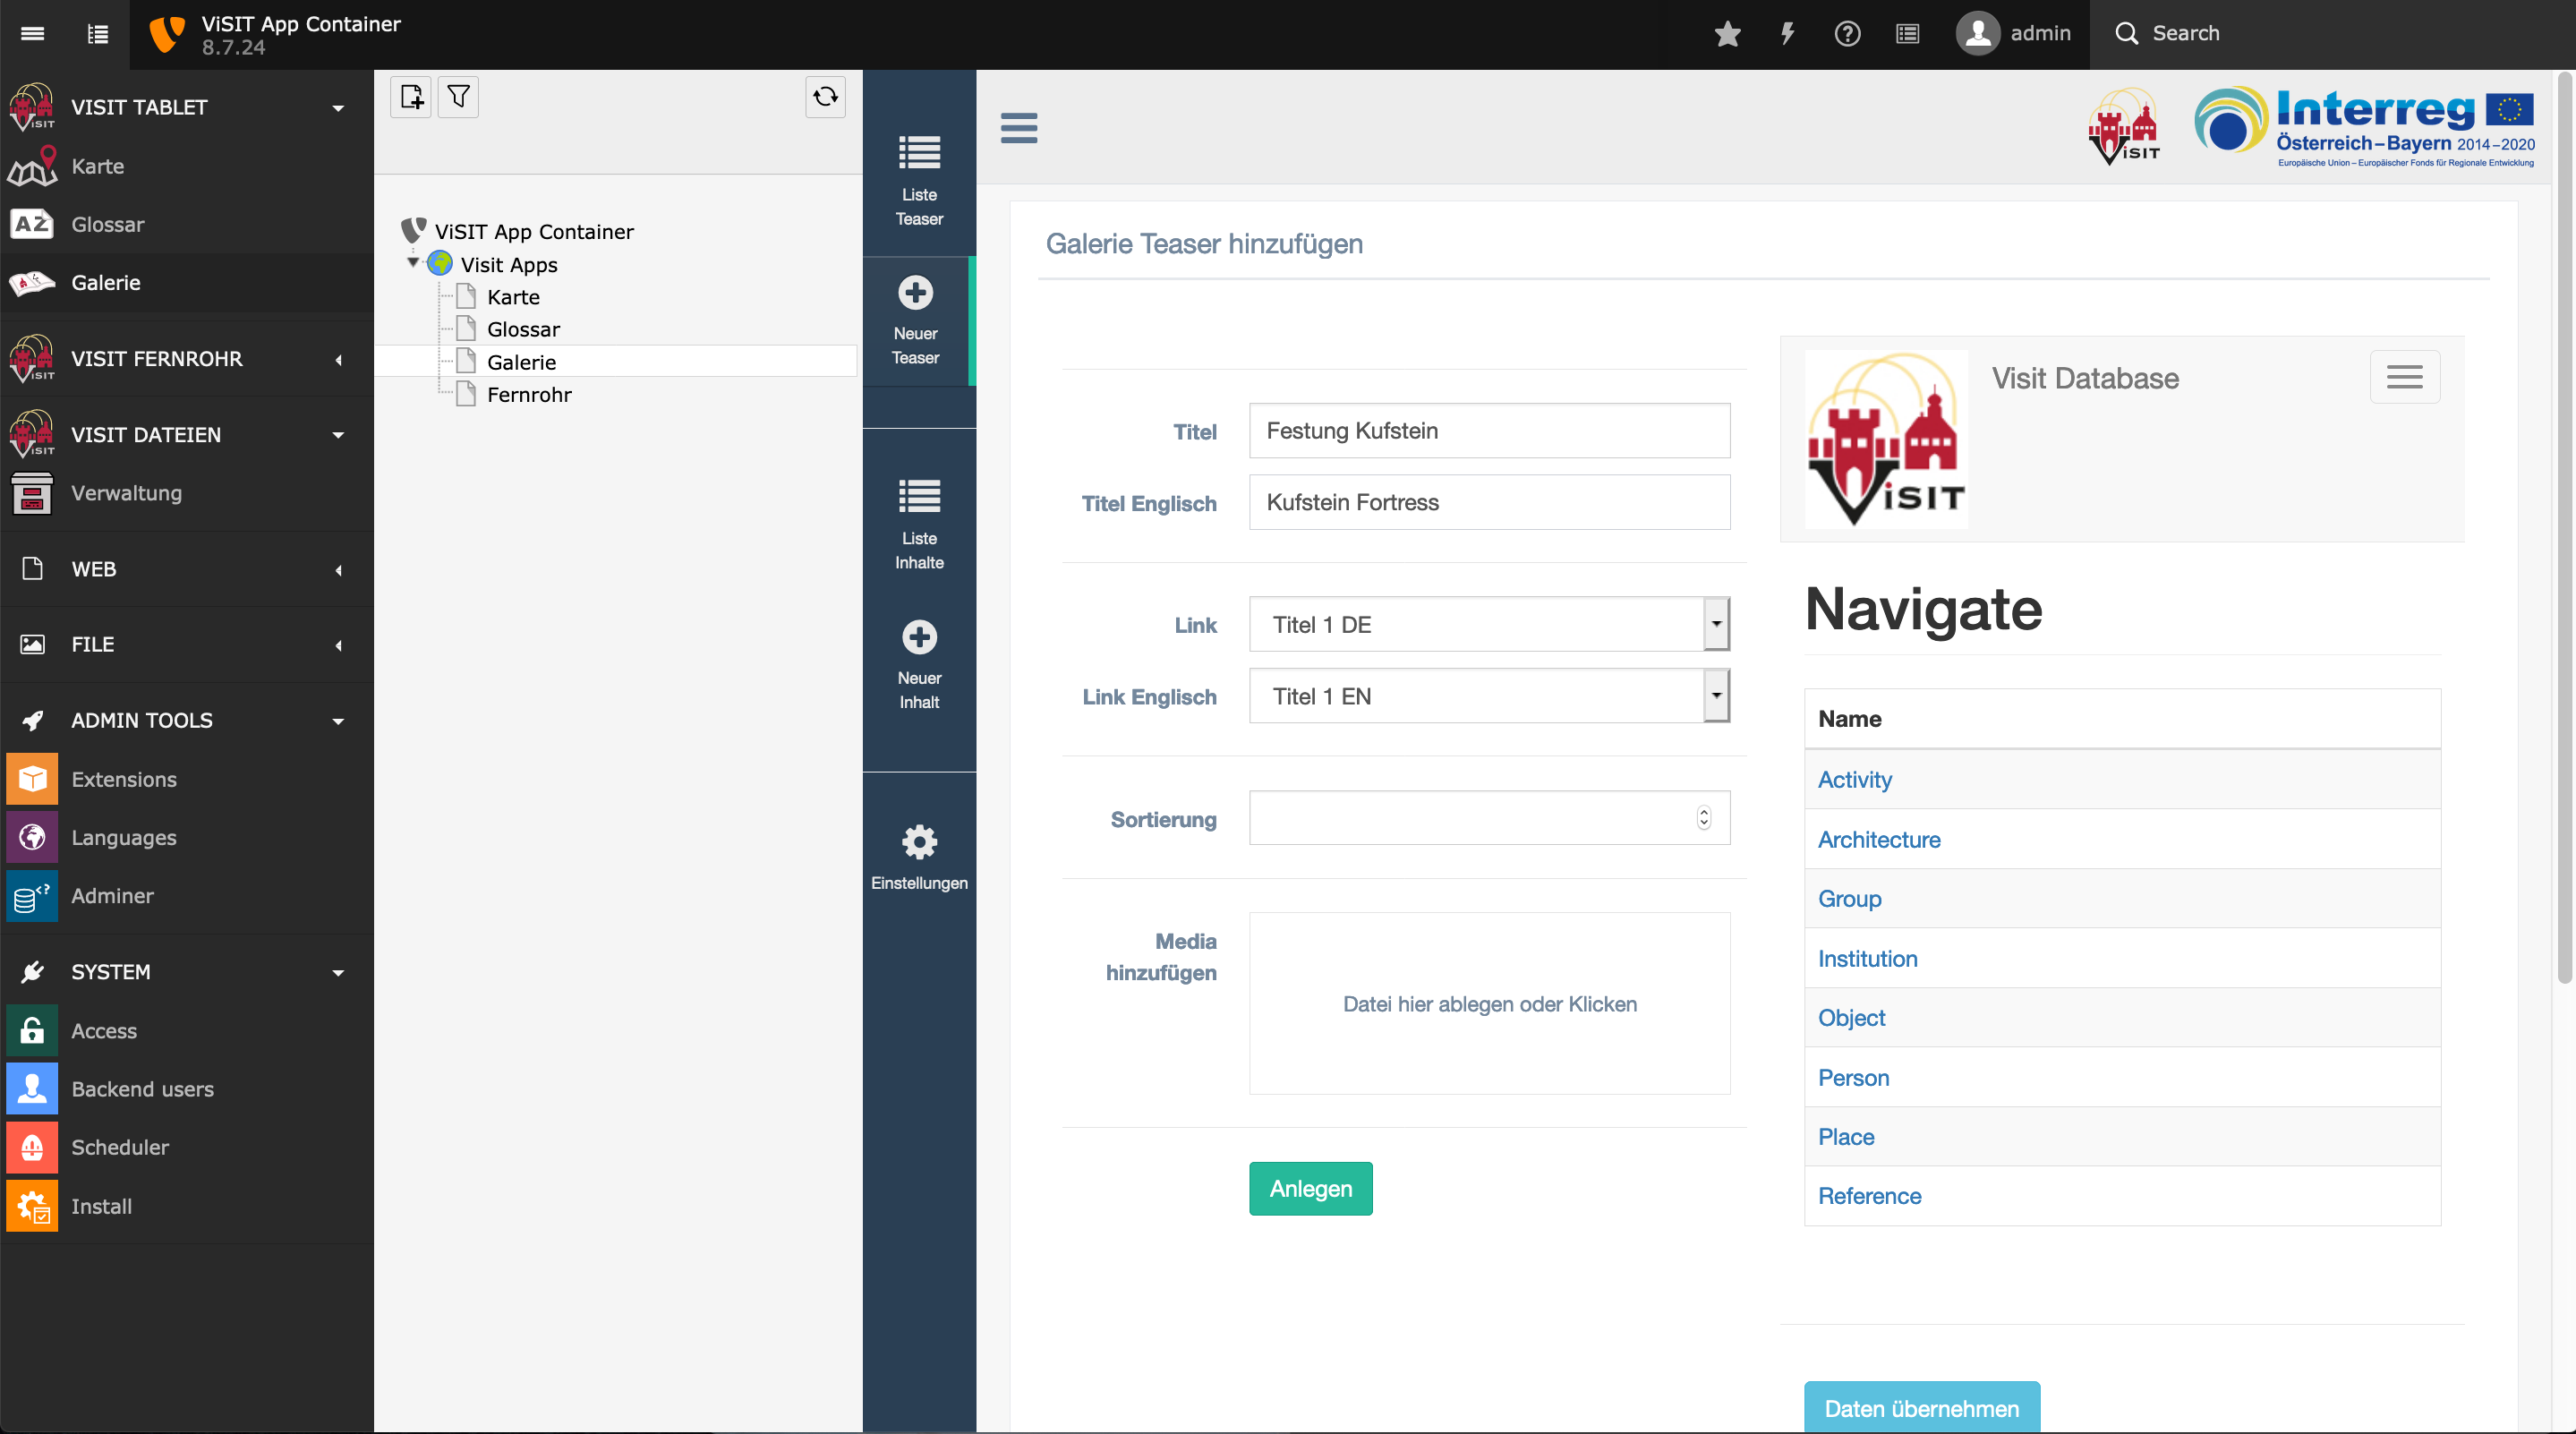
\includegraphics[width=12cm]{Figures/paula/galerie/erstellung_teaser.png}
\caption{Erstellung eines Teasers für die Startseite der Galerie-Applikation}
\label{img:erstellung_teaser}
\end{figure}

\subsection{Sortierung der Teaserelemente}

Die Sortierung der Teaser auf der Startseite kann manuell eingestellt werden. Die Reihung kann bei der Erstellung des Teasers angegeben werden (siehe Abbildung \ref{img:erstellung_teaser} bei Feld \glqq Sortierung\grqq{}). Hier kann über die Pfeiltasten eine Zahl ausgewählt werden, an der der Teaser auf der Startseite angezeigt wird. In der Abbildung \ref{img:sortierung_teaser} wird zuerst die Burg Kreuzenstein, dann die Festung Hohensalzburg und als dritter Teaser die Festung Kufstein angezeigt.

Wird bei allen Null angegeben, dann erscheinen die Teaser in der erstellten Reihenfolge.

\begin{figure}[ht!]
\centering
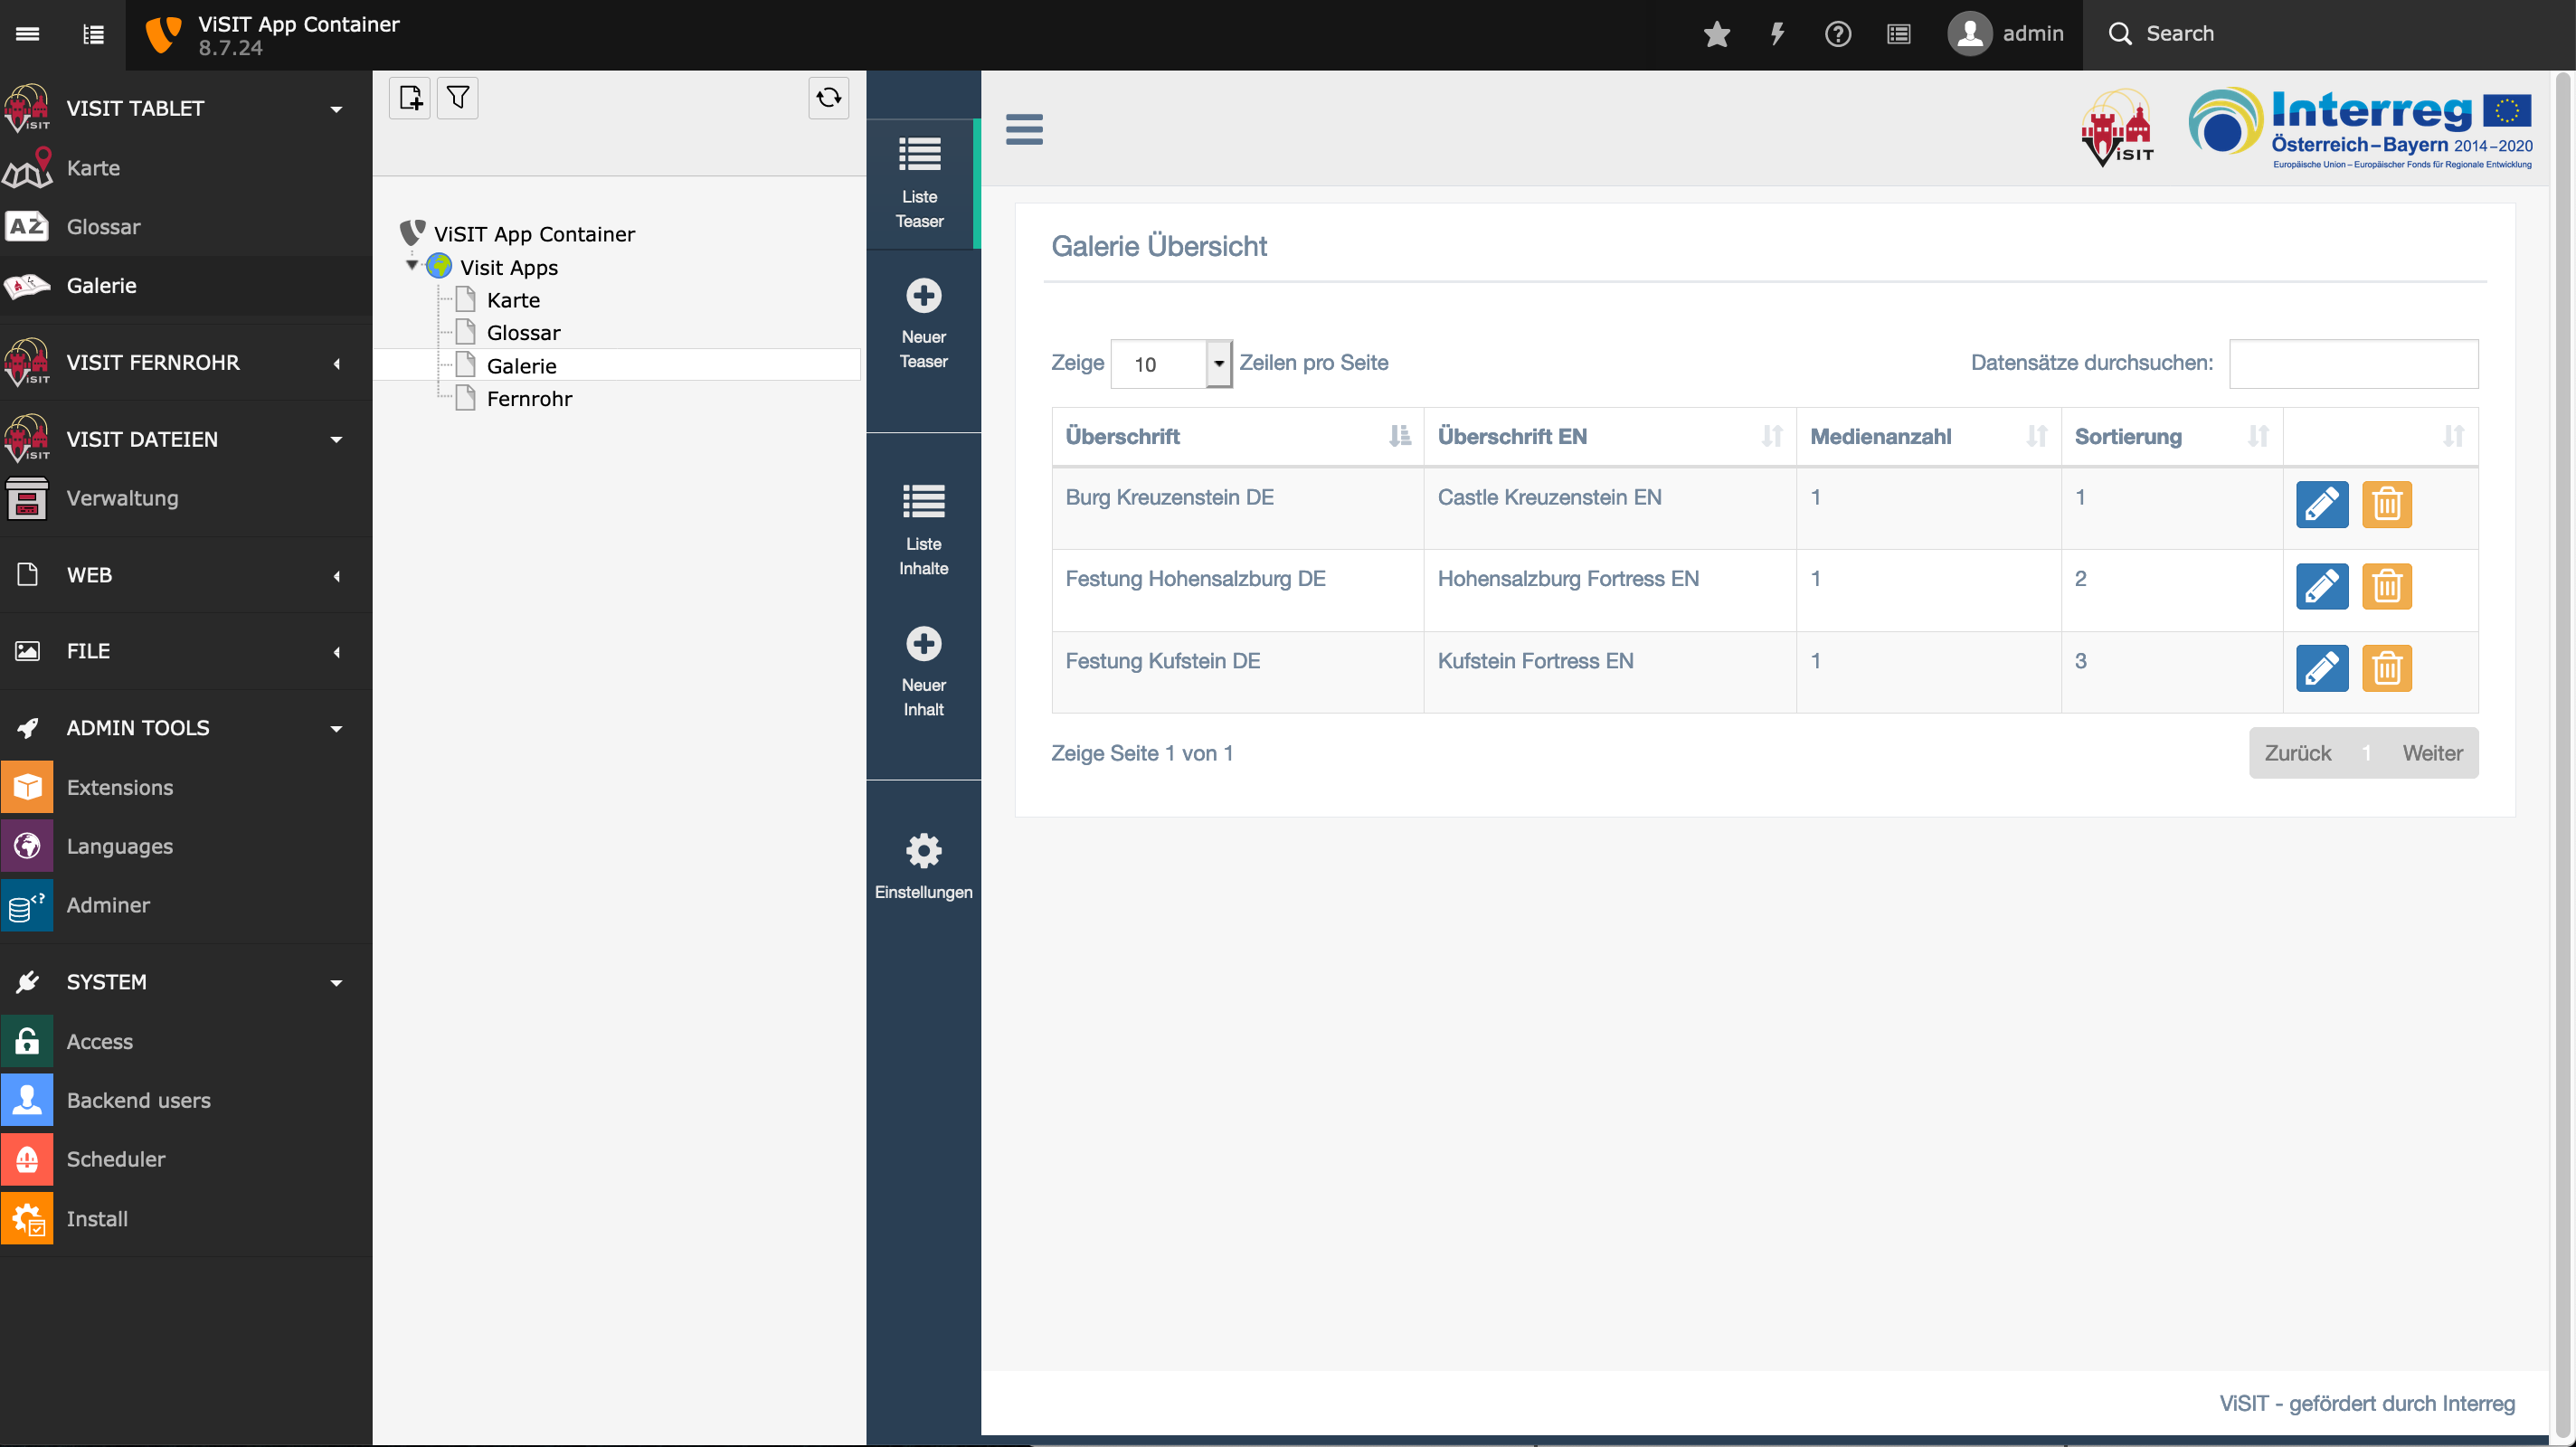
\includegraphics[width=12cm]{Figures/paula/galerie/sortierung_teaser.png}
\caption{Manuelle Sortierung der Teaserelemente auf der Startseite}
\label{img:sortierung_teaser}
\end{figure}


\subsection{Bearbeitung und Löschung Inhaltselementen, Sub-Inhaltselementen sowie Teasern}

Die Inhaltselemente, Sub-Inhaltselemente sowie Teaser können jederzeit bearbeitet oder gelöscht werden. Dies geht indem zuerst die jeweilige Listenansicht in der dunkelblauen Leiste ausgewählt wird (für Inhaltselemente beziehungsweise Sub-Inhaltselemente die \glqq Liste Inhalte\grqq{} und für Teaser die \glqq Liste Teaser\grqq{}). In weiterer Folge kann jedes einzelne Element (Zeile) einzeln bearbeitet oder gelöscht werden. Zum Bearbeiten auf das blaue Stiftsymbol auf der rechten Seite klicken, zum Löschen des gewünschten Objekts, den orangen Müllkübel.








\cleardoublepage


\section{Fernrohr}

Das Fernrohr ist für die Einrichtung die komplexeste Applikation.\\

Wenn durch das Fernrohr geschaut wird, sieht man eine Karte oder Landschaft. Auf dieser Karte oder Landschaft befinden sich sogenannte POI's (Point of Interest), das sind Punkte, die Informationen beinhalten. Jeder POI hat einen zuvor festgelegten Radius, welcher die Größe des POI festlegt. POI's können unterschiedliche Größen haben, bei jedem Punkt, der angelegt wird, muss der Radius des Punktes angegeben werden.\\

Das Fernrohr lässt sich nach rechts und links schwenken, sowie nach oben und unten bewegen. Wird ein POI mittig auf dem Screen anvisiert, dann vergrößert sich der Radius von diesem POI und der Inhalt wird auf dem ganzen Screen angezeigt. Handelt es sich dabei um ein Video, wird dieses direkt abgespielt. Die Videos haben eine leichte Transparenz, sodass die Karte im Hintergrund noch sichtbar ist.\\

Will man den Punkt verlassen, so muss das Fernrohr aus dem Radius des POI hinaus bewegt werden. Dann wird aus dem POI hinaus gezoomt und die darunter liegende Karte oder Landschaft wird wieder sichtbar. 

\subsection{Einpflegen der Daten in die Fernrohr-Applikation für Kuratoren}

Dieser Absatz gilt, wenn das Fernrohr bereits eingerichtet ist und nur ein neuer POI (Points of Interesst) hinzugefügt werden soll.\\

Dazu aus der Modulleiste links unter der Obergruppe VISIT FERNROHR POI's auswählen. Im linken Teil des Hauptfensters ist der Seitenbaum zu sehen und rechts befindet sich die Liste mit den bereits angelegten POI's (siehe Abbildung \ref{img:fernrohr_listenuebersicht}).\\

Als nächstes müssen in der dunkelblauen Leiste die \glqq Einstellungen\grqq{} ausgewählt und das Häckchen bei Kuratorenmodus gesetzt und gespeichert werden (siehe Abbildung \ref{img:fernrohr_einstellungen}). Danach kann bereits die Seite im Browser geöffnet werden. Dies geschieht über einen Rechtsklick auf \glqq Fernrohr\grqq{} im Seitenbaum und der Auswahl \glqq Show\grqq{} (siehe Abbildung \ref{img:fernrohr_browser_ansicht}). 



\begin{figure}[ht!]
\centering
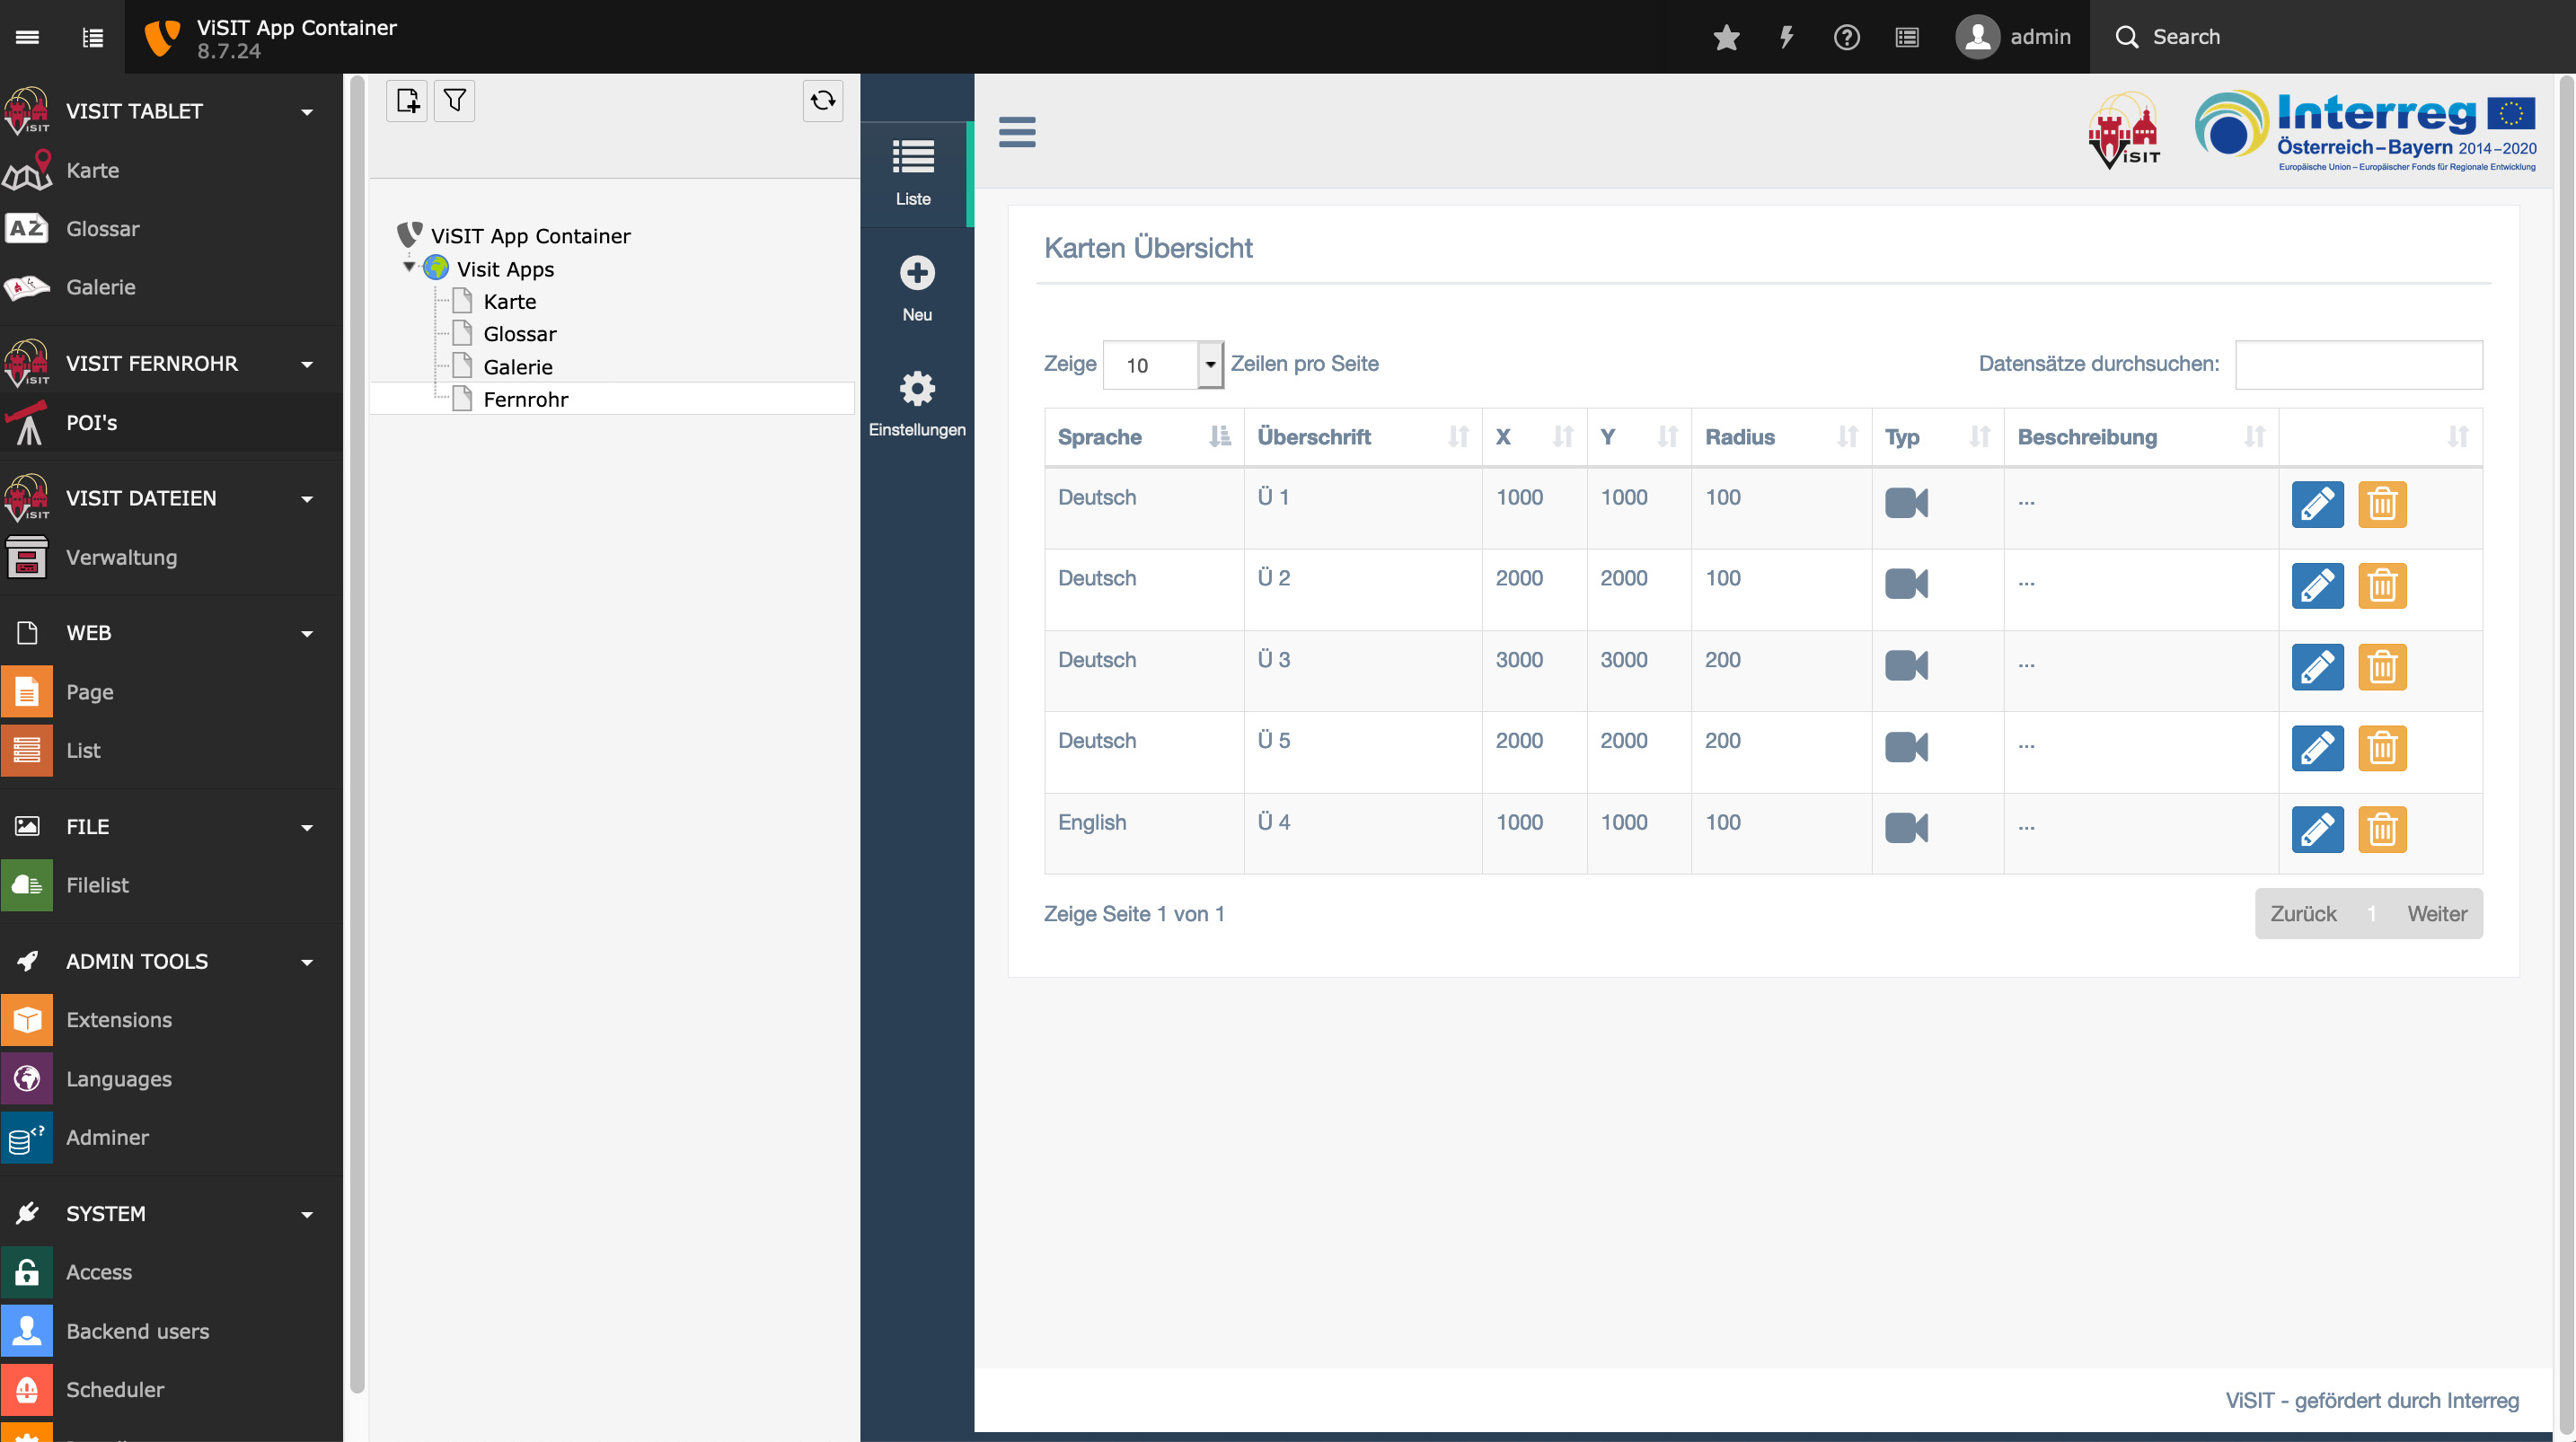
\includegraphics[width=12cm]{Figures/paula/fernrohr/fernrohr_liste.png}
\caption{Fernrohr - Übersicht über alle angelegten POI}
\label{img:fernrohr_listenuebersicht}
\end{figure}

\begin{figure}[ht!]
\centering
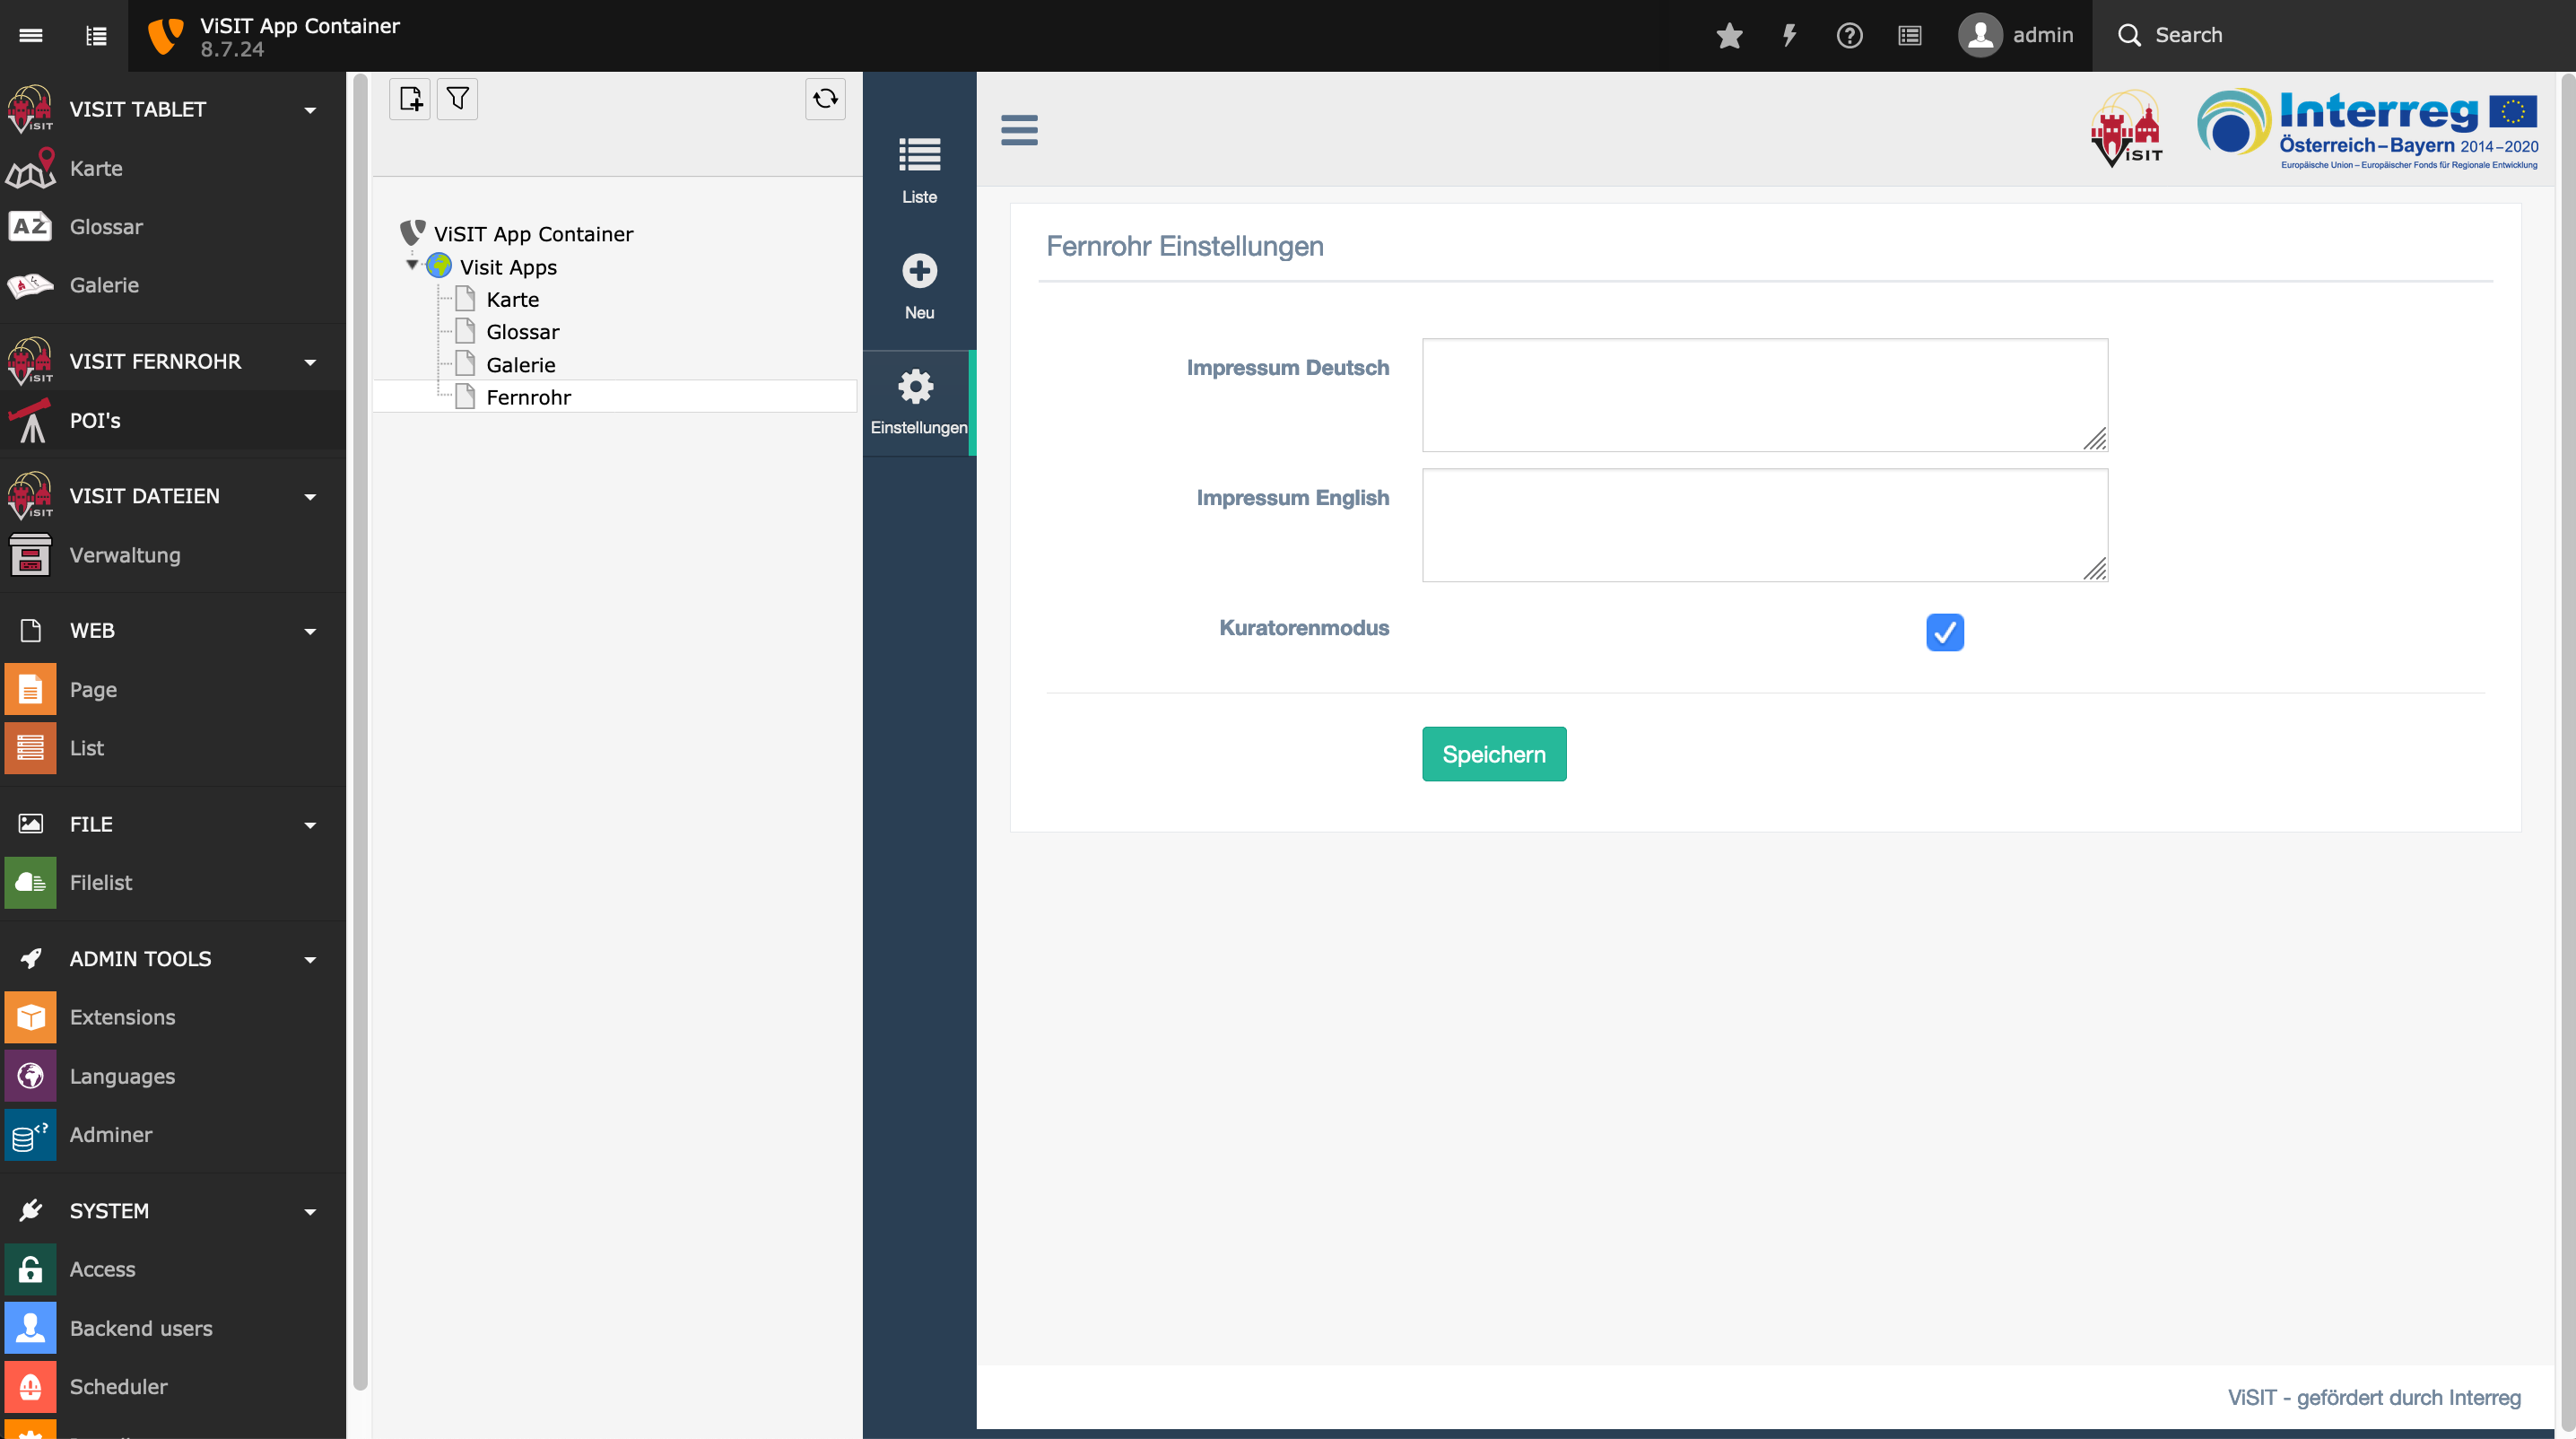
\includegraphics[width=12cm]{Figures/paula/fernrohr/fernrohr_einstellungen.png}
\caption{Einstellungen - Kuratorenmodus}
\label{img:fernrohr_einstellungen}
\end{figure}

\begin{figure}[ht!]
\centering
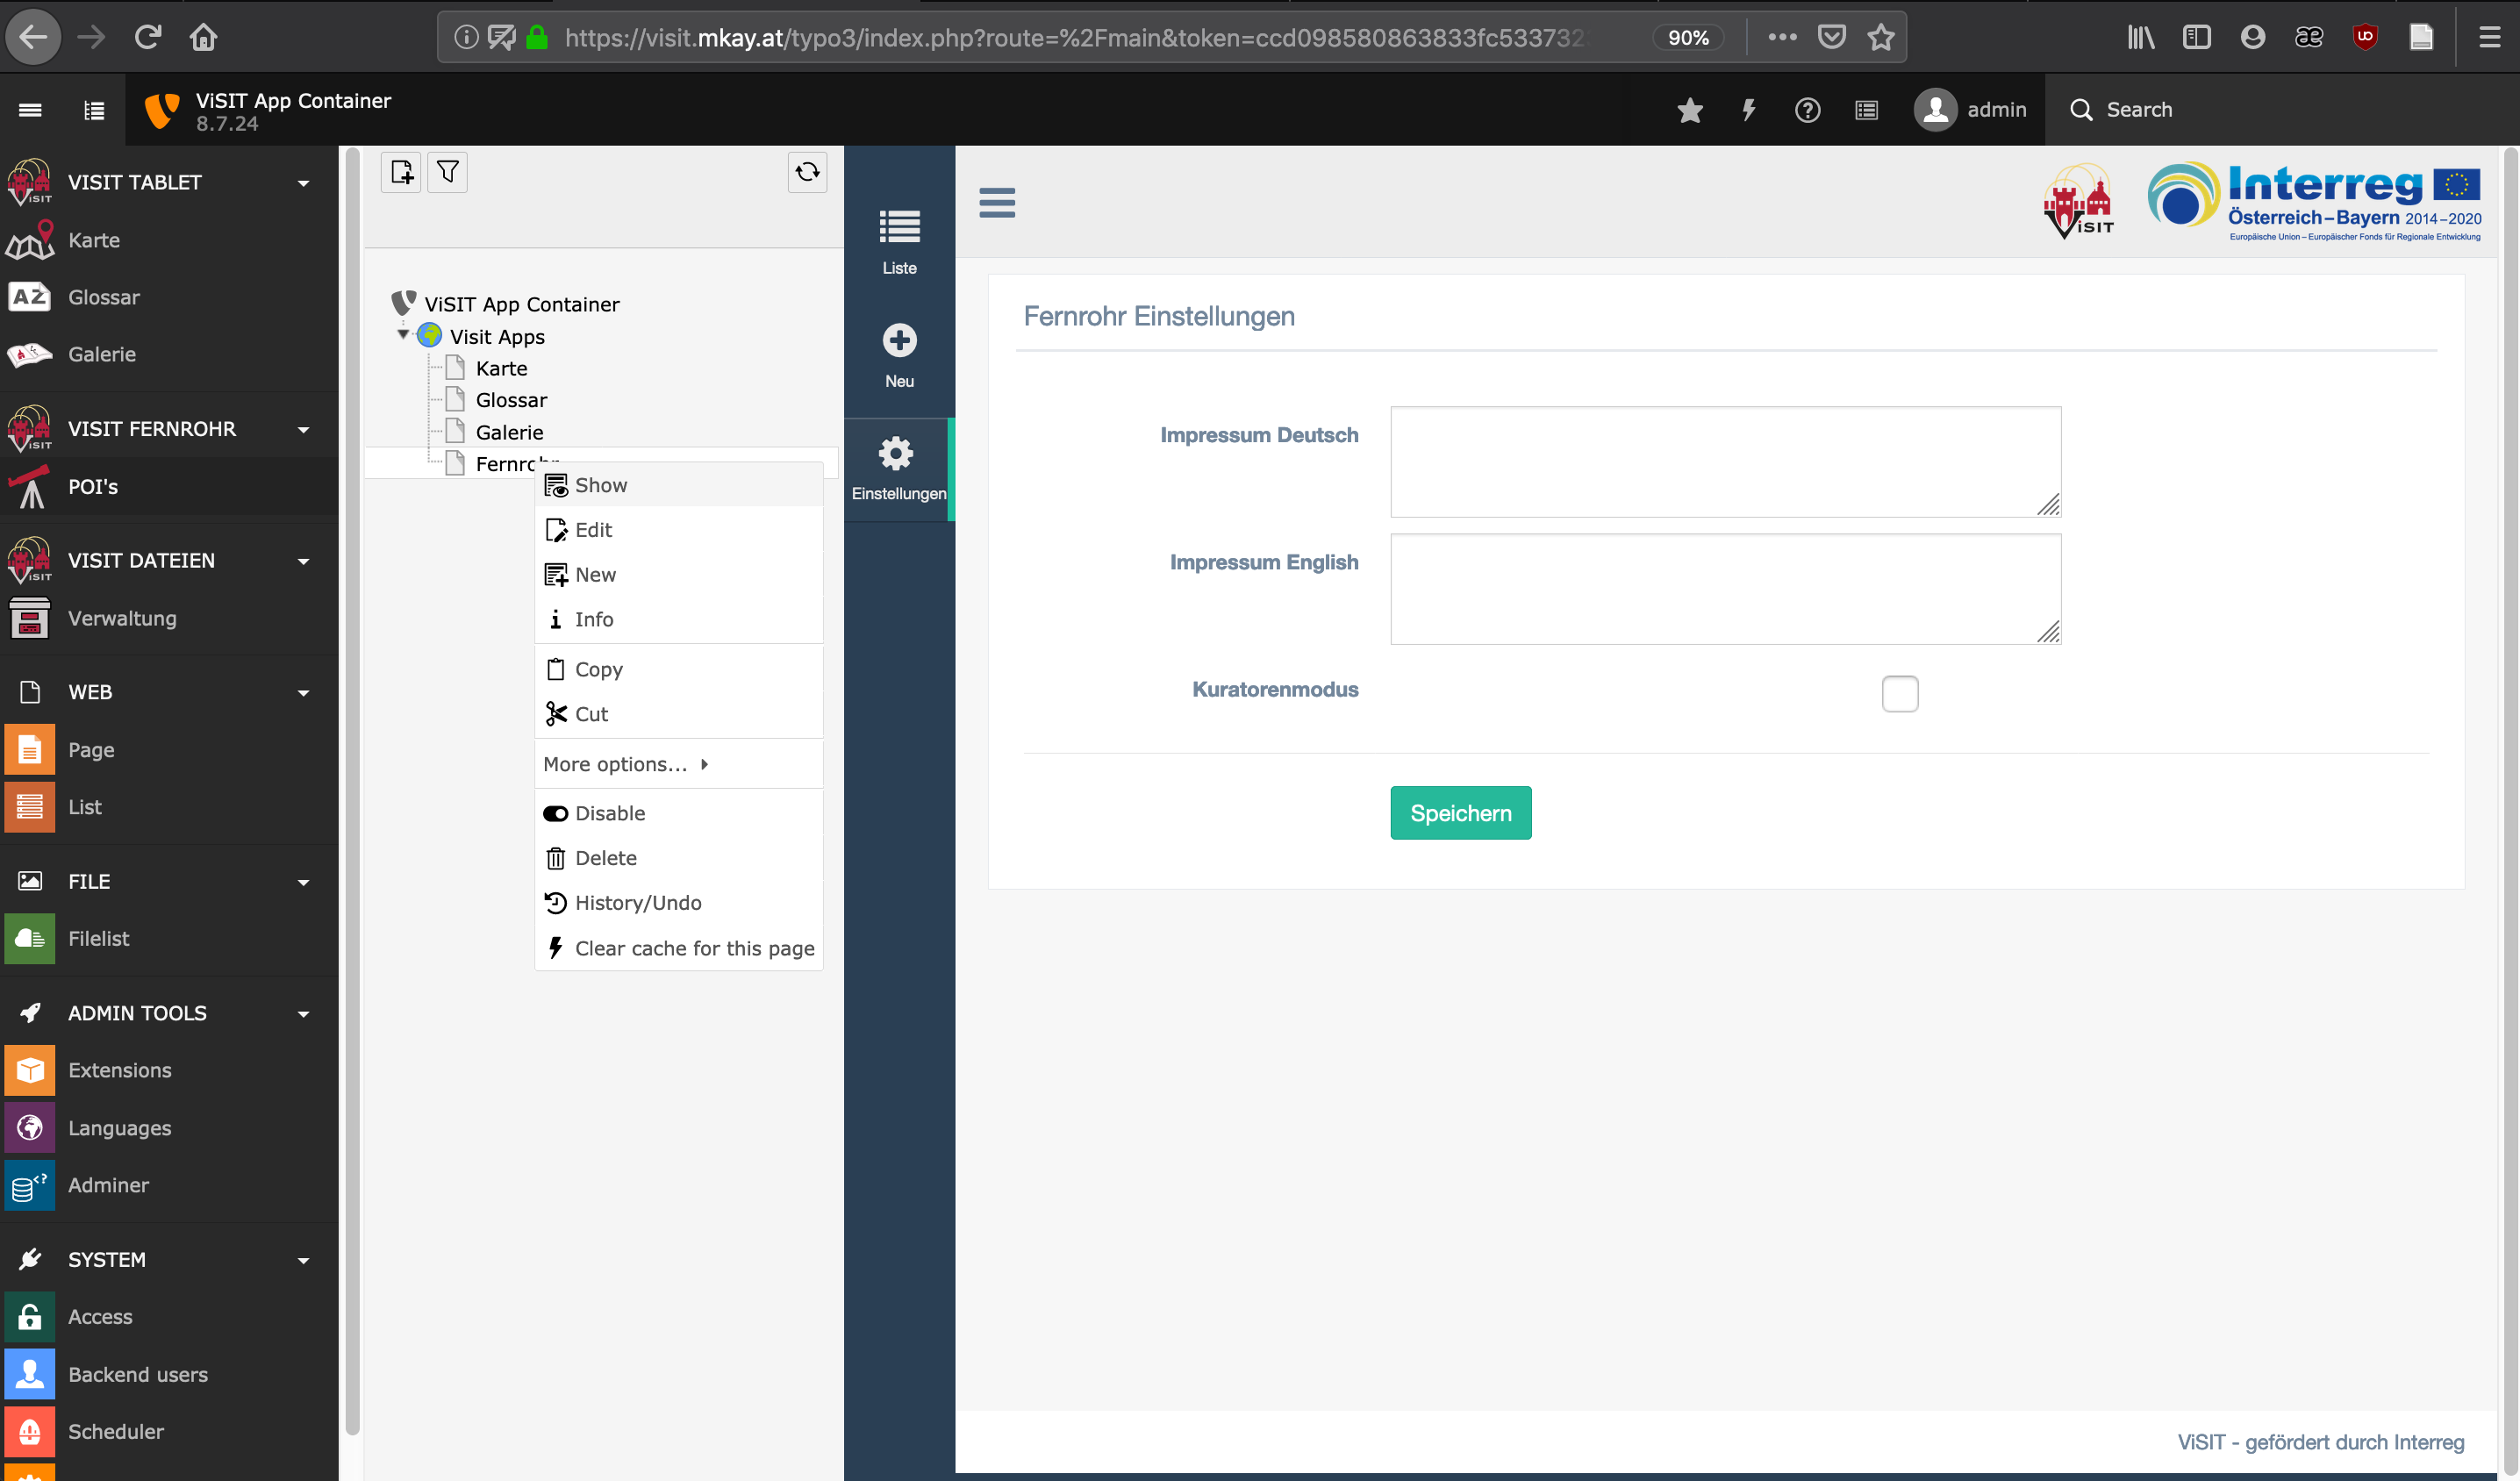
\includegraphics[width=12cm]{Figures/paula/fernrohr/fernrohr_ansicht_browser.png}
\caption{Web-Ansicht öffnen}
\label{img:fernrohr_browser_ansicht}
\end{figure}


\subsubsection{Auslesen der x- und y-Koordinaten}

Im Browser öffnet sich nun die Webseite und im oberen rechten Eck ist das sogenannte Kuratorenkästchen eingeblendet (siehe Abbildung \ref{img:kuratorenkaestchen}). In diesem werden die x- und y-Koordinaten der aktuellen Position des Fernrohrs (der Mittelpunkt des Sichtfeldes) und die bereits bestehenden Punkte angezeigt. Der blaue Hindergrund in der Abbildung \ref{img:kuratorenkaestchen} wird im realen Einsatz die Karte oder Landschaft sein, auf welcher sich die POI's befinden.
Hat man den Punkt ausgewählt an welchem das neue Bild oder Video angezeigt werden soll, dann müssen die Werte der x- und y-Koordinaten notiert werden.\\

Des Weiteren sind in der Ansicht auch die Sprachauswahlmöglichkeiten sichtbar. Fährt der Besucher auf das POI mit der Deutschen Flagge, dann wird der Inhalt aller anderen POI's auf Deutsch angezeigt. Fährt der Besucher auf die Britische Flagge, werden die Inhalte aller POI's auf Englisch angezeigt. Daneben, als drittes POI, befindet sich das Impressum, welches in der gewählten Sprache erscheint, wenn der Besucher diesen POI anvisiert.\\

Sobald eines dieser POI anvisiert wird - dieses sich also im Mittelpunkt des Sichtfensters befindet - wird der Radium des POI's größer und der Text oder das Video (Video wird automatisch abgespielt, der Besucher muss nicht mehr auf Start drücken) werden angezeigt. 
Will der Besucher das ausgewählte POI wieder verlassen, muss er das Fernrohr bewegen und den Punkt verlassen. So gelangt er wieder zu der Karte oder Landschaft.

\begin{figure}[ht!]
\centering
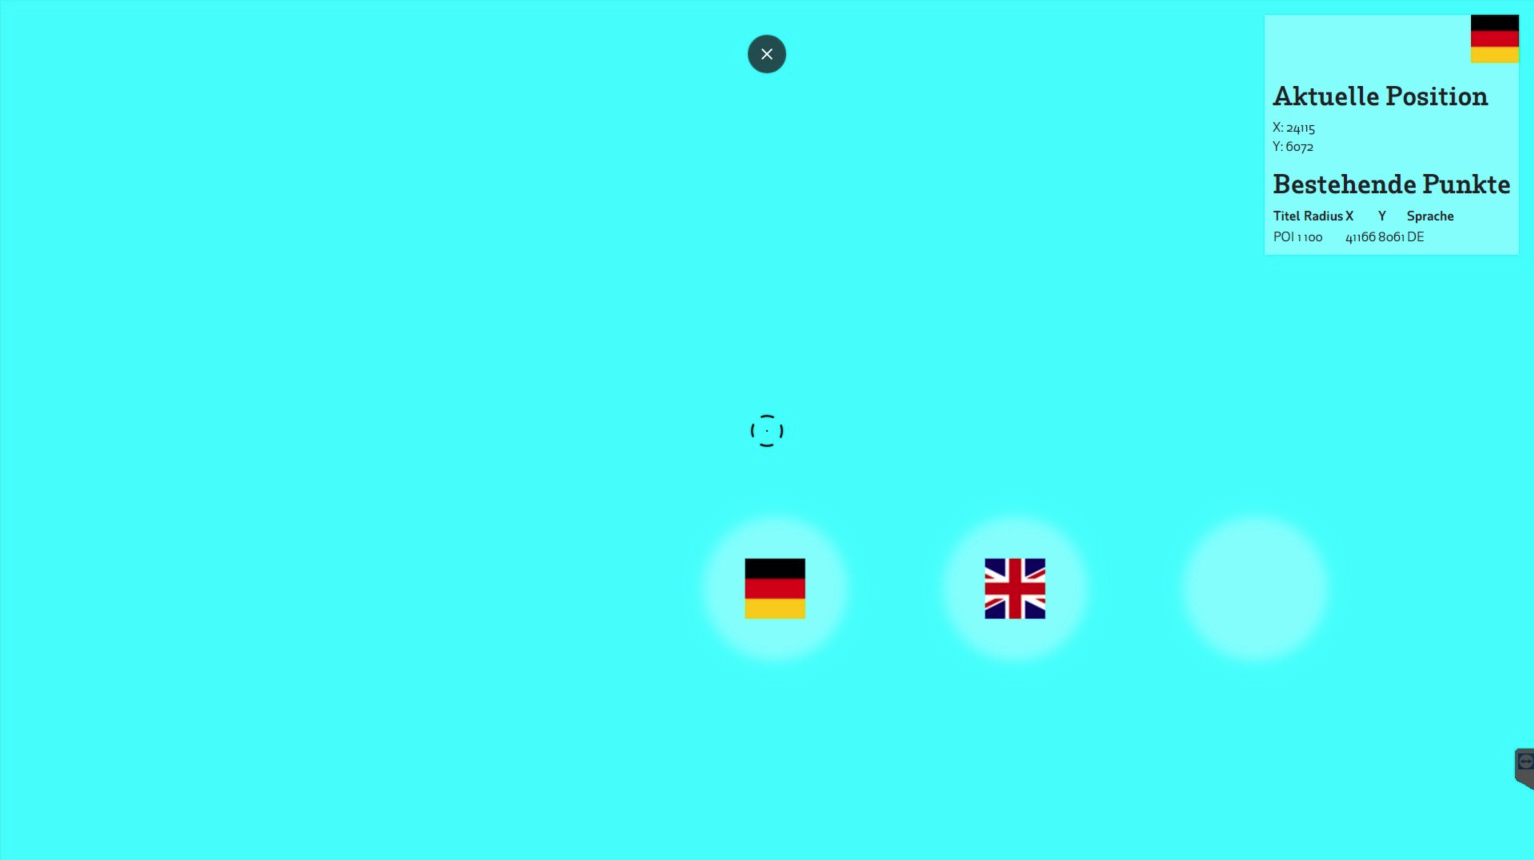
\includegraphics[width=12cm]{Figures/paula/fernrohr/kuratorenkaestchen.png}
\caption{Kuratorenkästchen in der oberen rechten Ecke}
\label{img:kuratorenkaestchen}
\end{figure}

\subsubsection{Anlegen eines neuen Kartenelements}

Als nächstes wählt man aus der dunkelblauen Leiste \glqq Neu\grqq{} aus. Hier kann ein neues Kartenelement hinzugefügt werden. Als erstes wird die gewünschte Sprache ausgewählt.

Die beiden Überschriften werden nur benötigt, wenn es sich um einen Texttyp (also zum Beispiel ein Bild und dazu ein Text zum Lesen) handelt. Zum Texttyp gab es keine Designvorlage, dies wurde lediglich Vollständigkeit halber implementiert, grundsätzlich ist die Fernrohr-Applikation dafür da, Fullscreen Videos abzuspielen. Sollte ein Texttyp verlangt werden, muss das entsprechende Design implementiert werden.\\

Bei Videos reicht nur eine Überschrift. Als nächstes muss die Position eingetragen werden. Hier müssen die zuvor notierten x- und y-Koordinaten aus dem Kuratorenkästchen eingetragen werden (siehe Abbildung \ref{img:fernrohr_x_u_y_koordinaten}). Handelt es sich um ein Fullscreen Video, dann muss das Häckchen daneben gesetzt werden. Sollte es sich um einen Texttyp handeln, dann können optional noch Medien hinzugefügt werden.

\subsubsection{Größe (Radius) der POI's}

Die Größe der POI's muss beim Anlegen eines neuen Kartenelements angegeben werden. Hier muss geschaut und ausprobiert werden, welche Größe als passend empfunden wird. Je größer die Zahl, desto größer wird der Punkt auf der Karte angezeigt.

\begin{figure}[ht!]
\centering
\includegraphics[width=12cm]{Figures/paula/fernrohr/fernrohr_x_u_y_koordinaten.png}
\caption{Eintragen der x- und y-Koordinaten des neuen POI}
\label{img:fernrohr_x_u_y_koordinaten}
\end{figure}


\subsubsection{Erstellung des Impressums für die Fernrohr-Applikation}

Das Impressum ist in den Einstellungen der Fernrohr-Applikation zu finden. Dazu muss aus der dunkelblauen Leiste auf \glqq Einstellungen\grqq{} geklickt werden (siehe Abbildung \ref{img:fernrohr_einstellungen}). Hier kann der Text des Impressums sowohl auf Englisch als auch auf Deutsch eingegeben werden. Nach dem Befüllen müssen die Daten gespeichert werden.


\subsubsection{Ansicht der Benutzer des Fernrohrs ohne des Kuratorenkästchens}

Für das Einpflegen der Daten war der Kuratorenmodus in den Fernrohr Einstellungen aktiviert. Ist man mit dem Einpflegen der Daten fertig und möchte die Ansicht haben, die die Benutzer haben werden, dann muss anschließend das Häckchen vom Kuratorenmodus entfernt werden.
Dies ist wieder in den Einstellungen des Fernrohrs zu finden. Nach der Entfernung des Häckchens kann die Seite mittels Rechtsklick auf \glqq Fernrohr\grqq{} und der Auswahl \glqq Show\grqq{} im Browser angezeigt werden. Jetzt ist das Kuratorenkästchen nicht mehr zu sehen, stattdessen befindet sich die Flagge der ausgewählten Sprache im oberen rechten Eck.


\subsection{Einrichtung des Fernrohrs durch TYPO3-Administratoren}

Die Einrichtung des Fernrohrs kann nur durch den TYPO3-Administrator erfolgen.\\

Dazu als ersten Schritt das Fernrohr im Seitenbaum auswählen und dann in der Modulleiste links unter der Obergruppe WEB \glqq List\grqq{} auswählen. Danach im Page Content-Kästchen das Stiftsymbol \glqq Edit record\grqq{} auswählen (siehe Abbildung \ref{img:fernrohr_einstellungen} rot eingerahmtes Symbol). Im Arbeitsbereich erscheint \glqq Edit Page Content on page \glqq Fernrohr\grqq{}\grqq{}, hier im Raster die \glqq Plugins\grqq{} auswählen (siehe Abbildung \ref{img:fernrohr_plugin} rot eingerahmter Bereich). Jetzt muss noch der Debugmodus aktiviert werden, dazu das Häckchen im entsprechenden Kästchen setzen (siehe Abbildung \ref{img:fernrohr_plugin} blau eingerahmt). Im nächsten Schritt muss der aktivierte Debugmodus gespeichert werden. Dies geschieht mit einem Klick auf das Disketten-Symbol im oberen Teil des Arbeitsbereichs (siehe Abbildung \ref{img:fernrohr_plugin} grün eingerahmt).\\


Wenn jetzt die Web-Ansicht über Rechtsklick auf Fernrohr im Seitenbaum und \glqq Show\grqq{} (siehe Abbildung \ref{img:fernrohr_webansicht_oeffnen}) geöffnet wird, dann wird rechts oben ein großes Kästchen mit einigen Daten sichtbar (siehe Abbildung \ref{img:fernrohr_webansicht_debugmodus}, der blaue Hintergrund ist im Produktivbetrieb eine Landkarte oder Landschaft).\\


\begin{figure}[ht!]
\centering
\includegraphics[width=12cm]{Figures/paula/fernrohr/einrichtung_fernrohr/fernrohr_liste_uebersicht.png}
\caption{Einstellungen des Fernrohrs}
\label{img:fernrohr_einstellungen}
\end{figure}

\begin{figure}[ht!]
\centering
\includegraphics[width=12cm]{Figures/paula/fernrohr/einrichtung_fernrohr/fernrohr_plugin_einstellungen.png}
\caption{Das Plugin des Fernrohrs}
\label{img:fernrohr_plugin}
\end{figure}

\begin{figure}[ht!]
\centering
\includegraphics[width=12cm]{Figures/paula/fernrohr/einrichtung_fernrohr/fernrohr_web_ansicht.png}
\caption{Web-Ansicht öffnen}
\label{img:fernrohr_webansicht_oeffnen}
\end{figure}

\begin{figure}[ht!]
\centering
\includegraphics[width=12cm]{Figures/paula/fernrohr/einrichtung_fernrohr/fernrohr_web_ansicht1.png}
\caption{Web-Ansicht der Fernrohr-Webseite im aktivierten Debugmodus}
\label{img:fernrohr_webansicht_debugmodus}
\end{figure}



Erklärungen zu den einzelnen Werten:\\

\subsubsection{Encoder Offset X (RawX) und Encoder Offset Y (RawY)}

Die \textbf{Raw-Werte} geben die absolute Position des Drehgebers an. Diese Drehgeber sind mechanisch mit dem Fernrohrkopf verbunden und ermitteln die momentane Ausrichtung des Kopfes. Es wird die vertikale Position als X und die horizontale Position als Y erfasst. Die Werte sind abnehmend bei einer Rotation gegen den Uhrzeigersinn und Bewegung nach oben. 
Da die Verbindung zwischen Drehgeber und Kopf varrieren kann, sind die initialen Werte der Drehgeber nicht aussagekräftig. Um eine einfache Handhabung zu ermöglichen, können diese Werte genullt werden - links oben sollte sich dann der Nullpunkt befinden. Um diese Raw-Werte zu nullen wird ein Offset angewendet. Dieser Offset wird von den tatsächlichen Drehgeberwerten (Raw) subtrahiert. 

Später werden die Werte auf Null gesetzt, damit es einfacher wird, mit den Werten zu arbeiten. Somit sind bei der weiteren Arbeit ganz oben links die Koordinaten 0/0.\\


\textbf{Zum Eintragen der Werte:}\\

Von dem in dem Kästchen (siehe Abbildung \ref{img:fernrohr_webansicht_debugmodus}) angegebenen \textbf{RawX-Wert} muss zirka 1000 abgezogen werden. Dies ist aus dem Grund, dass das Fernrohr noch ein kleines Stück nach oben und links gedrückt werden kann. Sollte der \textbf{RawX-Wert} zum Beispiel 42162 sein, dann sollte 41000 in den Plugin-Optionen im Backend eingetragen werden (siehe Abbildung \ref{img:x_y_werte}, blau eingerahmt).\\
\\

\begin{figure}[ht!]
\centering
\includegraphics[width=12cm]{Figures/paula/fernrohr/einrichtung_fernrohr/x_y_werte.png}
\caption{Einzutragende Daten in den Plugin Optionen}
\label{img:x_y_werte}
\end{figure}


Das gleiche wird mit dem \textbf{Raw-Y} gemacht. Sollte \textbf{Raw-Y} zum Beispiel 11623 sein, dann wird 11000 in die Plugin-Optionen eingetragen.


\subsubsection{App Start X (CurrentX) und App Start Y (CurrentY)}

\textbf{App Start X} und \textbf{App Start Y} geben den oberen linken Wert an, wo die Applikation anfängt. Das Fernrohr lässt einen Bewegungsradius von 180 Grad zu, für die Applikation werden jedoch nicht die vollen 180 Grad ausgenutzt sondern zum Beispiel 90 Grad. Mit den Werten \textbf{App Start X} und \textbf{App Start Y} gibt man den Startpunkt der Applikation an. Es sind also die Koordinaten von dem oberen linken Eck, wo die Landkarte oder Landschaft beginnen soll. Der entsprechende Wert muss im Backend in den Plugin Optionen eingetragen werden (siehe Abbildung \ref{img:x_y_werte}, grün eingerahmt).

\subsubsection{App End X (CurrentX) und App End Y (CurrentY)}

Wie bei App Start X und Y der Anfang der Applikation angegeben wurde, so muss auch das untere rechte Eck, also das Ende der Applikation angegeben werden. Das Ende der Applikation wird mit dem \textbf{App End X} und \textbf{App End Y} angegeben. Diese Werte müssen ebenfalls im Backend eingetragen werden (siehe Abbildung \ref{img:x_y_werte}, rot eingerahmt).\\

Durch die Angabe der \textbf{App Start X und Y-Werte} und der \textbf{App End X und Y-Werte} entsteht ein Rechteck zwischen den Koordinaten, in welchem die Landkarte oder Landschaft angezeigt wird.


\subsubsection{Überblendende Ebene aktivieren}

Das Bild, wenn durch das Fernrohr geschaut wird, besteht aus zwei Lagen. Die erste Lage ist die Landkarte oder Landschaft. Auf dieser ersten Lage kann eine zweite Lage (ein sogenanntes Overlay) gelegt werden. Bei dem Overlay handelt es sich um die Icons für die Sprache und das Impressum. Wird hier das Häckchen gesetzt, so werden die Icons über den POI's sichtbar (siehe Abbildung \ref{img:x_y_werte}, orange eingerahmt).\\

Ist zusätzlich der Debugmodus aktiviert, so wird der Bereich der Applikation angezeigt.


\subsubsection{Navigation Icons}

Bei den \textbf{Navigation Icons} handelt es sich um die Sprachauswahl (Deutsch oder Englisch) und das Impressum. Sofern keine speziellen Icons verlangt werden, werden für die Sprache (die deutsche und die britische Flagge) und das Impressum (Umriss einer Burg) \textbf{default Icons} verwendet. Die Icons können jederzeit in den Fernrohr Plugin Optionen ausgetauscht werden (siehe Abbildung \ref{img:default_icons}, blau eingerahmt).


\subsubsection{Nav Icon Pos X (CurrentX) und Nav Icon Pos Y (CurrentY)}
Die Lage dieser Navigation Icons wird über die Werte \textbf{Nav Icon Pos X (CurrentX)} und \textbf{Nav Icon Pos Y (CurrentY)} angegeben. Diese geben den oberen linken Punkt in dem Bereich der Applikation an.

\begin{figure}[ht!]
\centering
\includegraphics[width=12cm]{Figures/paula/fernrohr/einrichtung_fernrohr/default_icons.png}
\caption{Icons für die Sprachauswahl und das Impressum}
\label{img:default_icons}
\end{figure}


\subsubsection{Board Size X (px) und Board Size Y (px)}

Die \textbf{Board Size} gibt die Größe der Landkarte oder Landschaft in Pixel an (siehe Abbildung \ref{img:board_size_encoder_url}, blau eingerahmt). Damit kann die Geschwindigkeit, wie schnell sich die POI's beim Bewegen des Fernrohrkopfes bewegen, eingestellt werden. Wird zum Beispiel das Fernrohr nach links geschwenkt, dann bewegen sie die POI's nach rechts. Wird nach oben geschwenkt, dann bewegen sich die POI's nach unten. Wie schnell sich diese Punkte bewegen, kann über die Board Size eingestellt werden.\\

Je kleiner die Board Size, desto langsamer bewegen sie die POI's. Bei einer sehr kleinen Zahl (zum Beispiel 300x150 px) erscheinen die POI's fast statisch, auch wenn das Fernrohr geschwenkt wird, bewegen sich die POI's kaum.\\

Wird eine zu große Board Size gewählt (zum Beispiel 30000x15000 px), dann bewirkt ein kleiner Schwenker des Fernrohrkopfes bereits eine sehr schnelle Bewegung der POI's und es wird schwer sein, die POI's zu treffen.\\

Hier muss ausprobiert werden, welche Board Size-Größe Sinn macht und mit der Rotation der physischen Welt übereinstimmt. Die POI's sollten nicht zu statisch sein aber sich auch nicht zu schnell bewegen, da die Besucher sonst Schwierigkeiten haben werden, die POI's zu finden und zu treffen.




\subsubsection{Encoder-Server URL}

Die \textbf{Encoder-Server URL} ist die Adresse, wo sich der Server für die Drehgeber befindet. Da der Drehgeber sehr hardwarenah ist, wurde ein eigener Server zum Auslesen der Daten erstellt, welcher der Web-Applikation die ausgelesenen Werte zur Verfügung stellt. Die Fernrohr-Applikation verbindet sich zum Server und stellt der Applikation in weiterer Folge die RawX- und RawY-Werte zur Verfügung.

Läuft der Server lokal, dann wird hier die localhost-Adresse eingetragen (siehe Abbildung \ref{img:board_size_encoder_url}, rot eingerahmt).

\begin{figure}[ht!]
\centering
\includegraphics[width=12cm]{Figures/paula/fernrohr/einrichtung_fernrohr/board_size_encoder_url.png}
\caption{Board Size in Pixel und Encoder-Server URL}
\label{img:board_size_encoder_url}
\end{figure}


\subsubsection{Spezial POI - Größe (px)}

Mit \textbf{Spezial POI - Größe (px)} wird der Durchmesser der drei Navigationspunkte (Deutsch, Englisch, Impressum), welche ausgewählt werden können, in Pixel eingegeben (siehe Abbildung \ref{img:fernrohr_spezial_poi}). Je kleiner die Zahl, desto kleiner erscheinen die einzelnen POI's durch das Fernrohr, je größer die Zahl, desto größer sind die POI's. Hier muss ein wenig ausprobiert werden, welche Größe für die POI's am besten geeignet ist.

\begin{figure}[ht!]
\centering
\includegraphics[width=12cm]{Figures/paula/fernrohr/einrichtung_fernrohr/fernrohr_spezial_poi.png}
\caption{Durchmesser der POI's in Pixel}
\label{img:fernrohr_spezial_poi}
\end{figure}




\cleardoublepage

\section{Dateiverwaltung}

\subsection{Zugangsdaten zum Dateimanagement}

Das Dateimanagement ist eine Applikation, mit der die Daten in der ViSIT Medien-Datenbank verwaltet werden können. Die Verwaltung befindet sich im TYPO3 Backend. Dafür müssen zuerst aus der Modulleiste die \glqq Extensions\grqq{} ausgewählt werden. In weiterer Folge kann im Hauptfenster die Visit App gefunden werden. Durch einen Klick darauf kommt man zu den Einstellungen (siehe Abbildung \ref{img:einstellung_extension}). Diese Einstellungen sind im ganzen System gleich.

\begin{figure}[ht!]
\centering
\includegraphics[width=12cm]{Figures/paula/dateiverwaltung/einstellung_extension.png}
\caption{Einstellung der ViSIT App Extension}
\label{img:einstellung_extension}
\end{figure}

Diese Login Daten sind sensibel, da sie Zugang zum Peer-to-Peer-Netzwerk geben, deshalb sind sie nicht im Docker angeführt. Sie bekommen diese Zugangsdaten (API User, Password for API User sowie die Syncthing Master ID) entweder von der betreuenden Firma oder von einem anderen ViSIT-Partner (siehe Abbildung \ref{img:extensions}).\\

\begin{figure}[ht!]
\centering
\includegraphics[width=12cm]{Figures/paula/dateiverwaltung/extensions.png}
\caption{ViSIT App Extensions}
\label{img:extensions}
\end{figure}

Ist aber ein ViSIT-Partner nicht am Hochladen von Dateien interessiert, dann werden die Zugangsdaten zum Dateisystem nicht benötigt.

\subsection{ViSIT-Partner-Liste}

Um zu sehen, welche Partner Zugriff zum Peer-to-Peer-Netzwerk haben, muss zuerst aus der Modulleiste unter VISIT DATEIEN die \glqq Verwaltung\grqq{} ausgewählt werden. In weiterer Folge  aus der dunkelblauen Leiste die \glqq Partner Liste\grqq{} auswählen. Hier sind alle ViSIT-Partner, die Zugang zum Dateiverwaltungssystem haben, aufgelistet.

Diese Partner haben Zugriff auf die bereits abgelegten Dateien in der Mediendatenbank im Peer-to-Peer-Netzwerk. Diese Dateien können in weiterer Folge beim Anlegen von Objekten ausgewählt werden. Ist eine benötigte Datei noch nicht vorhanden, so muss sie in die Datenbank eingepflegt werden. Dies geschieht über \glqq Verwaltung\grqq{} und dann \glqq Datei hochladen\grqq{}.\\

\begin{figure}[ht!]
\centering
\includegraphics[width=12cm]{Figures/paula/dateiverwaltung/visit_partner.png}
\caption{Ansicht der ViSIT-Partner mit Zugang zur Mediendatenbank im Peer-to-Peer-Netzwerk}
\label{img:visit_partner}
\end{figure}

In der Abbildung \ref{img:visit_partner} ist ersichtlich, dass es drei Benutzer gibt, die Zugriff auf die Mediendatenbank haben (K***, M*** und P***), im Feld ID ist ihre ViSIT-Zugangs-ID ebenfalls ersichtlich. Die einzelnen Partner sind im Grunde nur Verzeichnisse mit Namen und der entsprechenden Partner-ID. Der Benutzer \glqq Öffentlich\grqq{} ist ein öffentliches Verzeichnis, er besitzt keine ID, er entspricht sozusagen einem virtuellen Benutzer und ist nur aus organisatorischen Gründen angeführt.

\subsection{Upload von 3D-Objekten und Bildern, Videos und anderen Dateien}

Damit eine Datei in die Datenbank geladen werden kann, muss zuerst in der Modulleiste unter der Obergruppe VISIT DATEIEN die \glqq Verwaltung\grqq{} ausgewählt werden. Danach erscheint im Hauptfenster die \glqq Datei Liste\grqq{} über alle bereits verfügbaren Dateien (siehe Abbildung \ref{img:dateiliste}). Der Zugriffsmodifikator der bereits hochgeladenen Dateien kann entweder \textit{public}, \textit{visit} oder \textit{private} sein.\\

Zugriff \textit{public} bedeutet, dass jeder diese Datei sehen und verwenden kann. Bei Zugriff \textit{visit} hat jeder ViSIT-Partner Zugang zu der Datei, wohingegen Zugriff \textit{private} nur für die eine Installation zugänglich ist.\\

Die Dateien mit dem Zugriffsmodifikatior \textit{public} und \textit{visit} können mit einem Klick auf das blaue Downloadsymbol in der entsprechenden Zeile heruntergeladen werden.

\begin{figure}[ht!]
\centering
\includegraphics[width=12cm]{Figures/paula/dateiverwaltung/dateiliste.png}
\caption{Ansicht der bereits verfügbaren Dateien in der Dateiliste}
\label{img:dateiliste}
\end{figure}

\subsection{Hochladen von Dateien}

Für das Hochladen eines Medienobjekts ist das Ausfüllen des Titels, des Urhebers, die ViSIT Partner ID sowie der ViSIT Partner Name zwingend erforderlich. Die \glqq Beschreibung\grqq{} sowie \glqq Hochgeladen von\grqq{} sind optional.\\
Im nächsten Schritt muss der Dateipfad für die Datei (entweder 3D Objekt oder Bild, Video und weitere Dateien) angegeben werden.\\
Als nächstes muss die Datei einem bereits angelegten Objekt (Entität) zugeordnet werden. Dies wird in der rechten Spalte des Hauptfensters gemacht. Hier sieht man die Visit Database, hier muss das entsprechende Objekt ausgewählt werden. Klickt man beispielsweise auf \glqq Place\grqq{}, dann öffnen sich alle bereits angelegten Orte, aus diesen kann dann ein Ort ausgewählt werden. Wird ein Ort ausgewählt, dann erscheinen die Detailinformationen zu diesem in der gleichen Spalte.\\

Hat man zufällig ein falsches Objekt ausgewählt, kann mittels Klick entweder auf das Burger-Menü rechts neben Visit Databese geklickt werden und dann \glqq Navigate\grqq{} ausgewählt werden oder unter Visit Database im Breadcrumb-Menü auf \glqq Navigate\grqq{} klicken, dann kommt man ebenfalls zur Übersicht.\\

Wurde das korrekte Objekt gefunden, dann können die Daten übernommen werden. Dies geschieht mittels Klick auf \glqq Daten übernehmen\grqq{} (siehe Abbildung \ref{img:datei_hochladen_ausgefuellt}). Nach dem Klick wird das Feld oben rechts bei \glqq Gewählte Entität*:\grqq{} automatisch ausgefüllt. Danach kann das Objekt zur ViSIT Datenbank hinzugefügt werden. Dies geschieht mittels Klick auf \glqq Medienobjekt zur ViSIT Datenbank hinzufügen\grqq{}. Danach kommen zwei Meldungen, einerseits eine Meldung, dass die Kompression des Medienobjektes erfolgreich gestartet wurde und dass die Datei erfolgreich hinzugefügt wurde (siehe Abbildung \ref{img:bestaetigung_nach_hochladen}).\\

\begin{figure}[ht!]
\centering
\includegraphics[width=12cm]{Figures/paula/dateiverwaltung/datei_hochladen_ausgefuellt.png}
\caption{Ansicht des ausgefüllten Formulars für den Datei-Upload}
\label{img:datei_hochladen_ausgefuellt}
\end{figure}

\begin{figure}[ht!]
\centering
\includegraphics[width=12cm]{Figures/paula/dateiverwaltung/bestaetigung_nach_hochladen.png}
\caption{Bestätigungsnachrichten nach einem erfolgreichen Upload}
\label{img:bestaetigung_nach_hochladen}
\end{figure}

\begin{figure}[ht!]
\centering
\includegraphics[width=12cm]{Figures/paula/dateiverwaltung/datei_in_listenuebersicht.png}
\caption{Hochgeladene Datei in der Listenübersicht}
\label{img:datei_in_listenuebersichtn}
\end{figure}

Nachdem die Datei in der ViSIT Datenbank gespeichert wurde, kann sie in der Dateiliste angesehen werden (siehe Abbildung \ref{img:datei_in_listenuebersichtn}). Der Zugriff auf die hochgeladene Datei ist per default immer \textit{private}. Will man die Datei verwenden, muss sie zuerst heruntergeladen werden. Dies geschieht mit einem Klick auf das blaue Download-Symbol, jetzt ist die Datei lokal gespeichert. 
Falls ein Partner diese Datei löschen sollte, bleibt die lokale Kopie gespeichert.


\subsection{Veröffentlichung einer Datei im ViSIT-Netzwerk}

Wenn eine Datei hochgeladen wurde, welche für alle ViSIT-Partner zur Verfügung stehen soll, dann muss diese Datei explizit freigegeben beziehungsweise veröffentlicht werden. Dies kann in der Dateiverwaltung (Datei Liste) gemacht werden. 
Für Zugriff \textit{public}, das heißt, dass jeder Zugriff auf die Datei hat, muss bei der entsprechenden Datei das orange Weltkugel-Symbol angeklickt werden (siehe Abbildung \ref{img:datei_in_listenuebersichtn}, rot eingerahmt).
Soll die Datei hingegen nur für die ViSIT-Partner sichtbar sein - Zugriff \textit{visit} - dann muss auf das grüne Symbol geklickt werden (siehe Abbildung \ref{img:datei_in_listenuebersichtn}, blau eingerahmt).










\cleardoublepage

\section{Update-Prozess}

Ob ein Update verfügbar ist, kann im GitHub-Repository des Projekts unter Commits \url{https://github.com/ViSIT-Dev/appbundle/commits/master} eingesehen werden. Sollte ein Update fällig sein, da ein Commit kürzlich stattfand, dann gibt es zwei Möglichkeiten, dieses durchzuführen.

Vor jedem Update muss immer ein Backup vom kompletten Webspace, dies beinhaltet die Datenbank sowie alle Dateien, gemacht werden.


\subsection{Update von Programmdateien}

Programmdateien können leicht manuell über \glqq Run Task\grqq{} im Scheduler des Backends aktualisiert werden.
Dazu in der Modulleiste unter SYSTEM den \glqq Scheduler\grqq{} auswählen  (siehe Abbildung \ref{img:scheduler}). Im Arbeitsbereich sieht man die \glqq Scheduled Tasks\grqq{} und in der ersten Zeile befindet sich die App, die upgedated werden kann. Hier werden alle Änderungen vom oben genannten GitHub Repository heruntergeladen. Unter \glqq Last Execution\grqq{} (siehe Abbildung \ref{img:scheduler}, blau eingerahmt) wird das Datum des letzten Updates angezeigt. Ist dieses Datum älter als das Datum des letzten Commits, dann kann ein Update vorgenommen werden (siehe Abbildung \ref{img:commits}, rot eingerahmtes Datum).\\

Dazu muss das ganz rechts in der entsprechenden Zeile befindliche Play-Symbol \glqq Run task\grqq{} angeklickt werden (siehe Abbildung \ref{img:scheduler}, rot eingerahmt). Danach sollte der Cache der gesamten Webseite (Front- und Backend) gelöscht werden. Dazu das Blitz-Symbol (siehe Abbildung \ref{img:cache} gelb eingerahmt) in der Kopfzeile auswählen und den roten Blitz \glqq Flush all caches \grqq{} (siehe Abbildung \ref{img:cache}, rot eingerahmt) anklicken.\\

Jetzt sollte die Applikation wieder auf dem neuesten Stand sein.

\begin{figure}[ht!]
\centering
\includegraphics[width=12cm]{Figures/paula/update_prozess/run_task.png}
\caption{Scheduler und geplante Tasks}
\label{img:scheduler}
\end{figure}

\begin{figure}[ht!]
\centering
\includegraphics[width=12cm]{Figures/paula/update_prozess/commits.png}
\caption{Commits im GitHub Repository}
\label{img:commits}
\end{figure}

\begin{figure}[ht!]
\centering
\includegraphics[width=12cm]{Figures/paula/update_prozess/cache.png}
\caption{Cache leeren}
\label{img:cache}
\end{figure}

\subsection{Datenbank Update}

Sollte nach dem oben genannten Update über \glqq Run task\grqq{} und Cache leeren die Applikation nicht funktionieren oder es handelte sich bei dem Update um ein Datenbank-Update, dann muss zuerst die Visit App-Extension deaktiviert und wieder aktiviert werden.

Die Extensions befinden sich in der Modulleiste unter ADMIN TOOLS. Danach im Arbeitsbereich hinunter scrollen bis zur Visit App (siehe Abbildung \ref{img:extension}, blau eingerahmte Zeile). Im nächsten Schritt muss diese Extension kurz deaktiviert werden, dies passiert mittels Klick auf das Würfelsymbol ganz links in der Zeile (siehe Abbildung \ref{img:extension}, rot eingerahmt). Nach kurzer Zeit kann die Extension auch wieder mit einem Klick auf das Würfelsymbol aktiviert werden.\\

Danach sollten die Applikationen wieder funktionieren und auf dem neuesten Stand sein.

\begin{figure}[ht!]
\centering
\includegraphics[width=12cm]{Figures/paula/update_prozess/update_extension.png}
\caption{Visit App-Extension deaktivieren und wieder aktivieren}
\label{img:extension}
\end{figure}

\subsection{Backup Plan}

Sollten die beiden oben beschriebenen Update-Vorgänge scheitern, dann muss das Backup wiederhergestellt werden damit die Applikationen weiterhin funktionsfähig sind. Danach bitte den Support anrufen und abklären, warum das Update fehlgeschlagen ist.





